% generated by make_appendix.py
\section{Field plots of every run}\label{app:fields}
Every plot below is from the fine mesh. Unless noted, the design shown uses the best heater window found by the sweep. Files: \texttt{runs/<run>/fields/}.
\subsection{One outlet, 2D}
\clearpage
\subsubsection*{2D straight reference, fully heated (heater on the whole 24\mm)}
\noindent\texttt{runs/final\_u2d\_straight\_ref\_single}\par\medskip
\begin{figure}[H]\centering
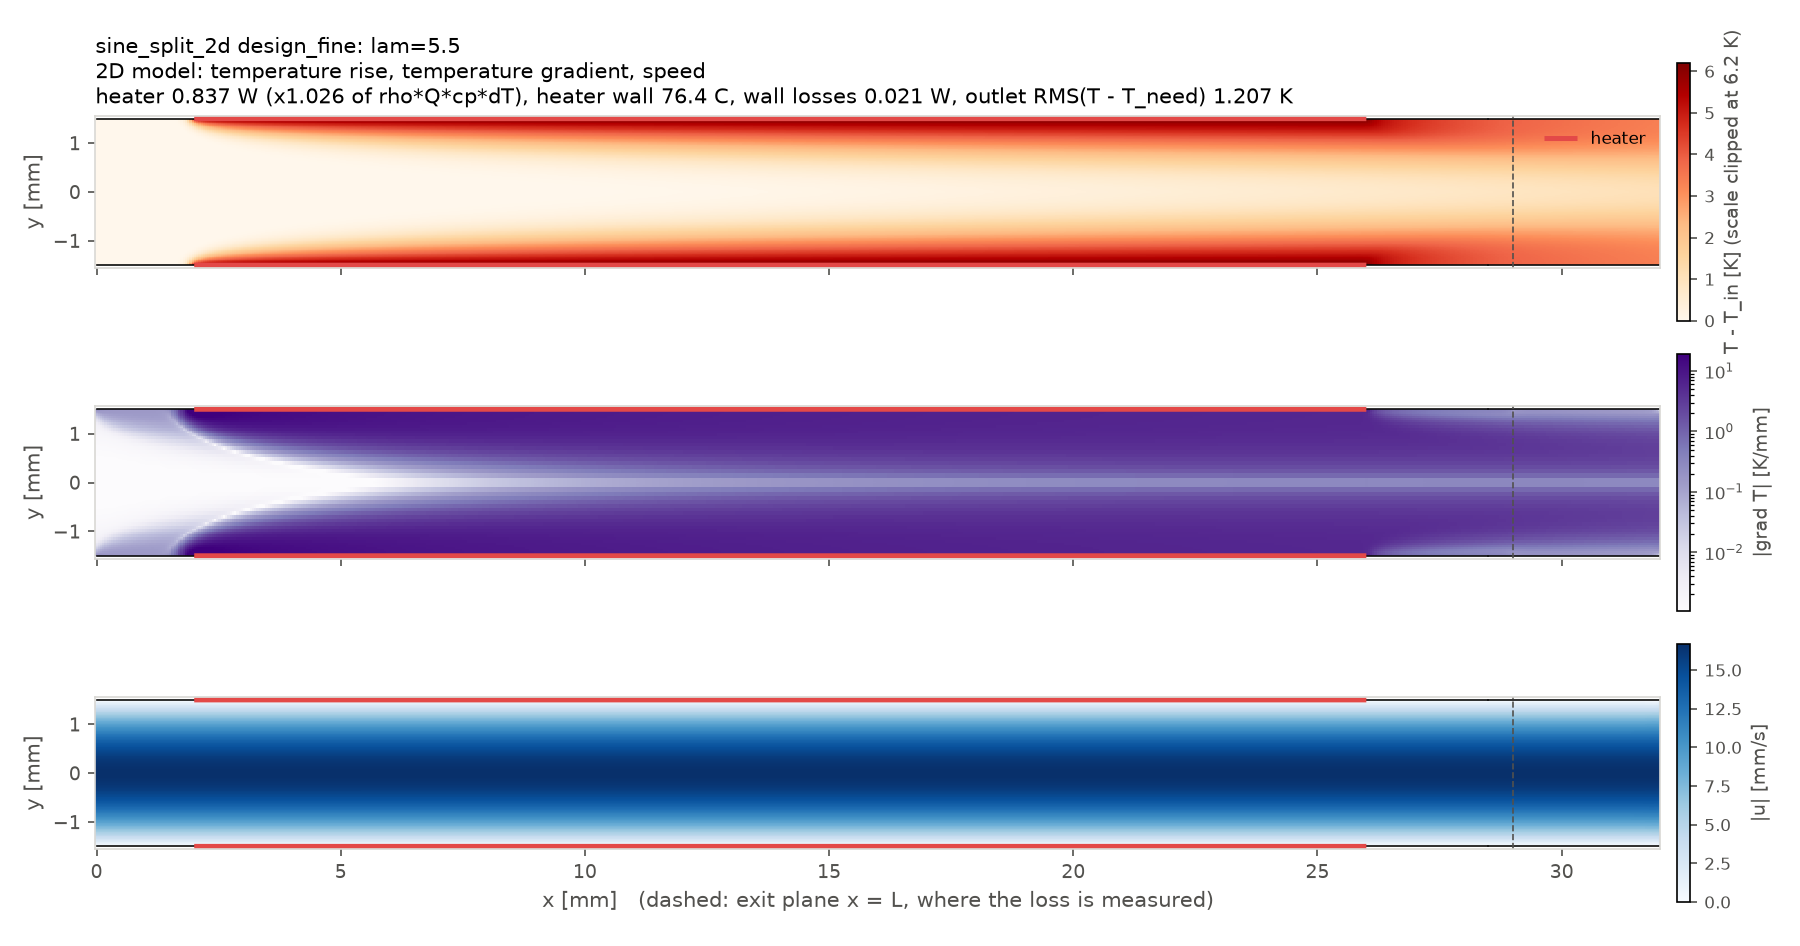
\includegraphics[width=0.95\textwidth,height=0.8\textheight,keepaspectratio]{runs/final_u2d_straight_ref_single_maps.png}
\caption{Temperature rise, temperature gradient and speed (mid-depth plane in 3D). Red: heated wall. The title's ``outlet RMS'' is the area-weighted $\ell_{2,\mathrm{area}}$.}
\end{figure}
\begin{figure}[H]\centering
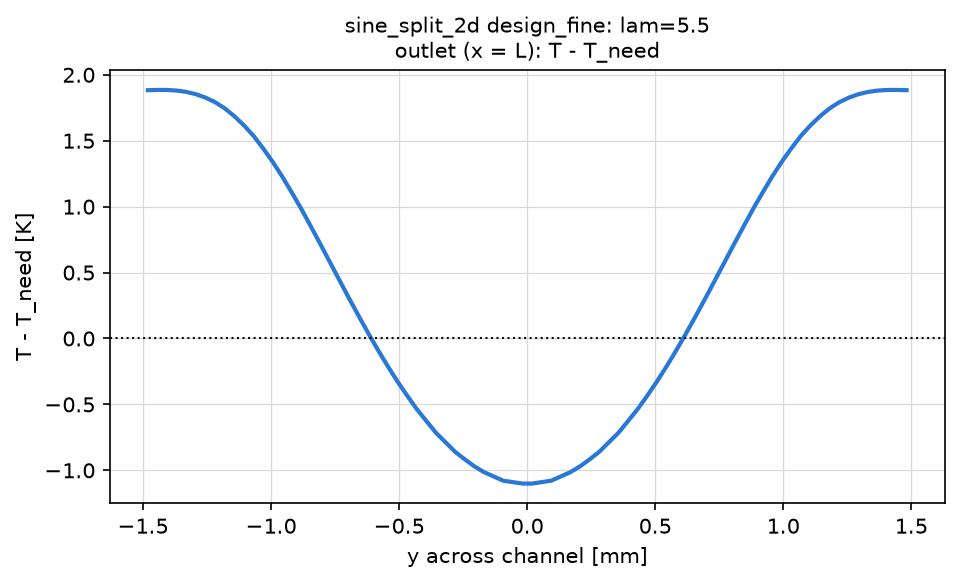
\includegraphics[width=0.75\textwidth,height=0.8\textheight,keepaspectratio]{runs/final_u2d_straight_ref_single_outlet.png}
\caption{Outlet temperature (and, in 3D, the outlet plane).}
\end{figure}
\begin{figure}[H]\centering
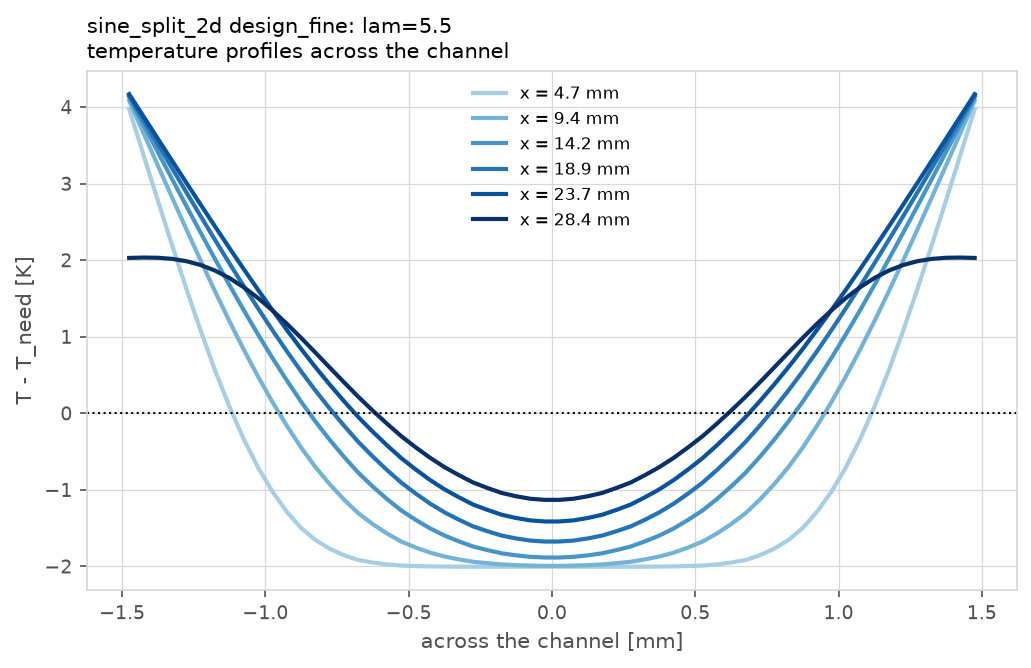
\includegraphics[width=0.62\textwidth,height=0.8\textheight,keepaspectratio]{runs/final_u2d_straight_ref_single_slices.png}
\caption{Temperature profiles across the channel at several $x$ stations.}
\end{figure}
\begin{figure}[H]\centering
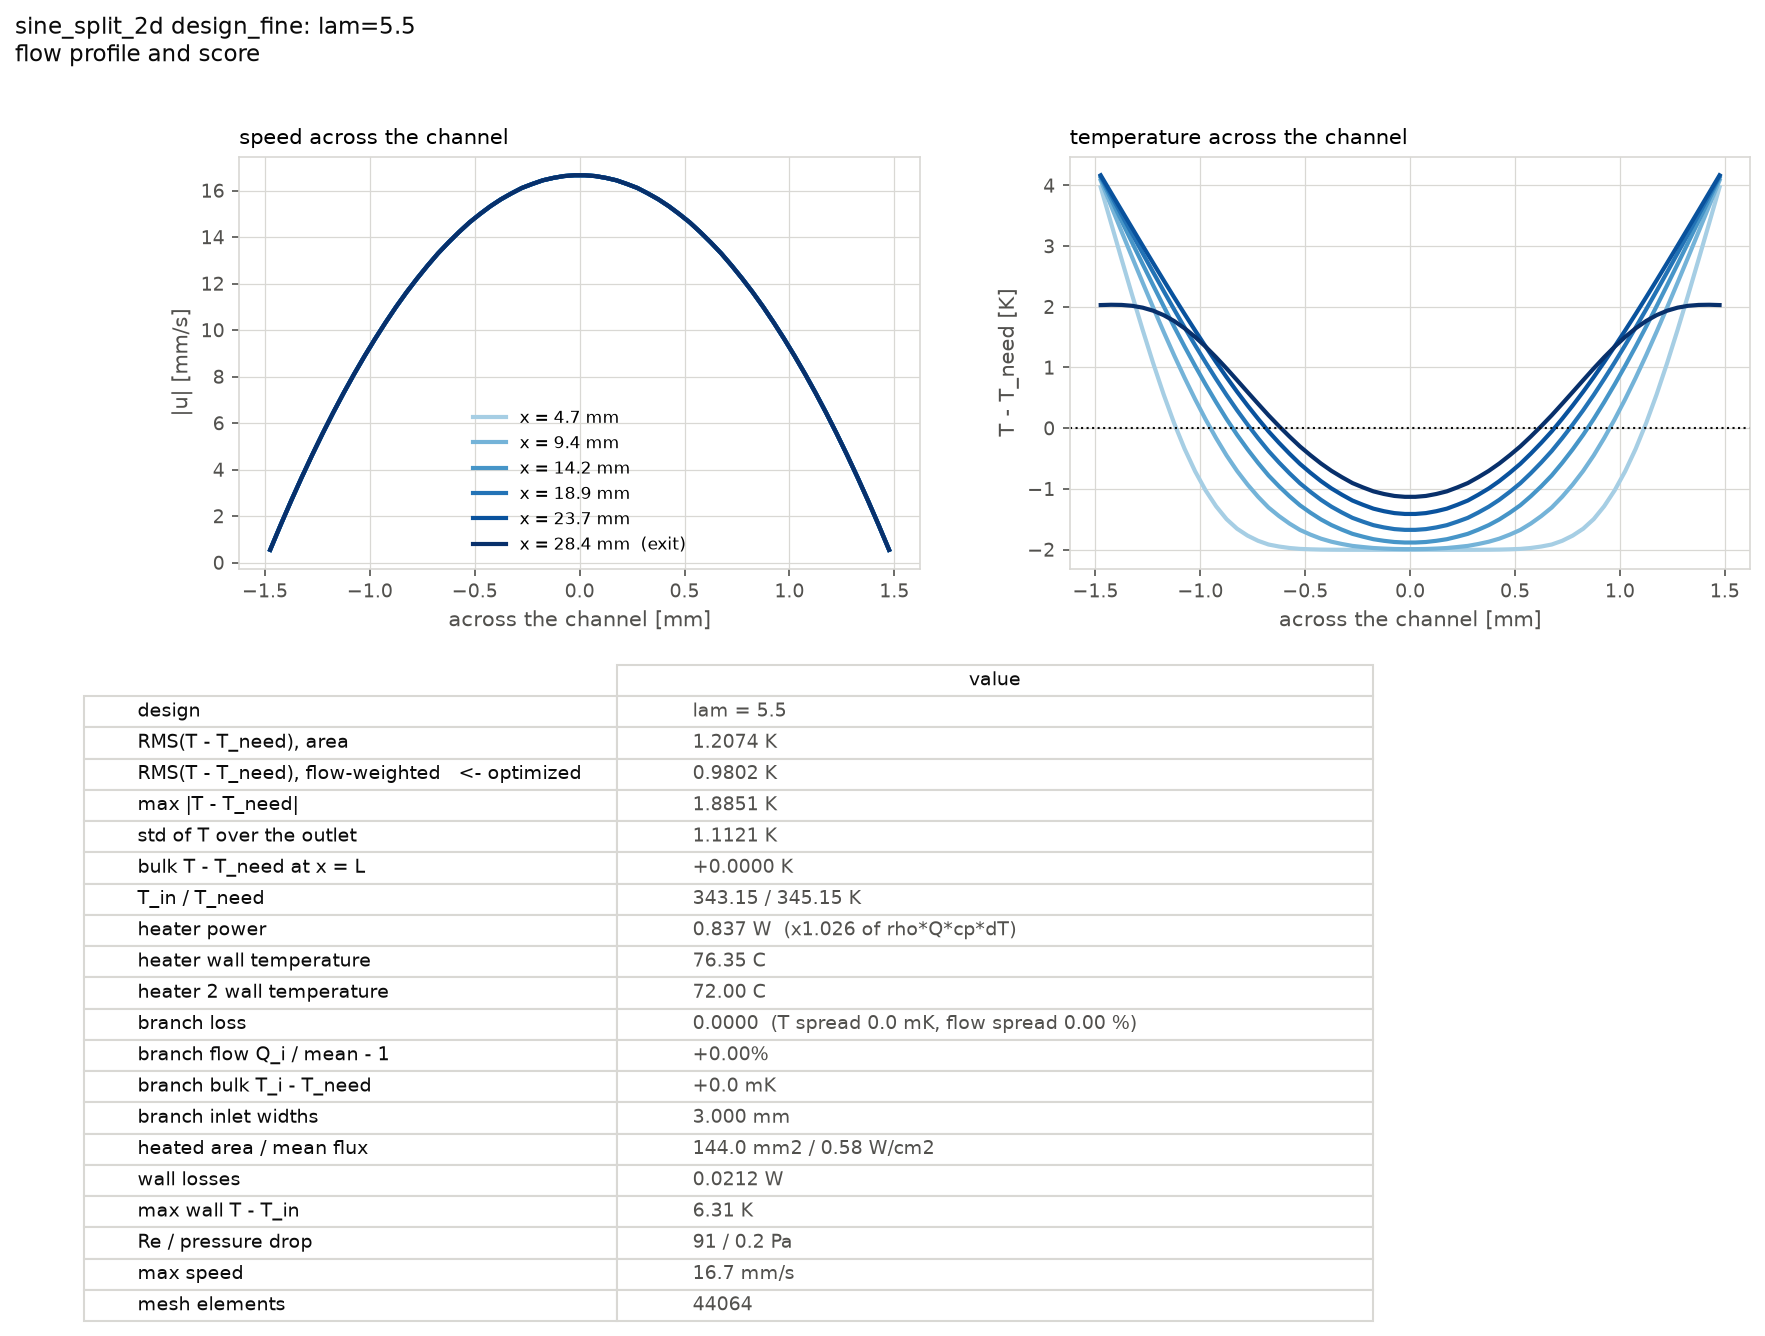
\includegraphics[width=0.8\textwidth,height=0.8\textheight,keepaspectratio]{runs/final_u2d_straight_ref_single_profile.png}
\caption{Speed and temperature across the channel at several $x$ stations, and the full score table of the design.}
\end{figure}
\begin{figure}[H]\centering
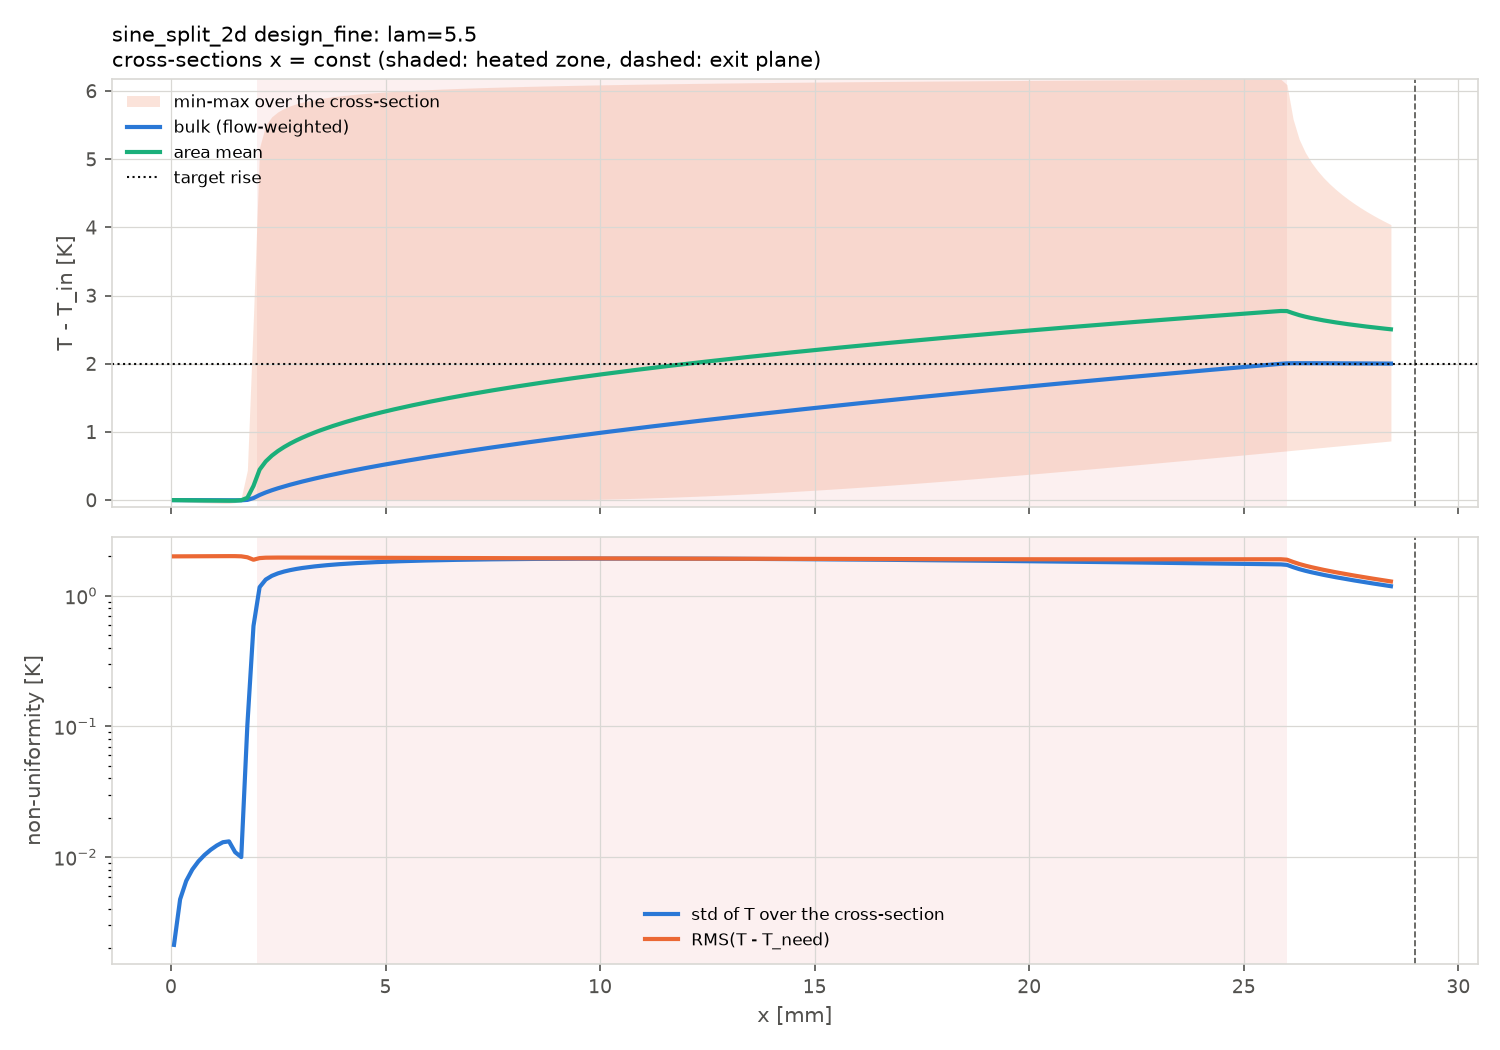
\includegraphics[width=0.8\textwidth,height=0.8\textheight,keepaspectratio]{runs/final_u2d_straight_ref_single_along_x.png}
\caption{Bulk, mean, min and max temperature along the channel.}
\end{figure}
\clearpage
\subsubsection*{2D straight reference, best heater window (start 0, length 10\,\%): 388\mK}
\noindent\texttt{runs/final\_u2d\_straight\_ref}\par\medskip
\begin{figure}[H]\centering
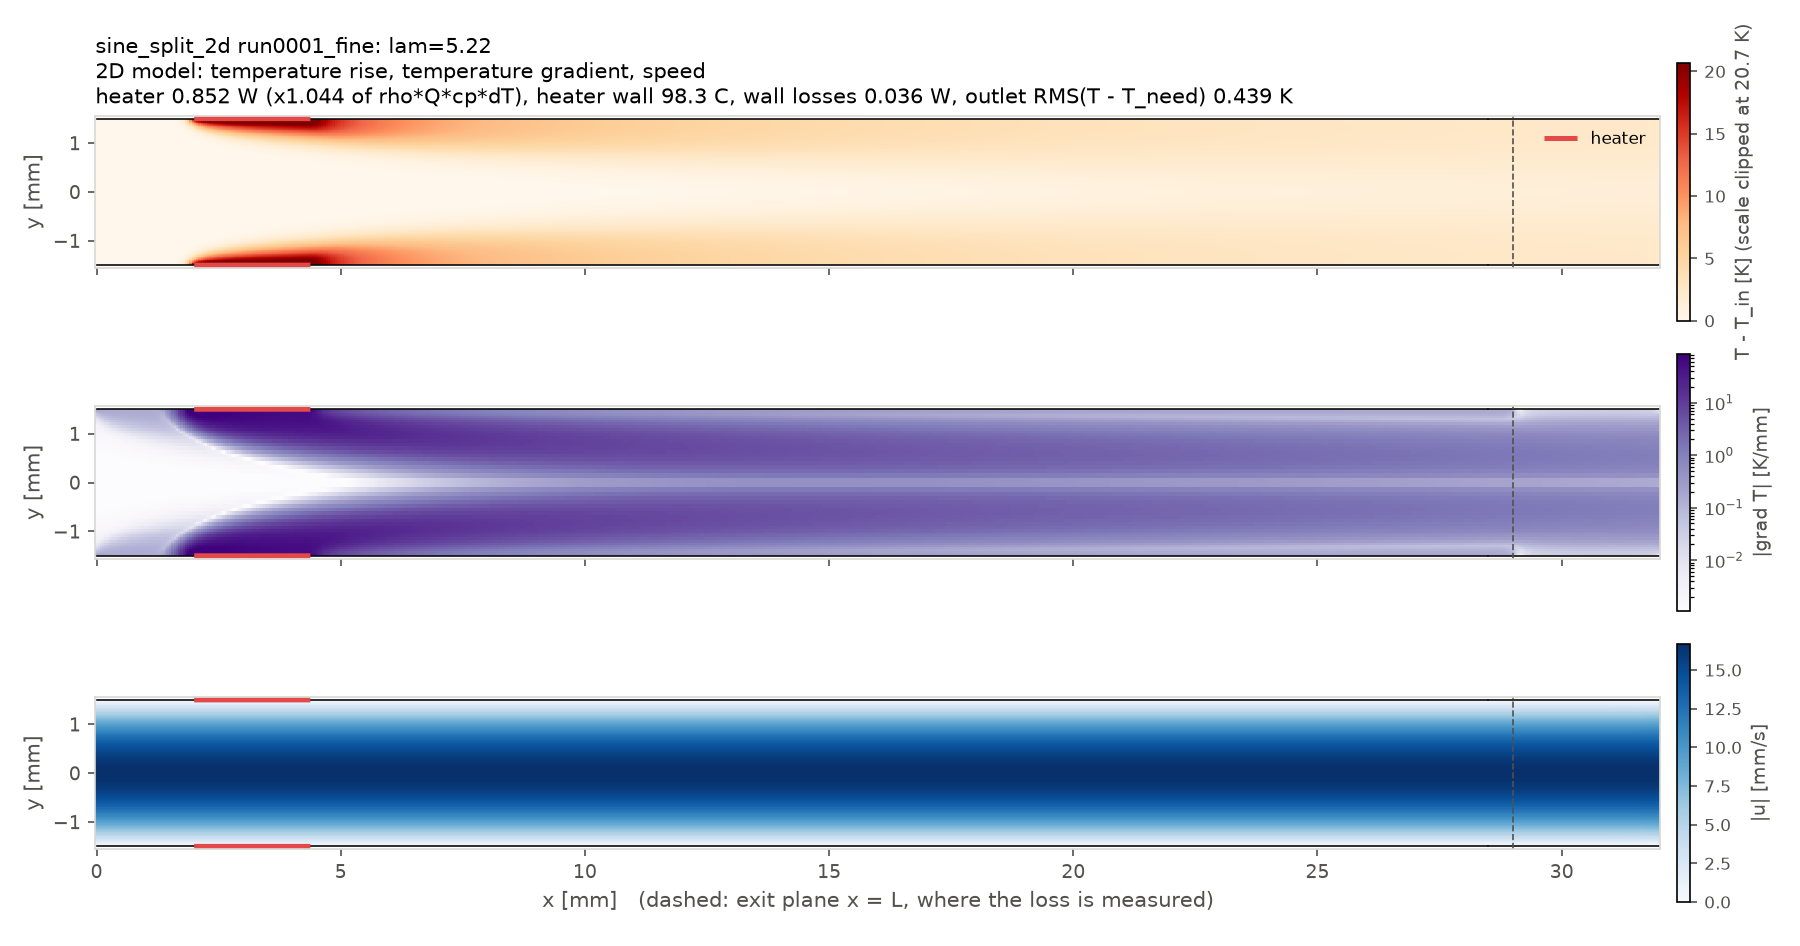
\includegraphics[width=0.95\textwidth,height=0.8\textheight,keepaspectratio]{runs/final_u2d_straight_ref_maps.png}
\caption{Temperature rise, temperature gradient and speed (mid-depth plane in 3D). Red: heated wall. The title's ``outlet RMS'' is the area-weighted $\ell_{2,\mathrm{area}}$.}
\end{figure}
\begin{figure}[H]\centering
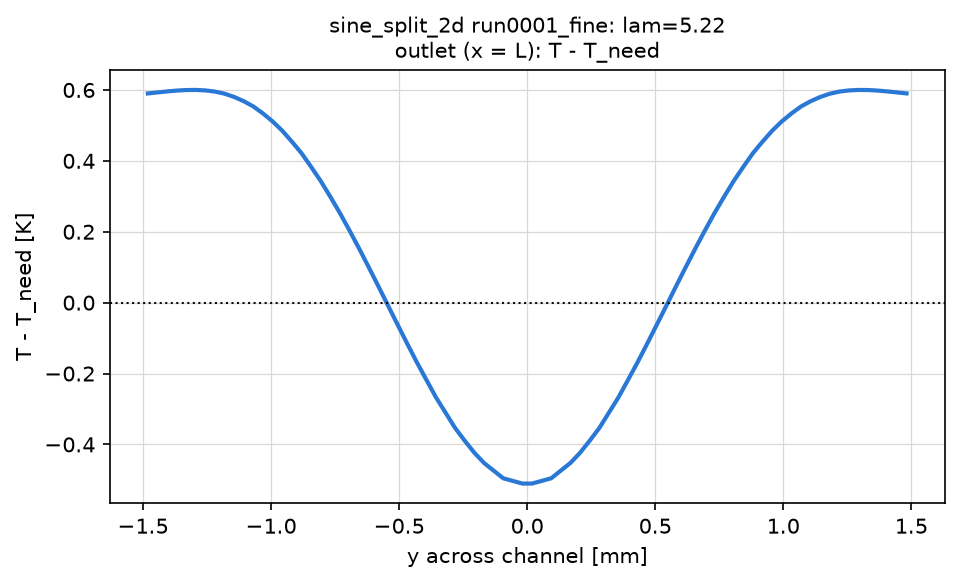
\includegraphics[width=0.75\textwidth,height=0.8\textheight,keepaspectratio]{runs/final_u2d_straight_ref_outlet.png}
\caption{Outlet temperature (and, in 3D, the outlet plane).}
\end{figure}
\begin{figure}[H]\centering
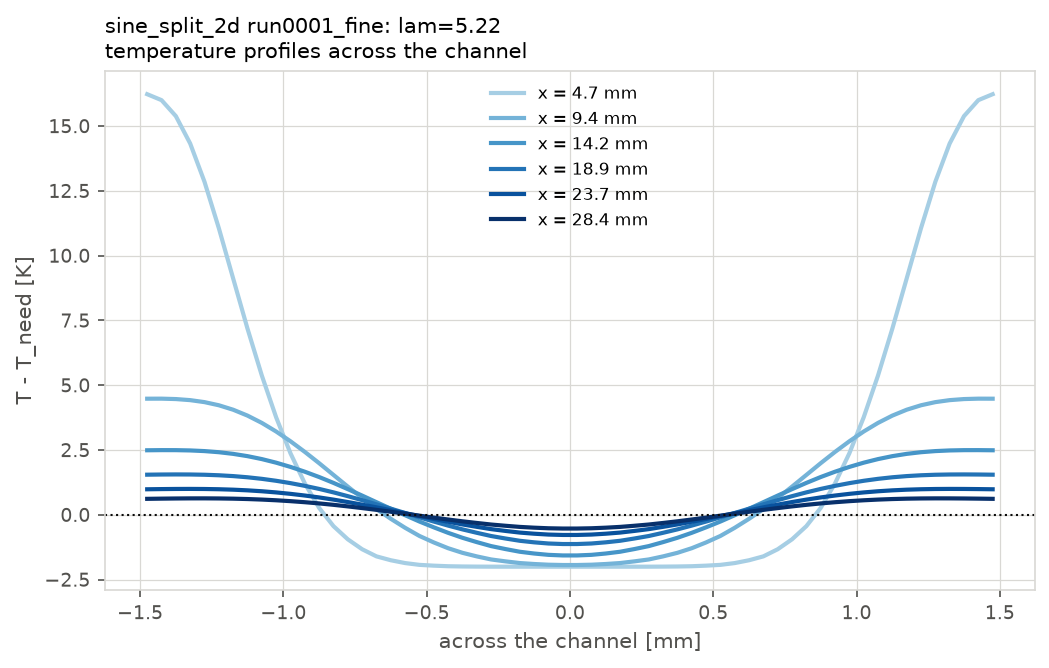
\includegraphics[width=0.62\textwidth,height=0.8\textheight,keepaspectratio]{runs/final_u2d_straight_ref_slices.png}
\caption{Temperature profiles across the channel at several $x$ stations.}
\end{figure}
\begin{figure}[H]\centering
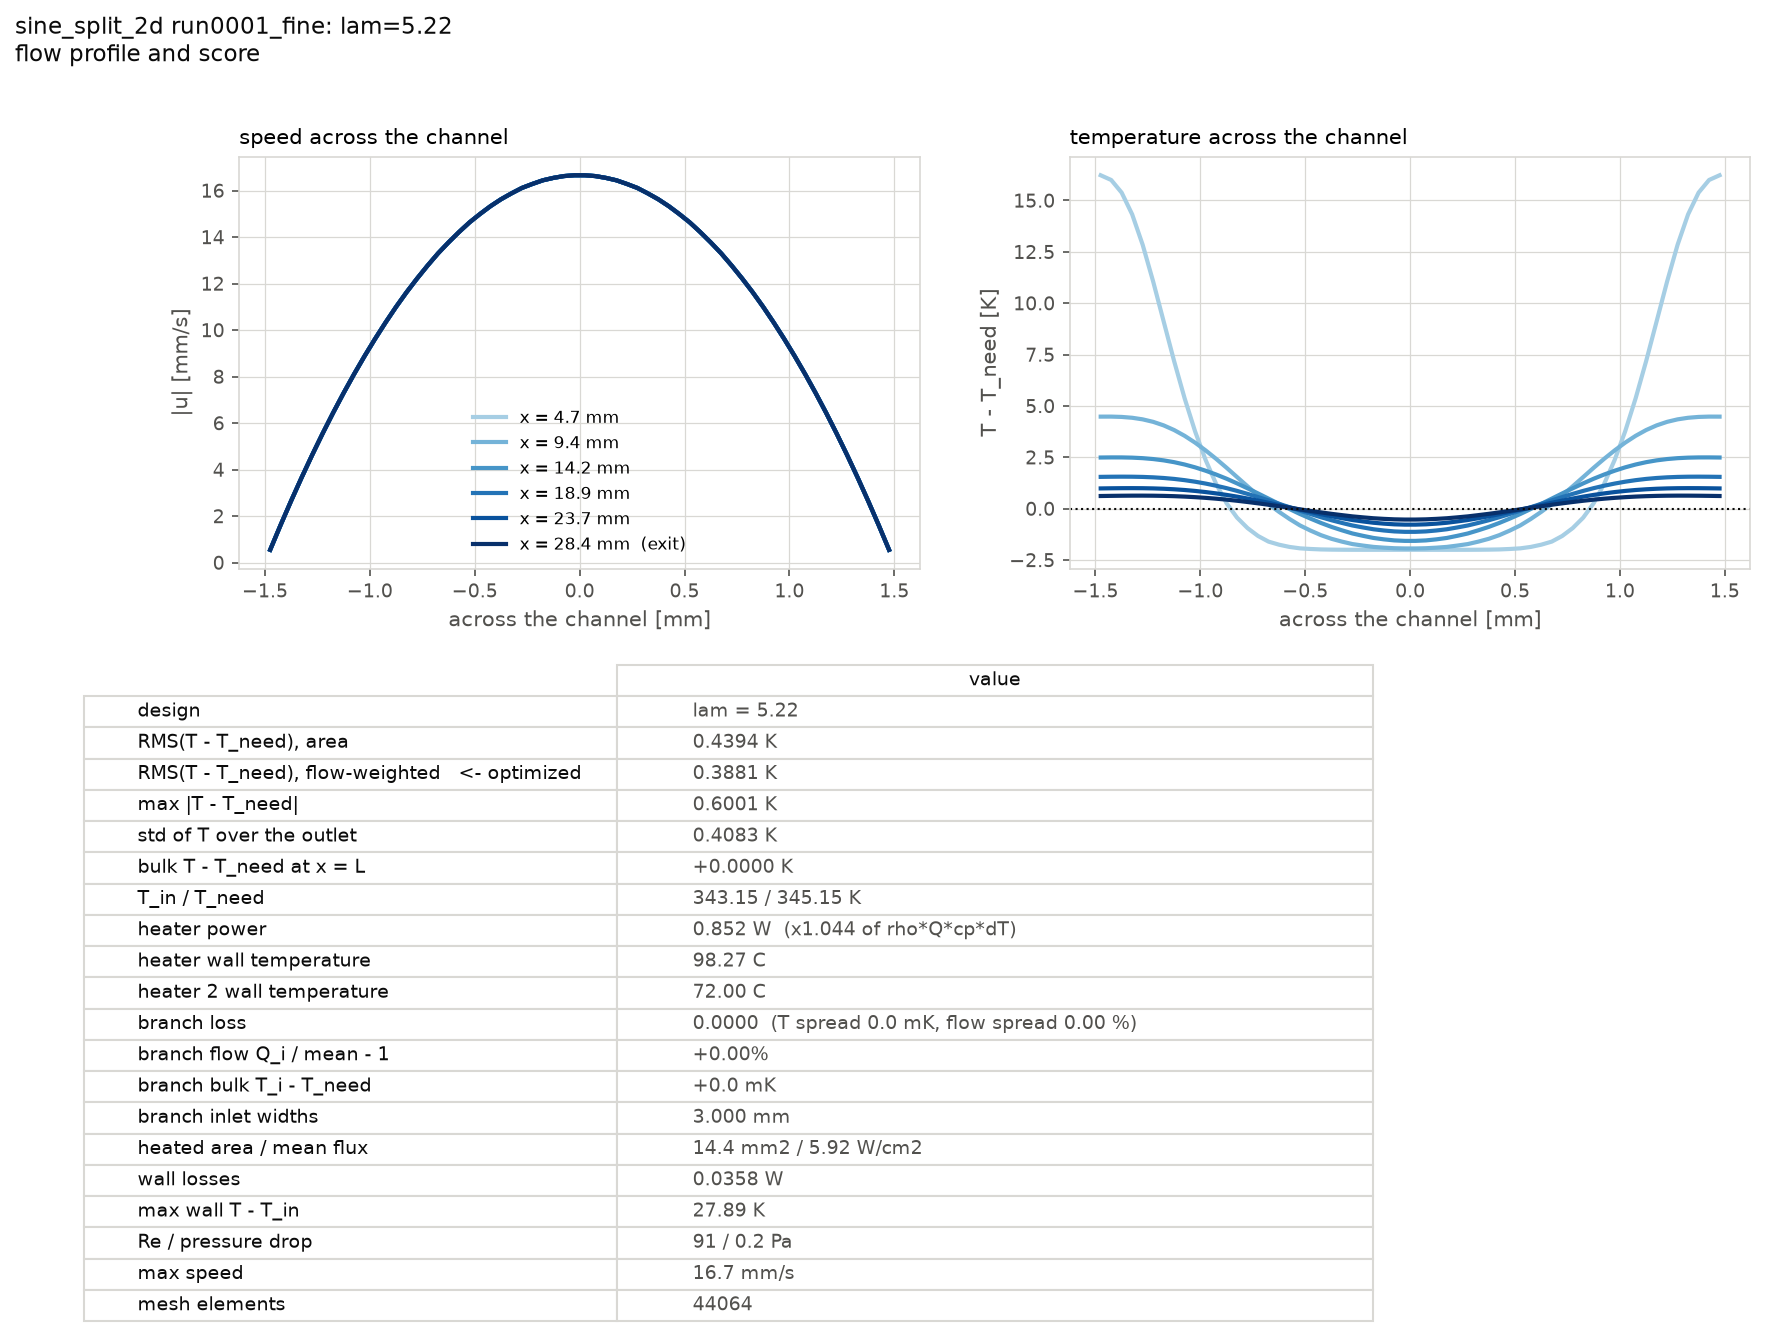
\includegraphics[width=0.8\textwidth,height=0.8\textheight,keepaspectratio]{runs/final_u2d_straight_ref_profile.png}
\caption{Speed and temperature across the channel at several $x$ stations, and the full score table of the design.}
\end{figure}
\begin{figure}[H]\centering
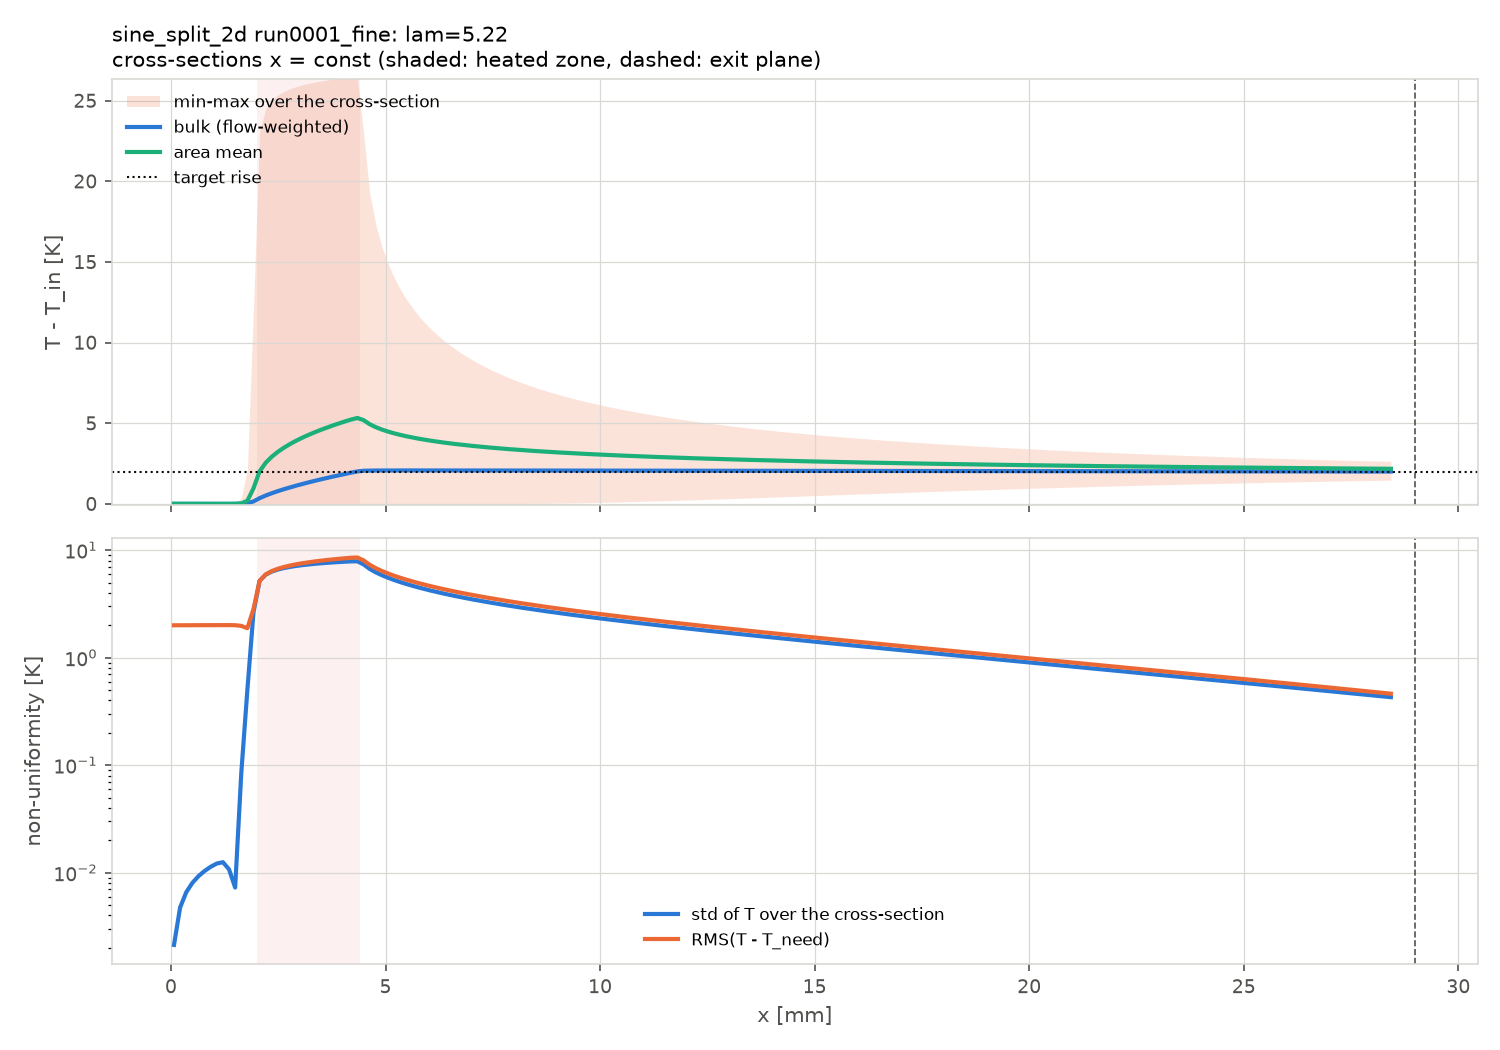
\includegraphics[width=0.8\textwidth,height=0.8\textheight,keepaspectratio]{runs/final_u2d_straight_ref_along_x.png}
\caption{Bulk, mean, min and max temperature along the channel.}
\end{figure}
\clearpage
\subsubsection*{2D sine, BO best \#50 ($\lambda$ 11.14, $a$ 1, heater 30\,\%): 120\mK}
\noindent\texttt{runs/final\_u2d\_sine}\par\medskip
\begin{figure}[H]\centering
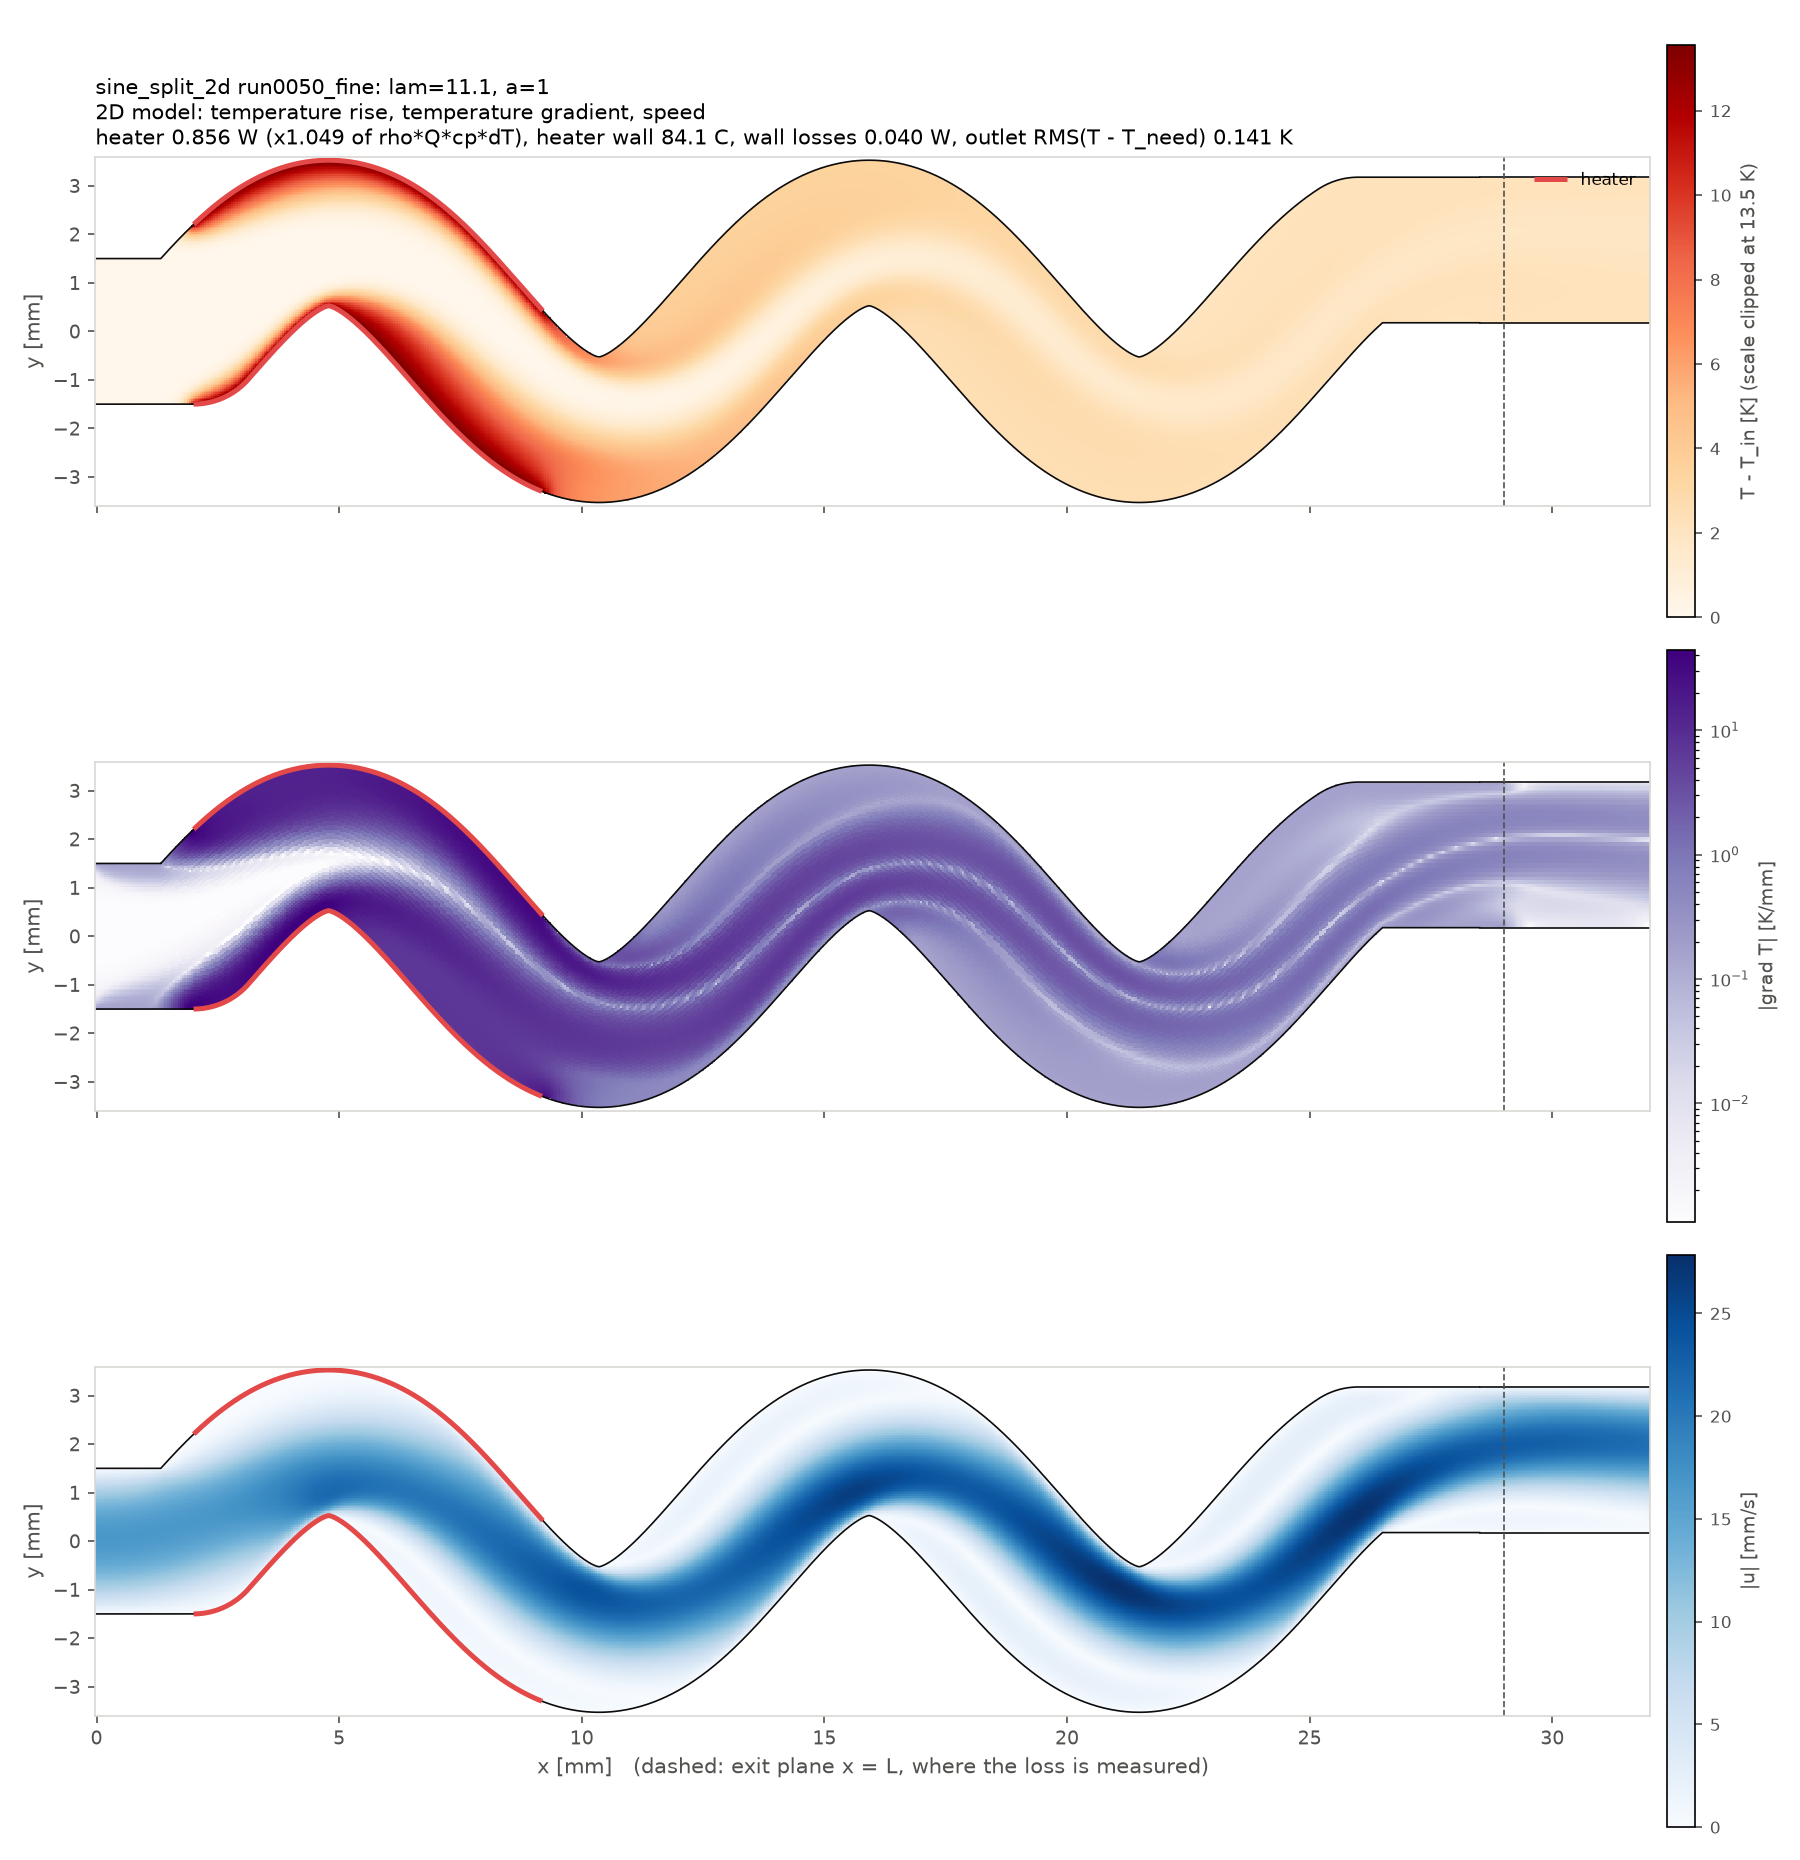
\includegraphics[width=0.95\textwidth,height=0.8\textheight,keepaspectratio]{runs/final_u2d_sine_maps.png}
\caption{Temperature rise, temperature gradient and speed (mid-depth plane in 3D). Red: heated wall. The title's ``outlet RMS'' is the area-weighted $\ell_{2,\mathrm{area}}$.}
\end{figure}
\begin{figure}[H]\centering
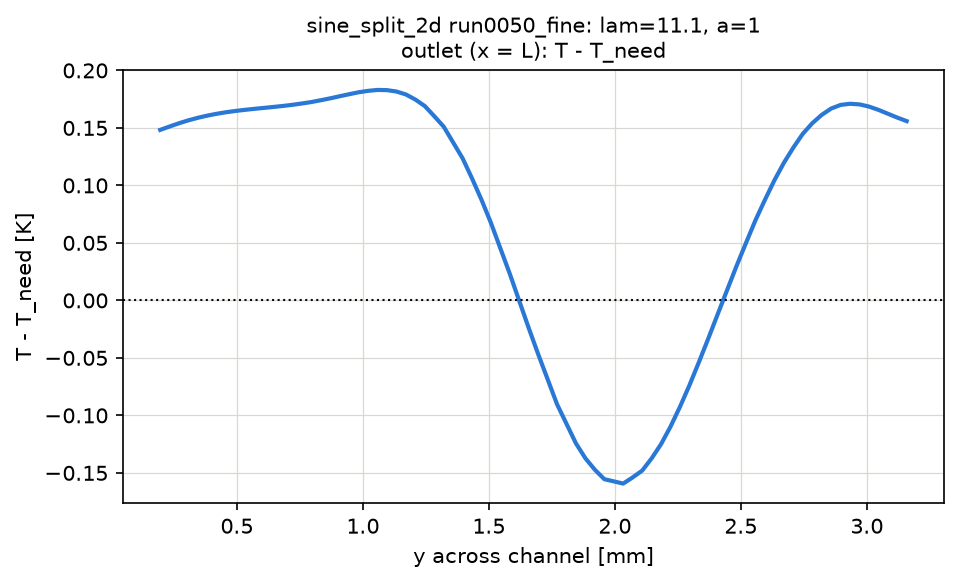
\includegraphics[width=0.75\textwidth,height=0.8\textheight,keepaspectratio]{runs/final_u2d_sine_outlet.png}
\caption{Outlet temperature (and, in 3D, the outlet plane).}
\end{figure}
\begin{figure}[H]\centering
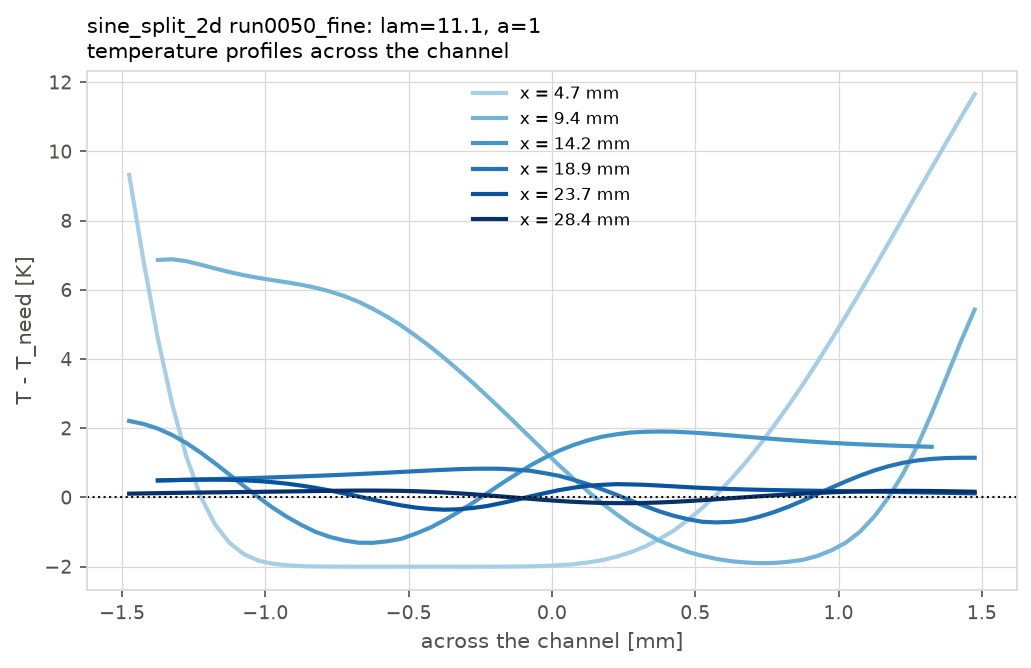
\includegraphics[width=0.62\textwidth,height=0.8\textheight,keepaspectratio]{runs/final_u2d_sine_slices.png}
\caption{Temperature profiles across the channel at several $x$ stations.}
\end{figure}
\begin{figure}[H]\centering
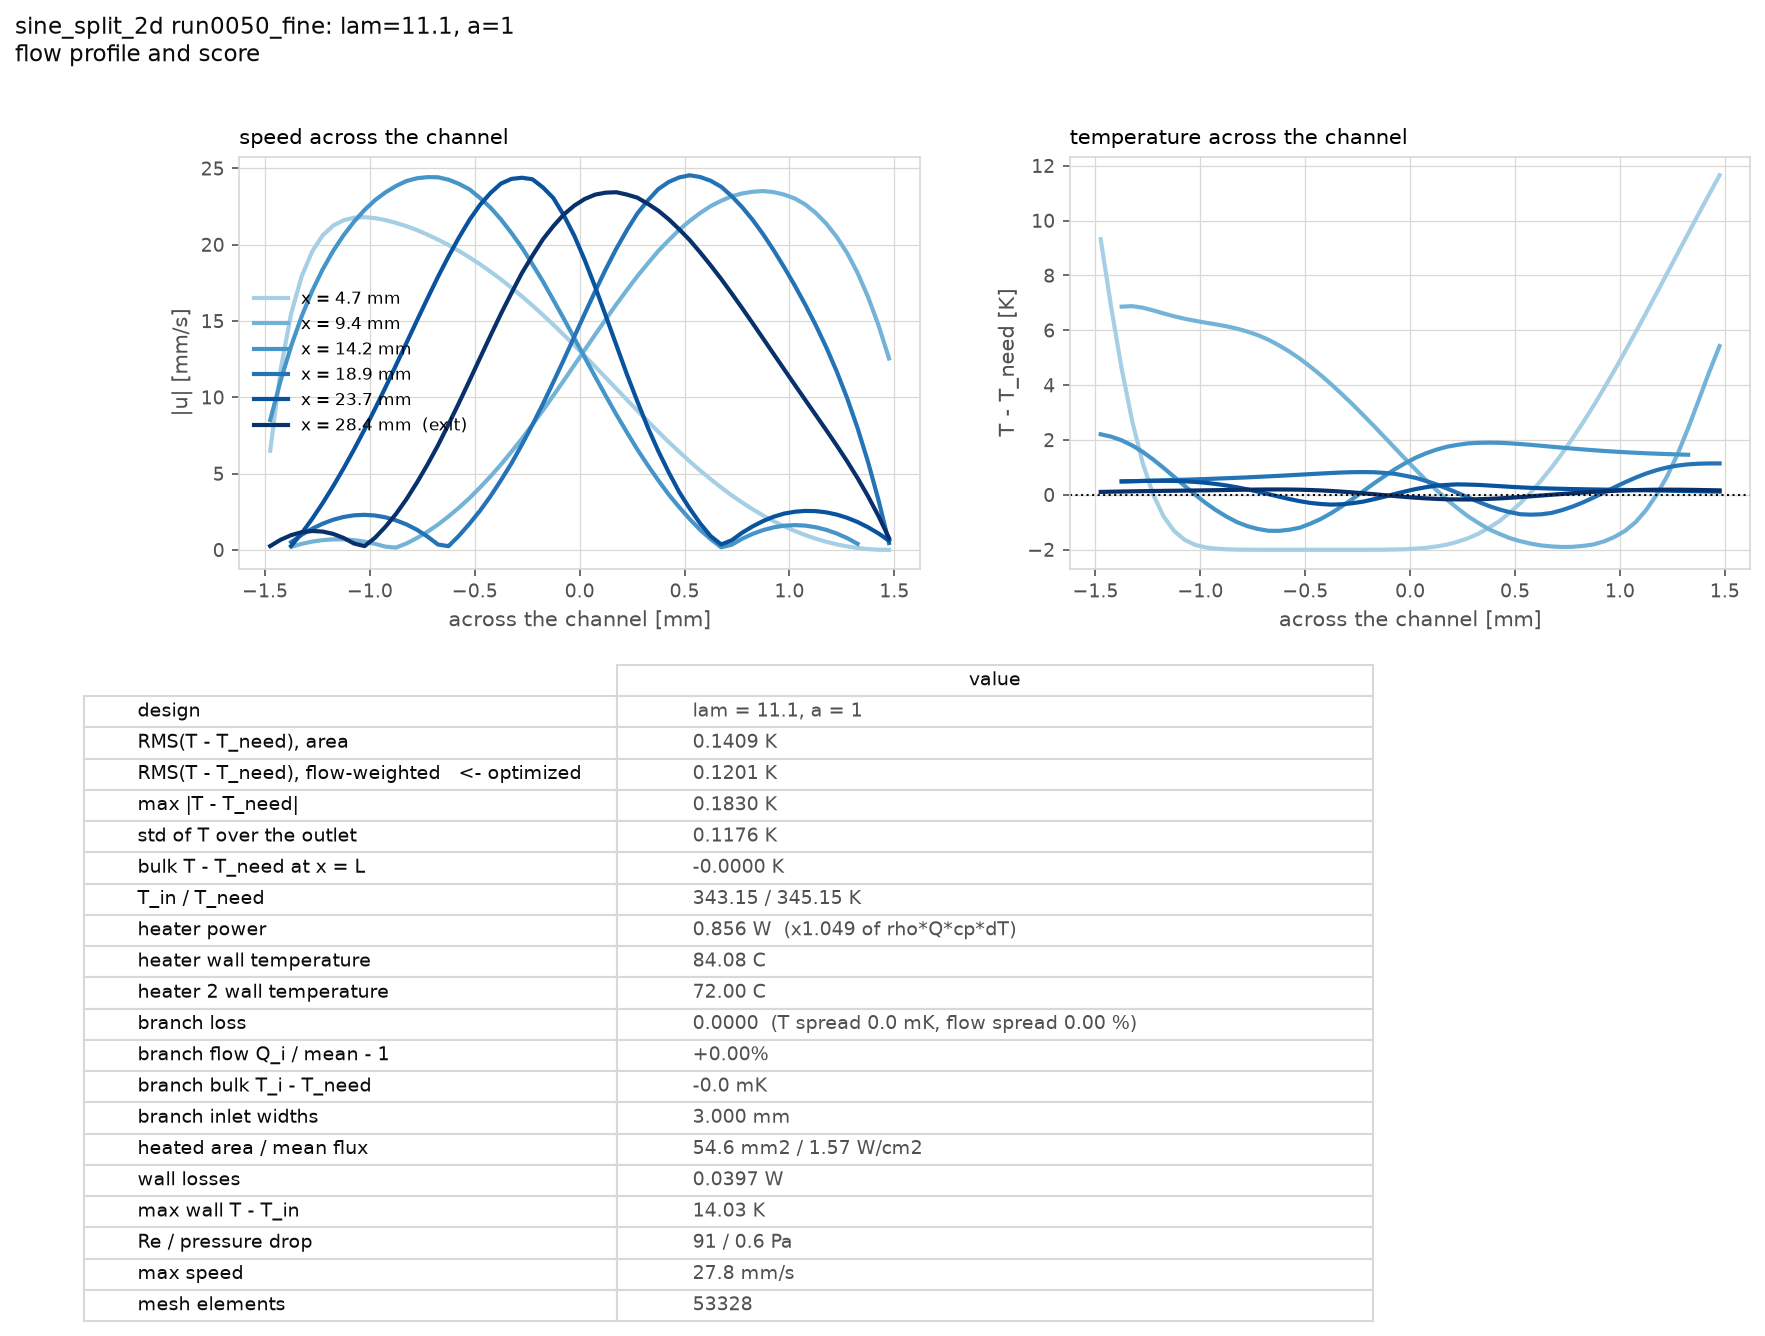
\includegraphics[width=0.8\textwidth,height=0.8\textheight,keepaspectratio]{runs/final_u2d_sine_profile.png}
\caption{Speed and temperature across the channel at several $x$ stations, and the full score table of the design.}
\end{figure}
\begin{figure}[H]\centering
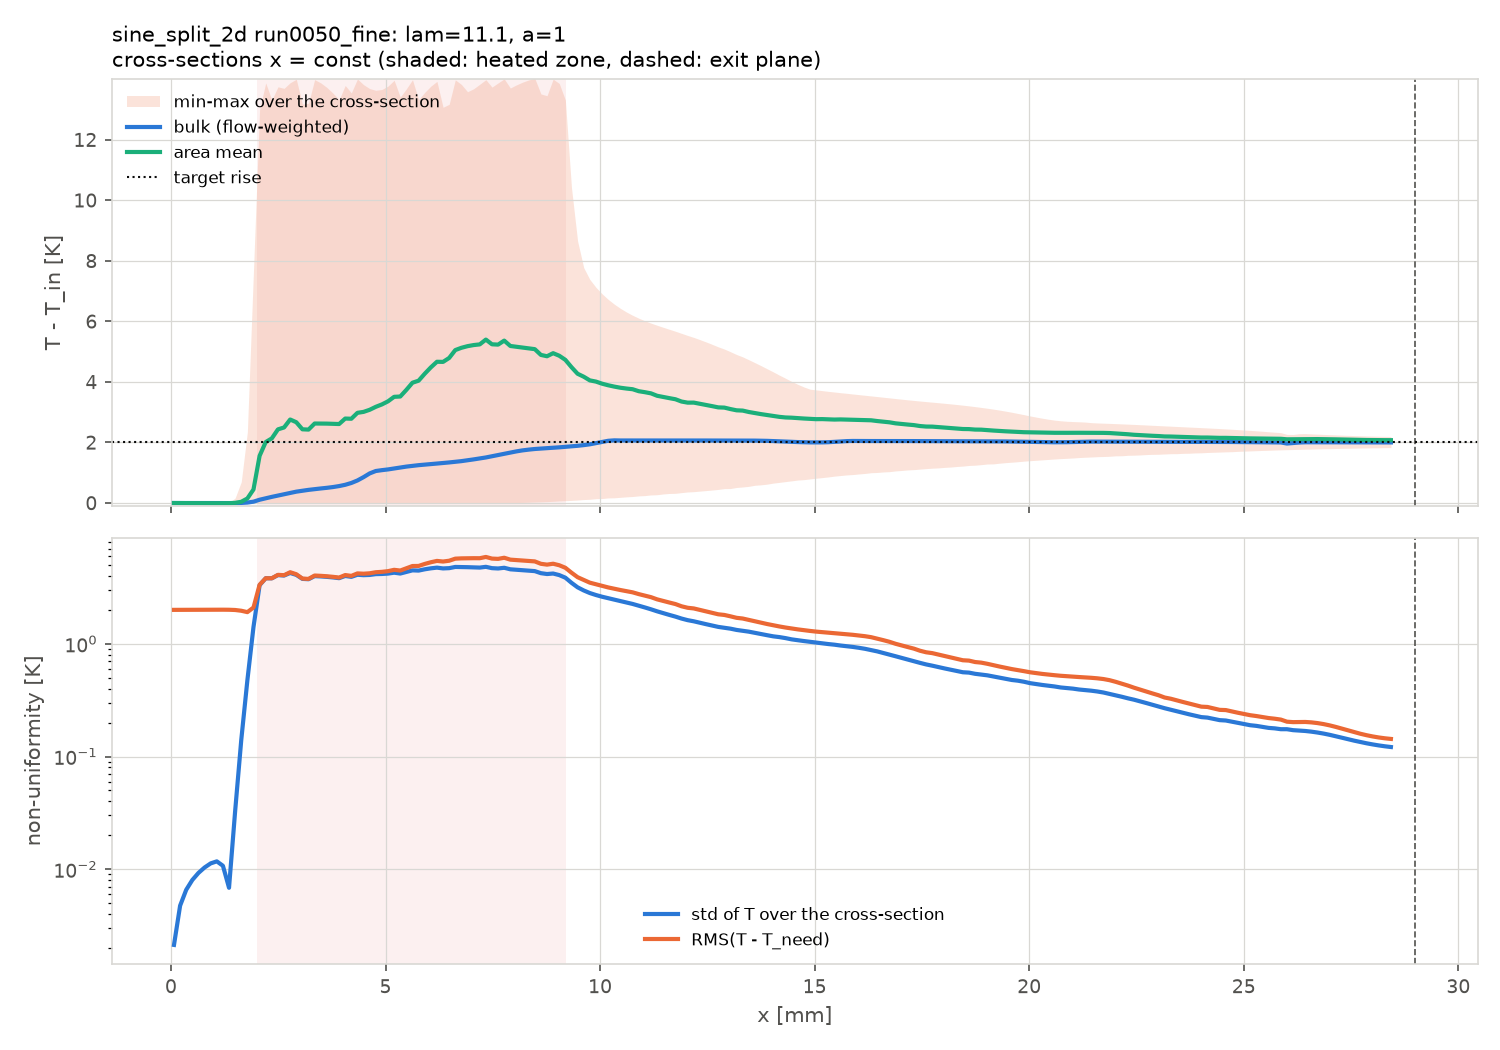
\includegraphics[width=0.8\textwidth,height=0.8\textheight,keepaspectratio]{runs/final_u2d_sine_along_x.png}
\caption{Bulk, mean, min and max temperature along the channel.}
\end{figure}
\begin{figure}[H]\centering
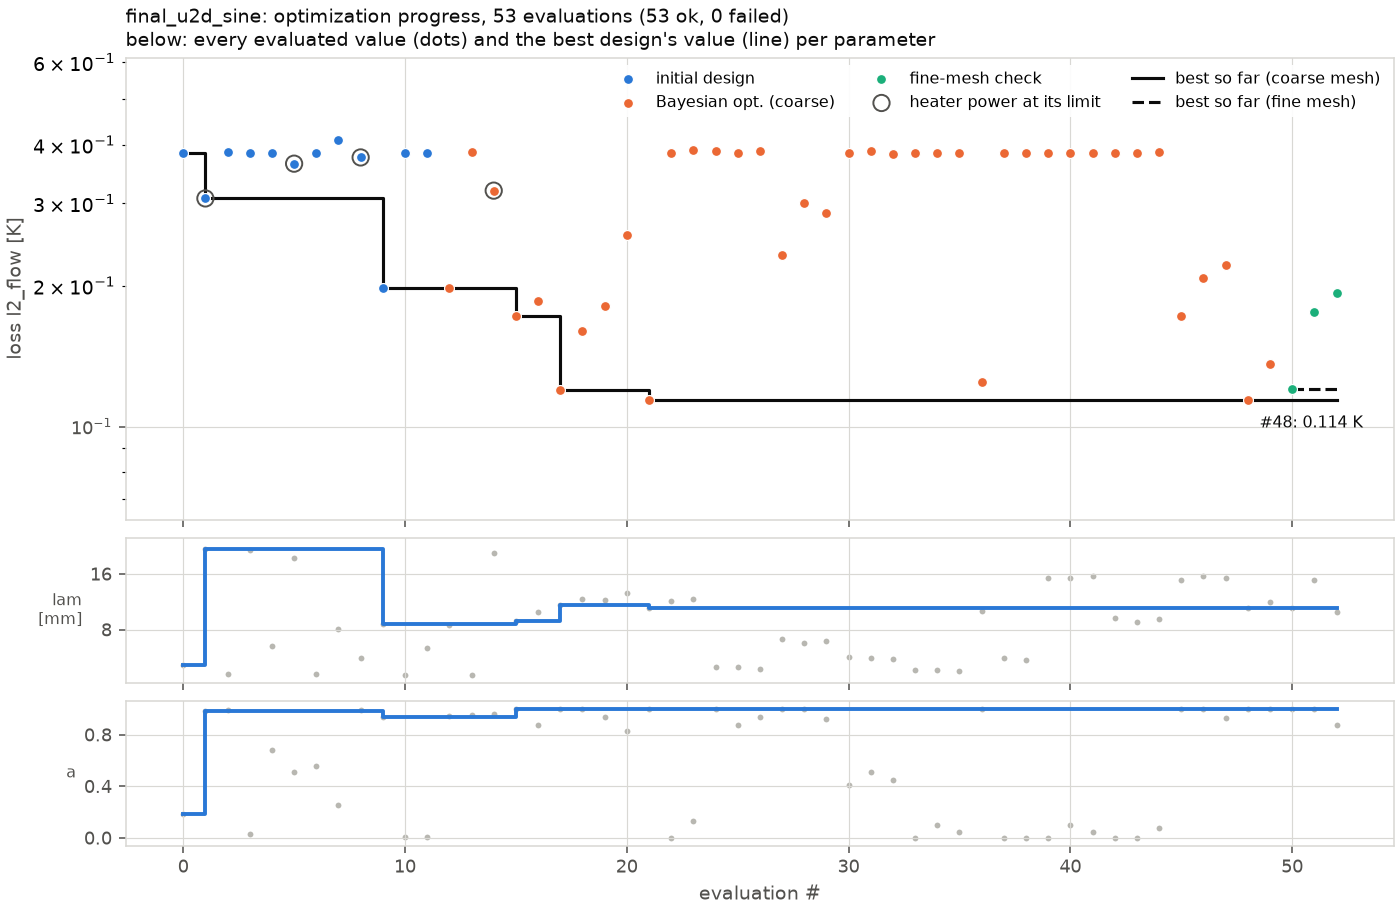
\includegraphics[width=0.85\textwidth]{runs/final_u2d_sine_progress_loss.png}
\caption{Search history: loss of every evaluation, best so far, and the parameters.}
\end{figure}
\clearpage
\subsubsection*{2D sine, grid best \#112 ($\lambda$ 11.10, $a$ 1, heater 30\,\%): 120\mK}
\noindent\texttt{runs/final\_u2d\_sine\_grid}\par\medskip
\begin{figure}[H]\centering
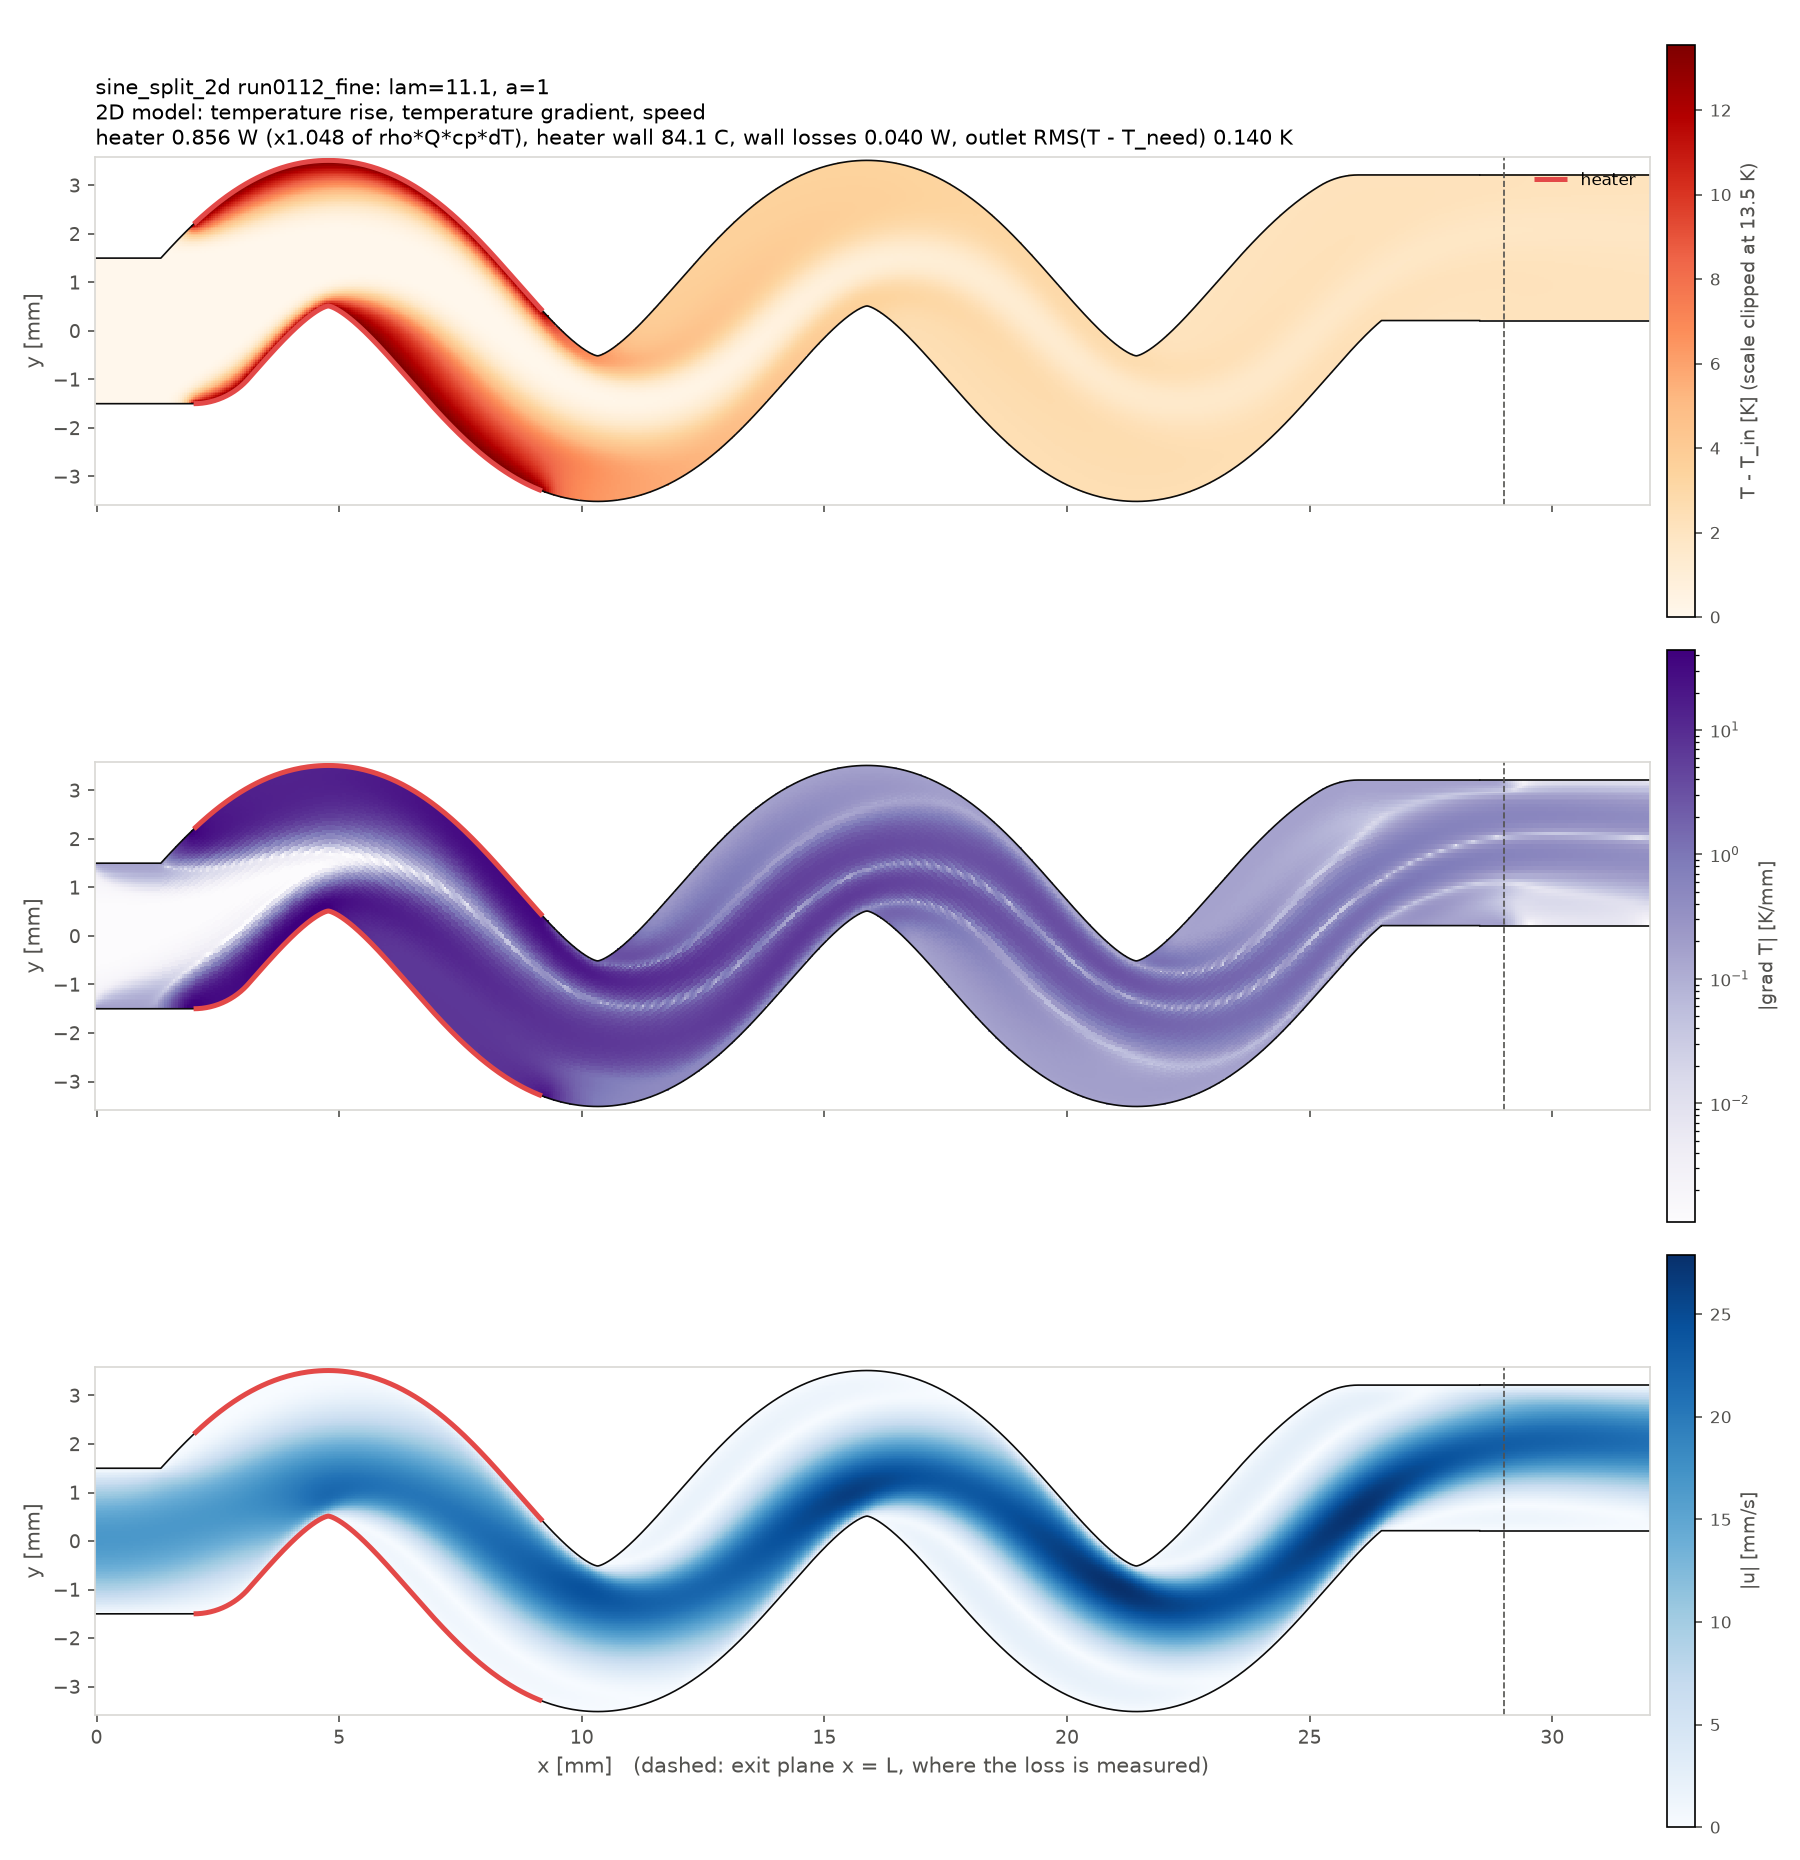
\includegraphics[width=0.95\textwidth,height=0.8\textheight,keepaspectratio]{runs/final_u2d_sine_grid_maps.png}
\caption{Temperature rise, temperature gradient and speed (mid-depth plane in 3D). Red: heated wall. The title's ``outlet RMS'' is the area-weighted $\ell_{2,\mathrm{area}}$.}
\end{figure}
\begin{figure}[H]\centering
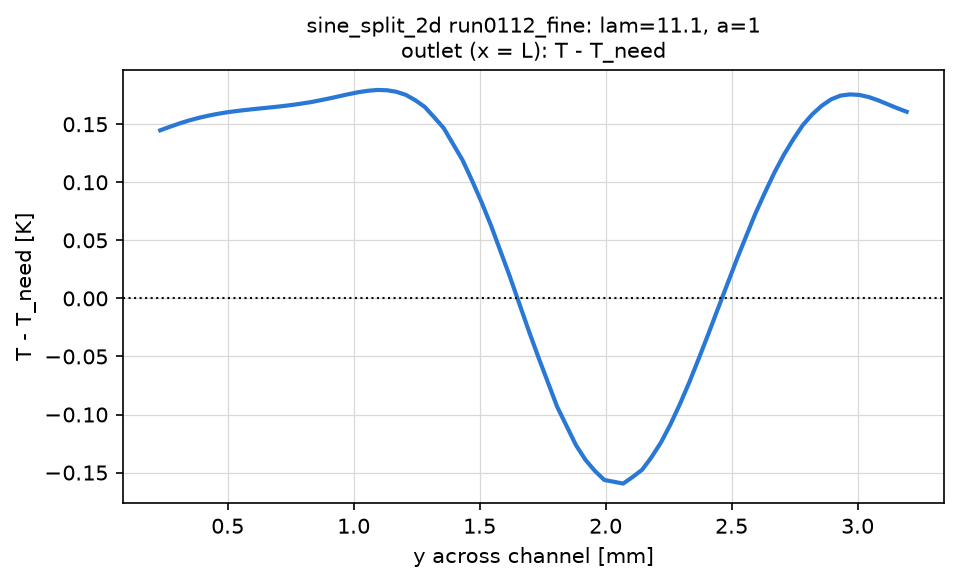
\includegraphics[width=0.75\textwidth,height=0.8\textheight,keepaspectratio]{runs/final_u2d_sine_grid_outlet.png}
\caption{Outlet temperature (and, in 3D, the outlet plane).}
\end{figure}
\begin{figure}[H]\centering
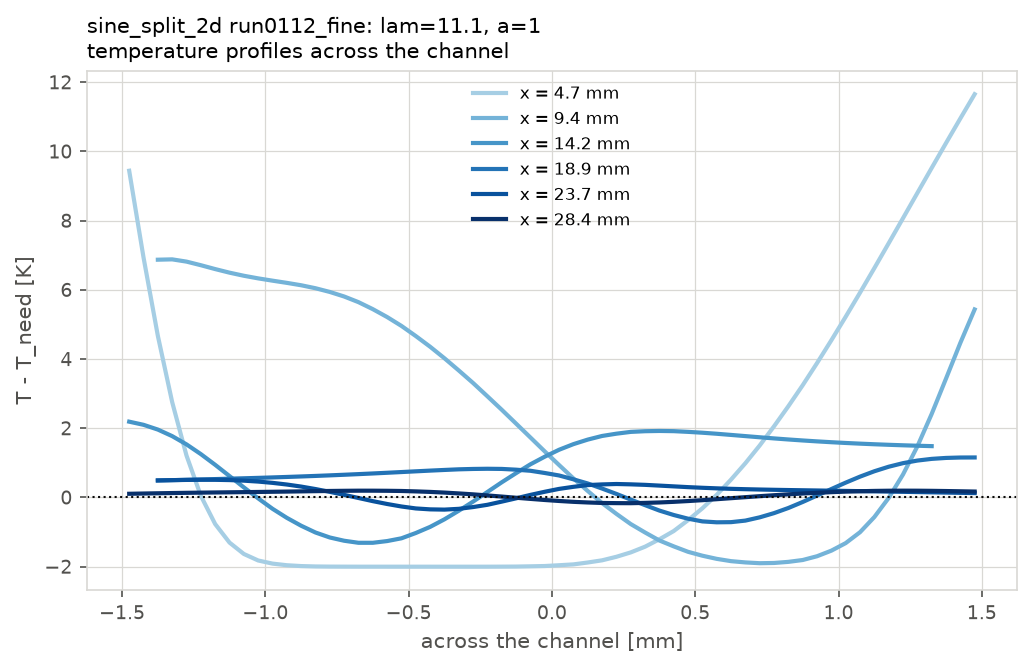
\includegraphics[width=0.62\textwidth,height=0.8\textheight,keepaspectratio]{runs/final_u2d_sine_grid_slices.png}
\caption{Temperature profiles across the channel at several $x$ stations.}
\end{figure}
\begin{figure}[H]\centering
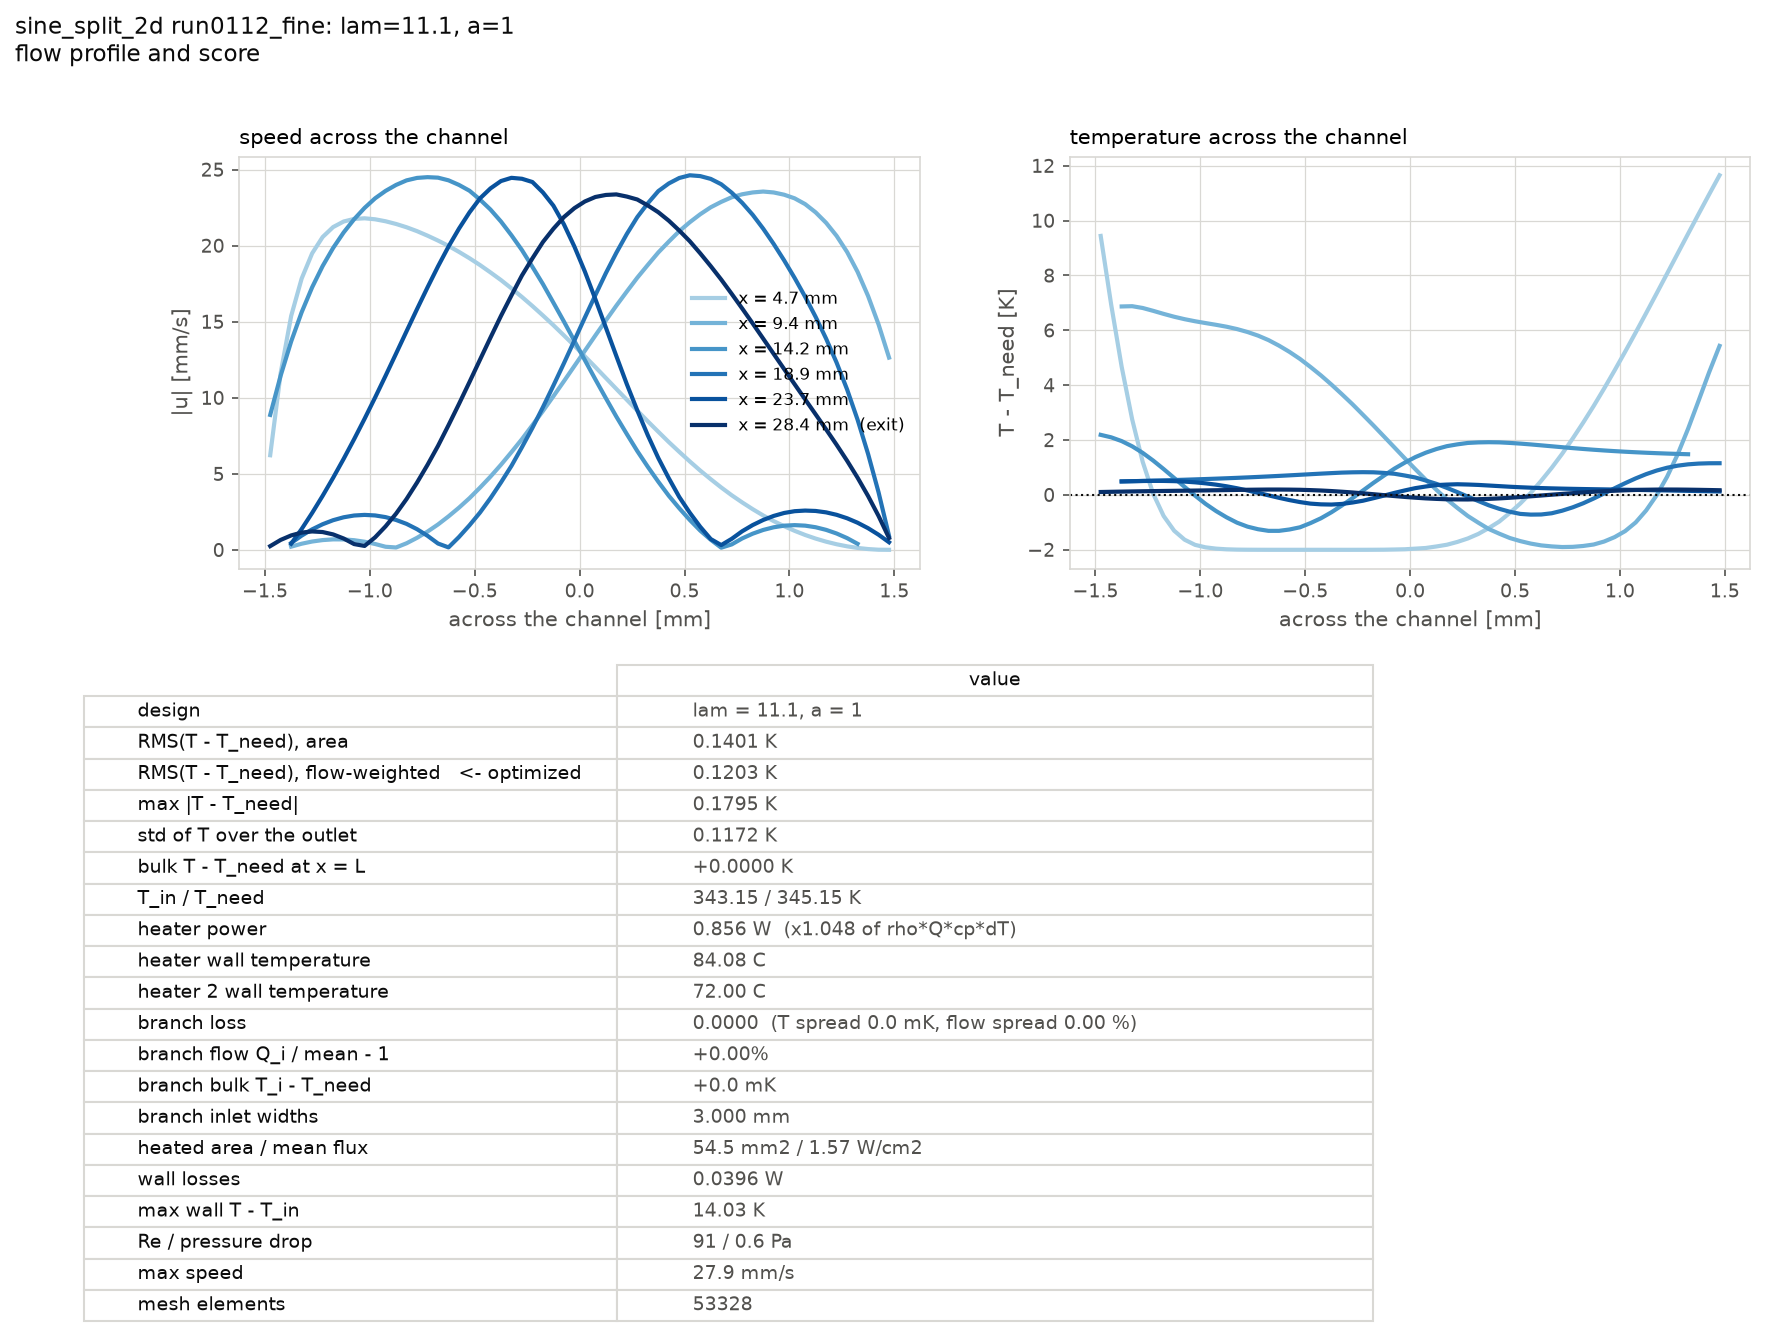
\includegraphics[width=0.8\textwidth,height=0.8\textheight,keepaspectratio]{runs/final_u2d_sine_grid_profile.png}
\caption{Speed and temperature across the channel at several $x$ stations, and the full score table of the design.}
\end{figure}
\begin{figure}[H]\centering
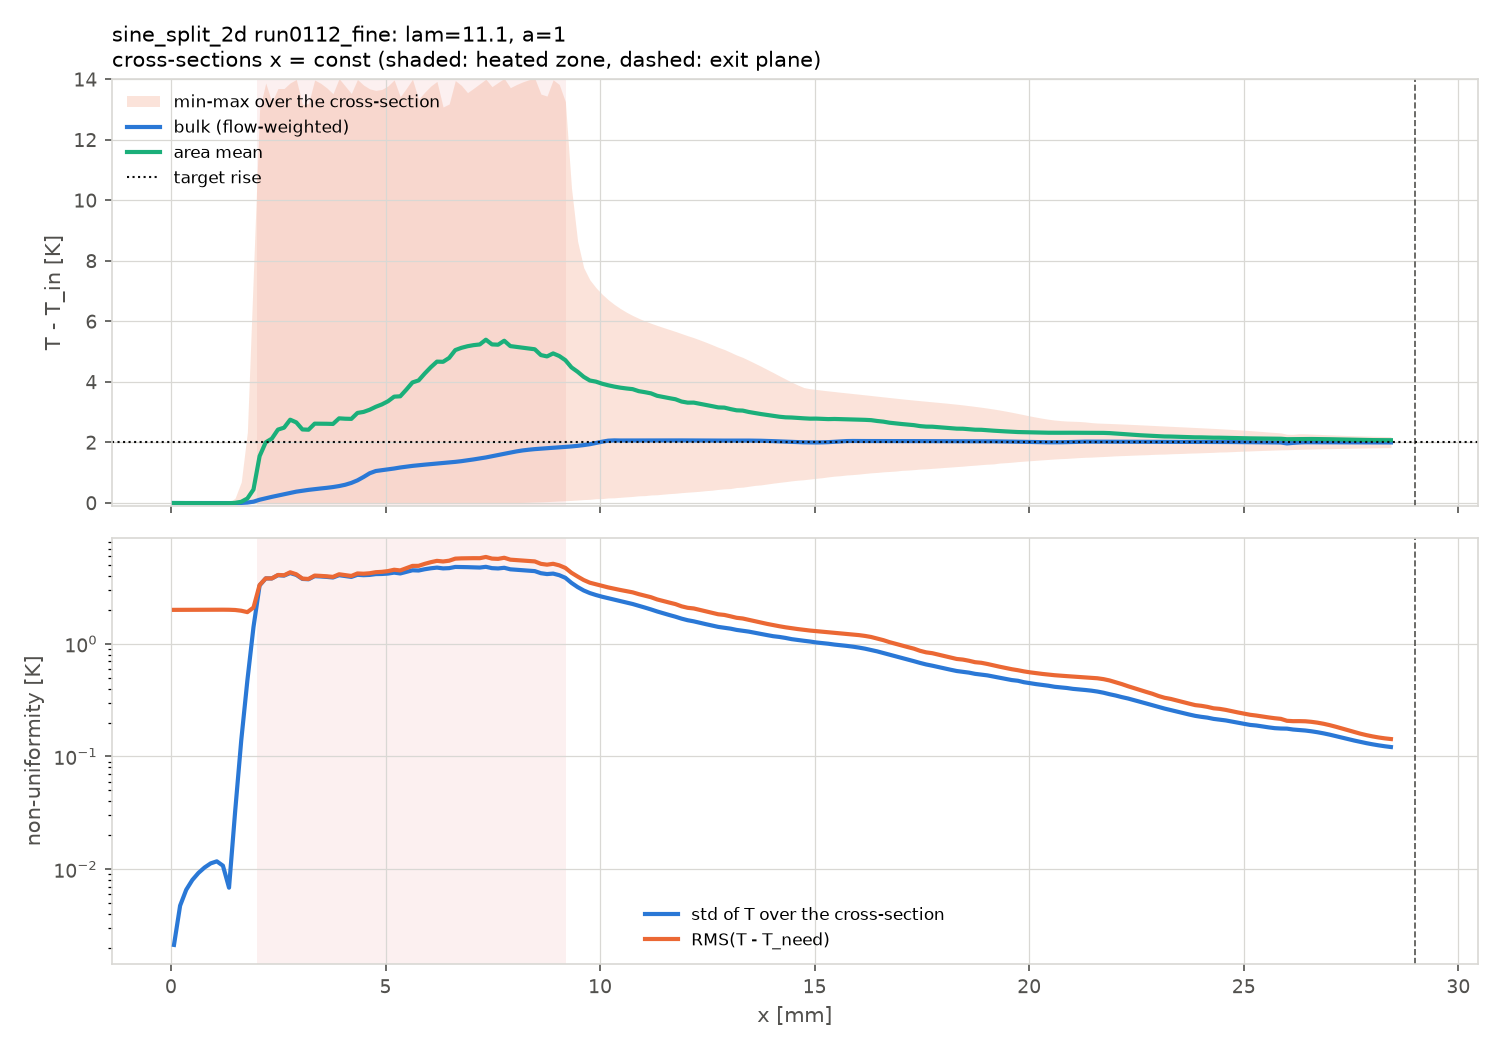
\includegraphics[width=0.8\textwidth,height=0.8\textheight,keepaspectratio]{runs/final_u2d_sine_grid_along_x.png}
\caption{Bulk, mean, min and max temperature along the channel.}
\end{figure}
\begin{figure}[H]\centering
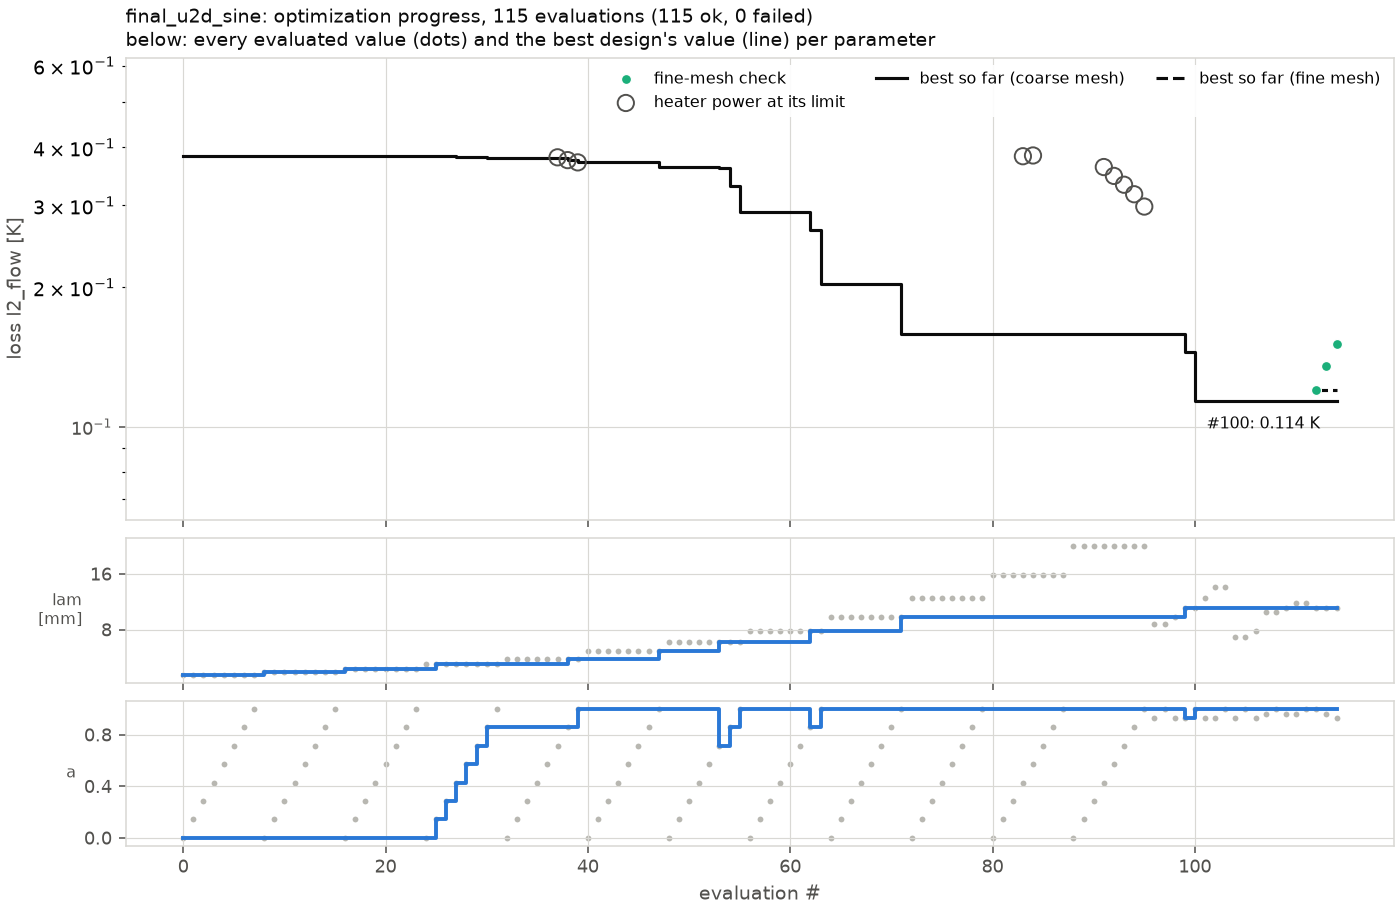
\includegraphics[width=0.85\textwidth]{runs/final_u2d_sine_grid_progress_loss.png}
\caption{Search history: loss of every evaluation, best so far, and the parameters.}
\end{figure}
\clearpage
\subsubsection*{2D serpentine, BO best \#51 ($\lambda$ 8.72, $A$ 3.10, heater 60\,\%): 11.9\mK}
\noindent\texttt{runs/final\_u2d\_serp}\par\medskip
\begin{figure}[H]\centering
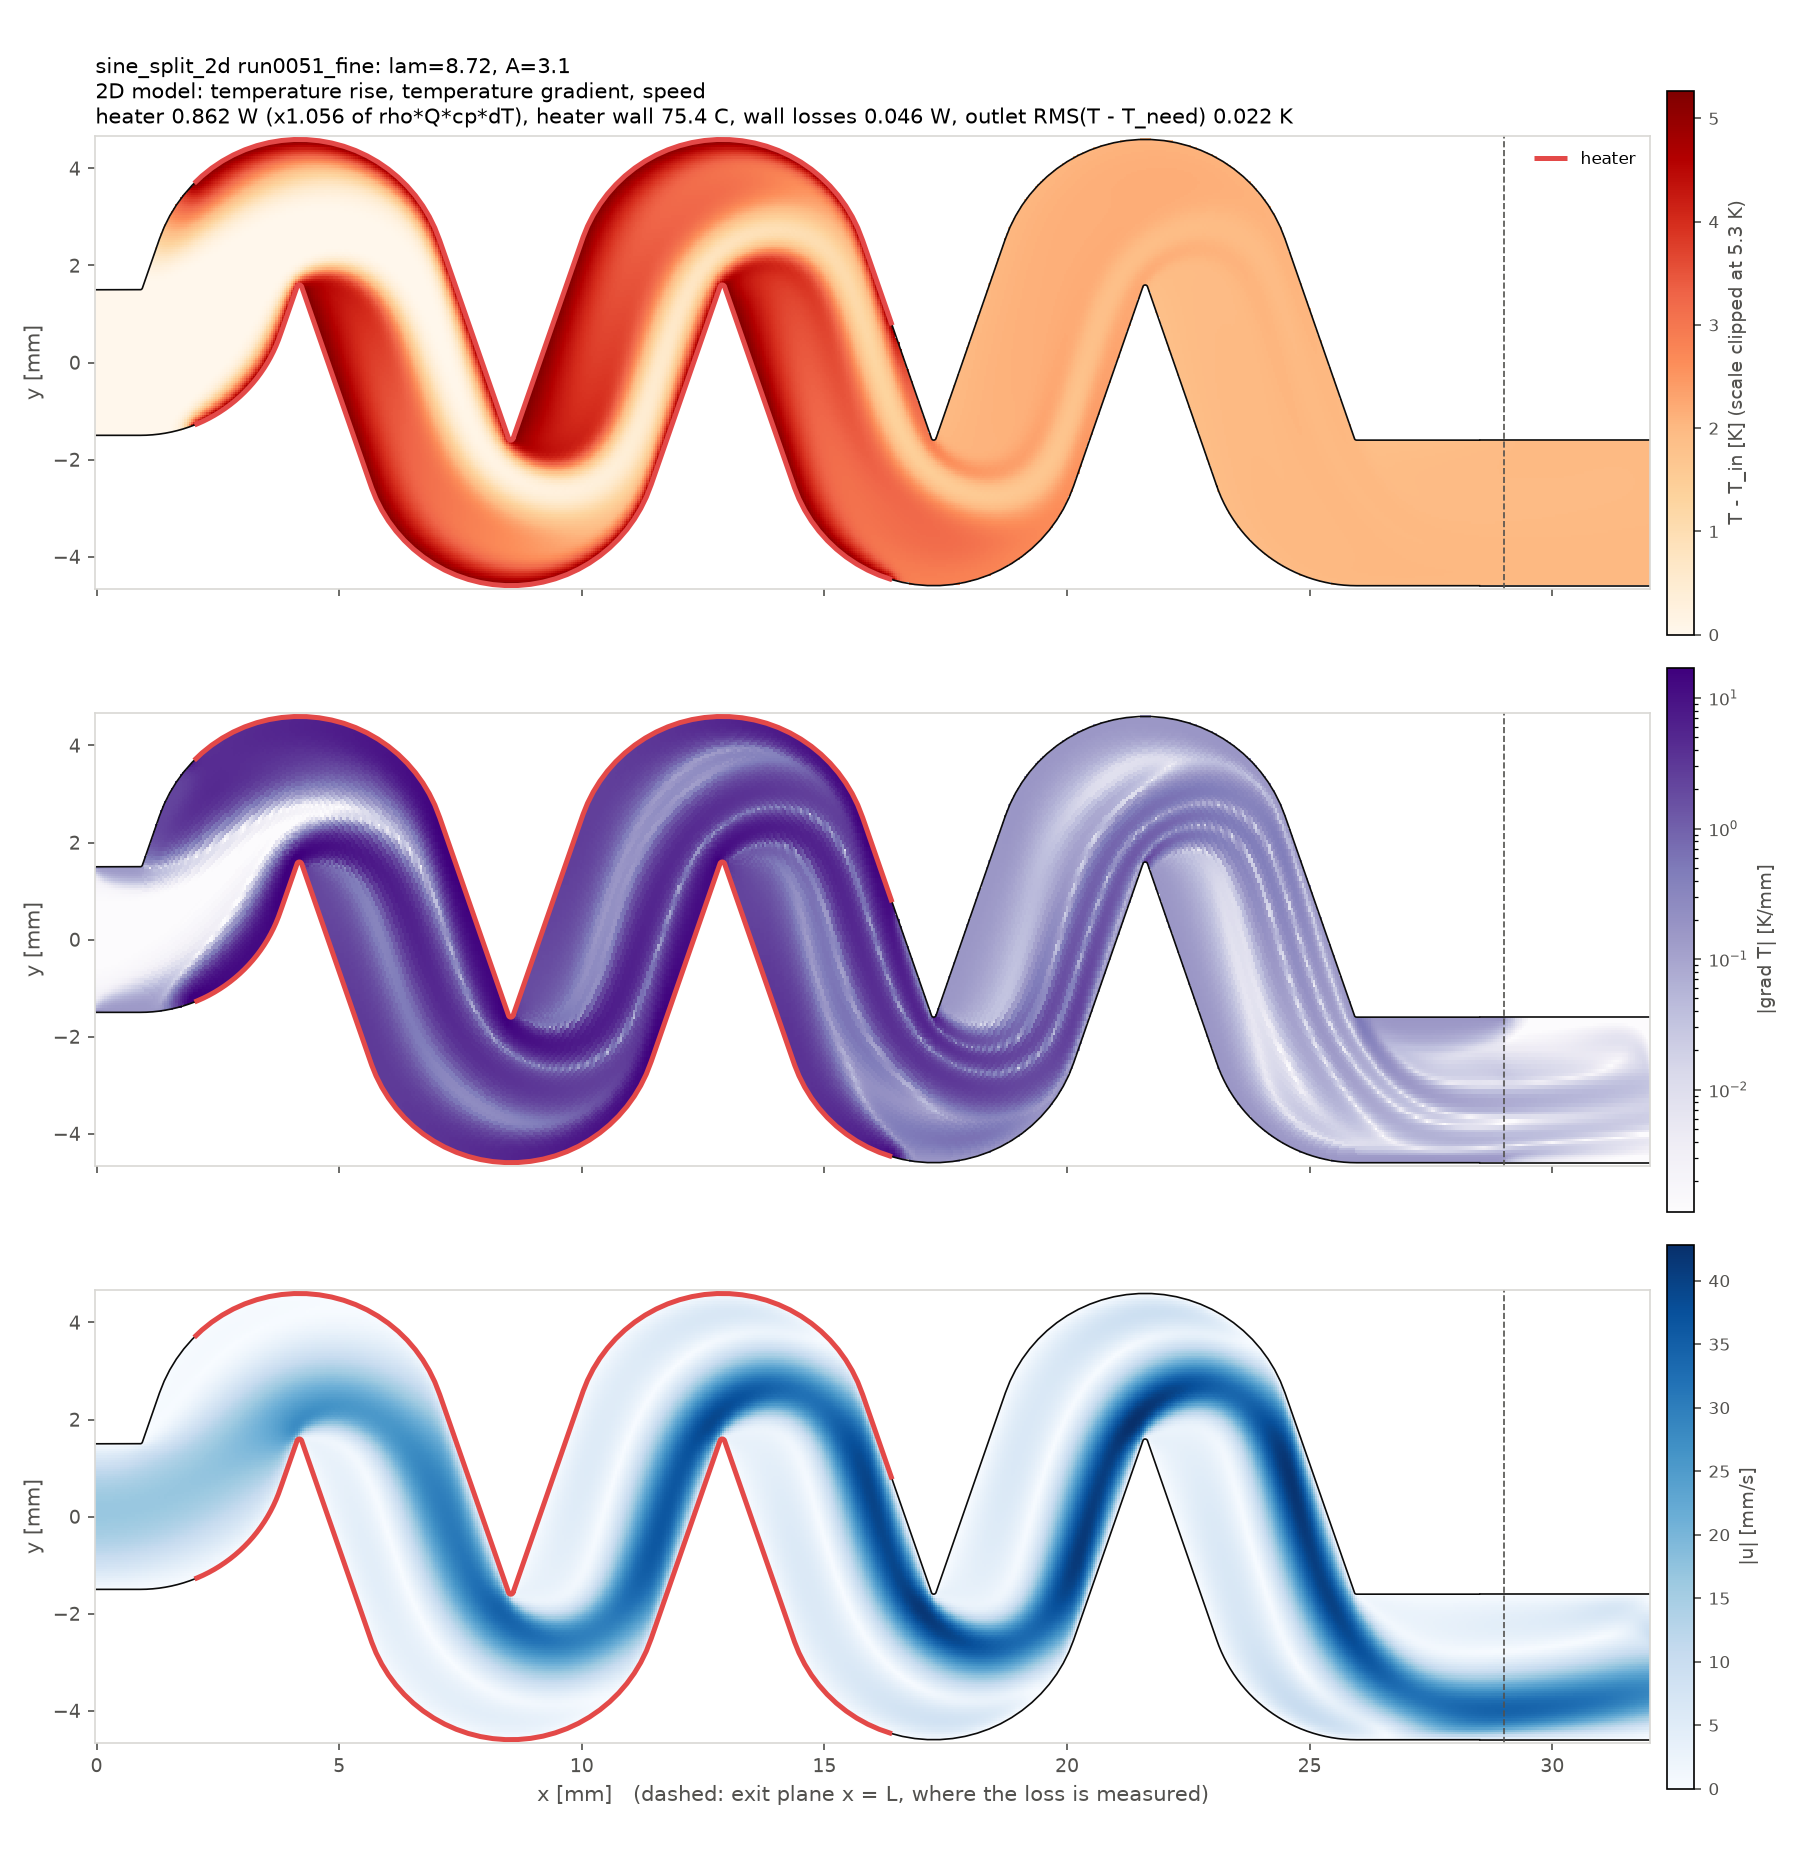
\includegraphics[width=0.95\textwidth,height=0.8\textheight,keepaspectratio]{runs/final_u2d_serp_maps.png}
\caption{Temperature rise, temperature gradient and speed (mid-depth plane in 3D). Red: heated wall. The title's ``outlet RMS'' is the area-weighted $\ell_{2,\mathrm{area}}$.}
\end{figure}
\begin{figure}[H]\centering
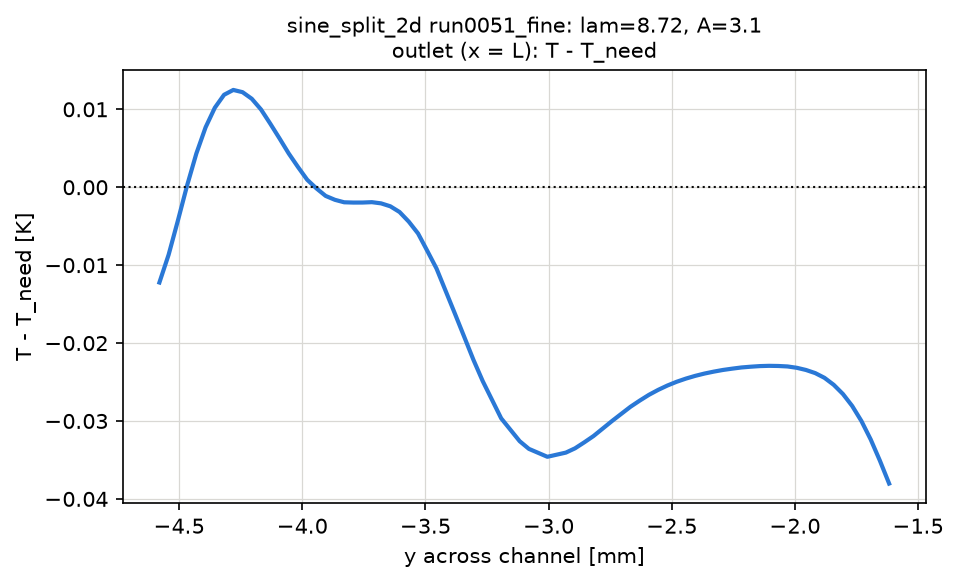
\includegraphics[width=0.75\textwidth,height=0.8\textheight,keepaspectratio]{runs/final_u2d_serp_outlet.png}
\caption{Outlet temperature (and, in 3D, the outlet plane).}
\end{figure}
\begin{figure}[H]\centering
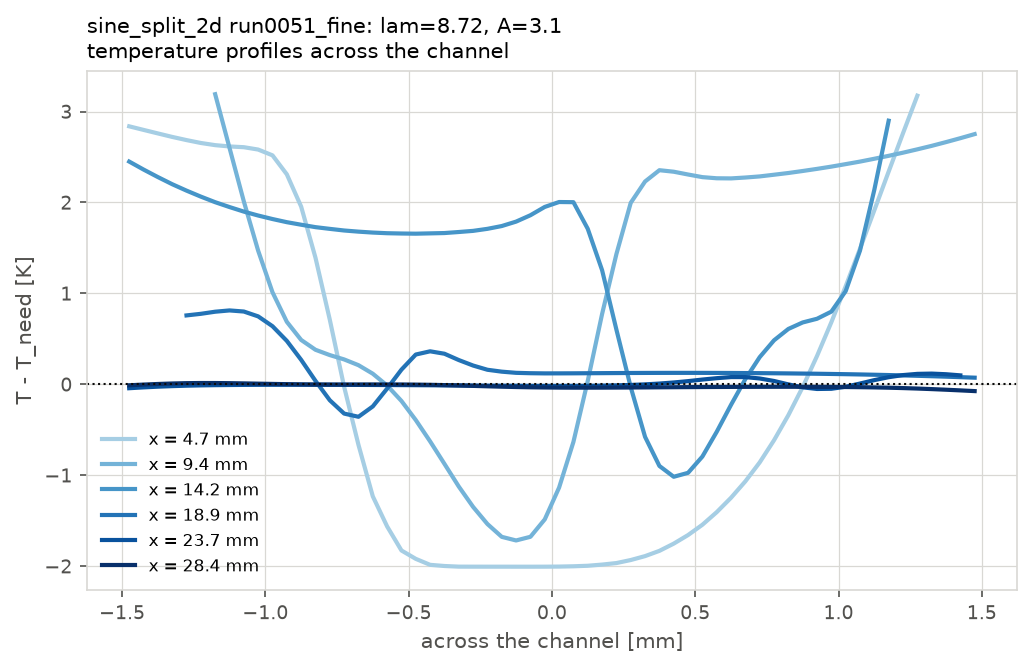
\includegraphics[width=0.62\textwidth,height=0.8\textheight,keepaspectratio]{runs/final_u2d_serp_slices.png}
\caption{Temperature profiles across the channel at several $x$ stations.}
\end{figure}
\begin{figure}[H]\centering
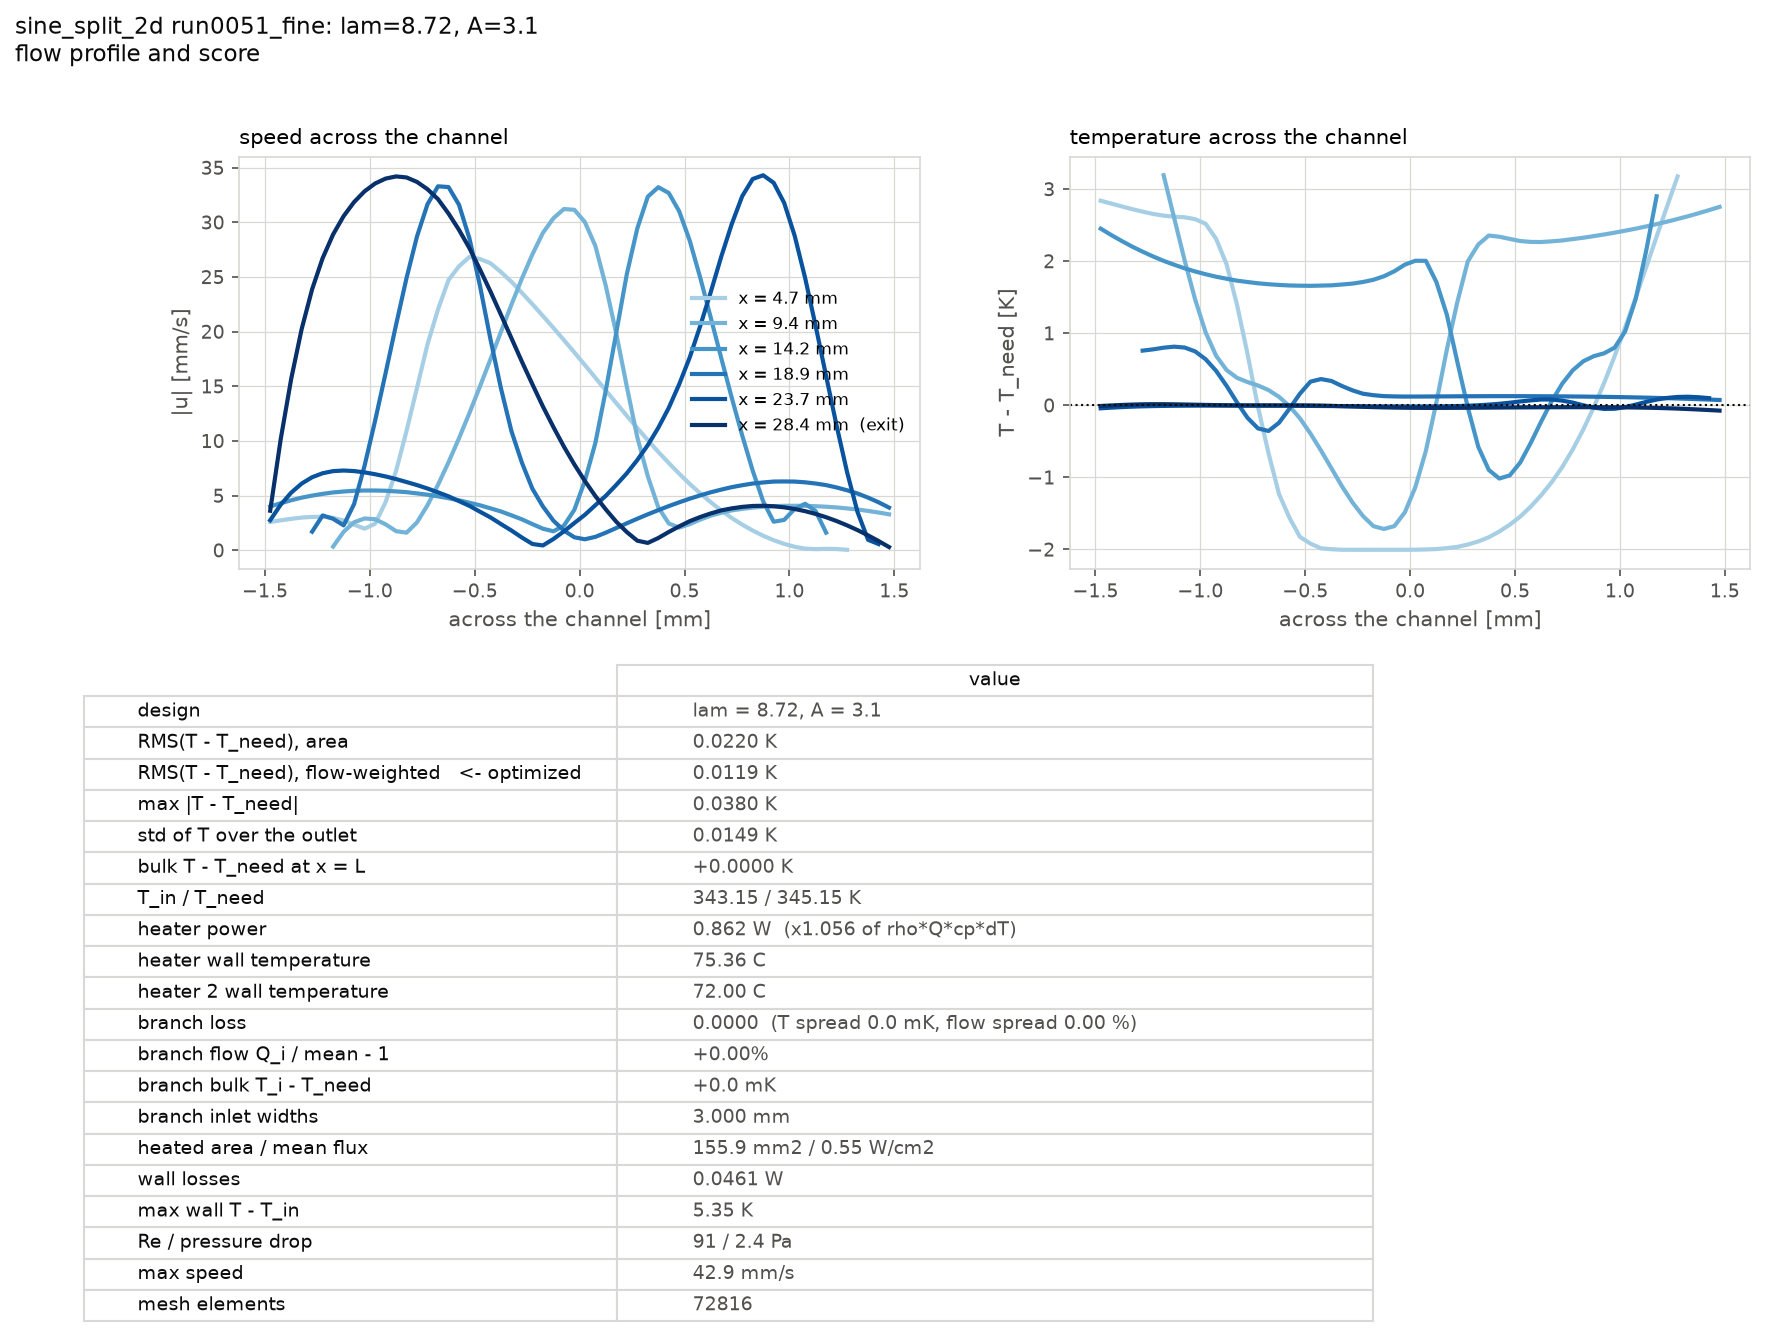
\includegraphics[width=0.8\textwidth,height=0.8\textheight,keepaspectratio]{runs/final_u2d_serp_profile.png}
\caption{Speed and temperature across the channel at several $x$ stations, and the full score table of the design.}
\end{figure}
\begin{figure}[H]\centering
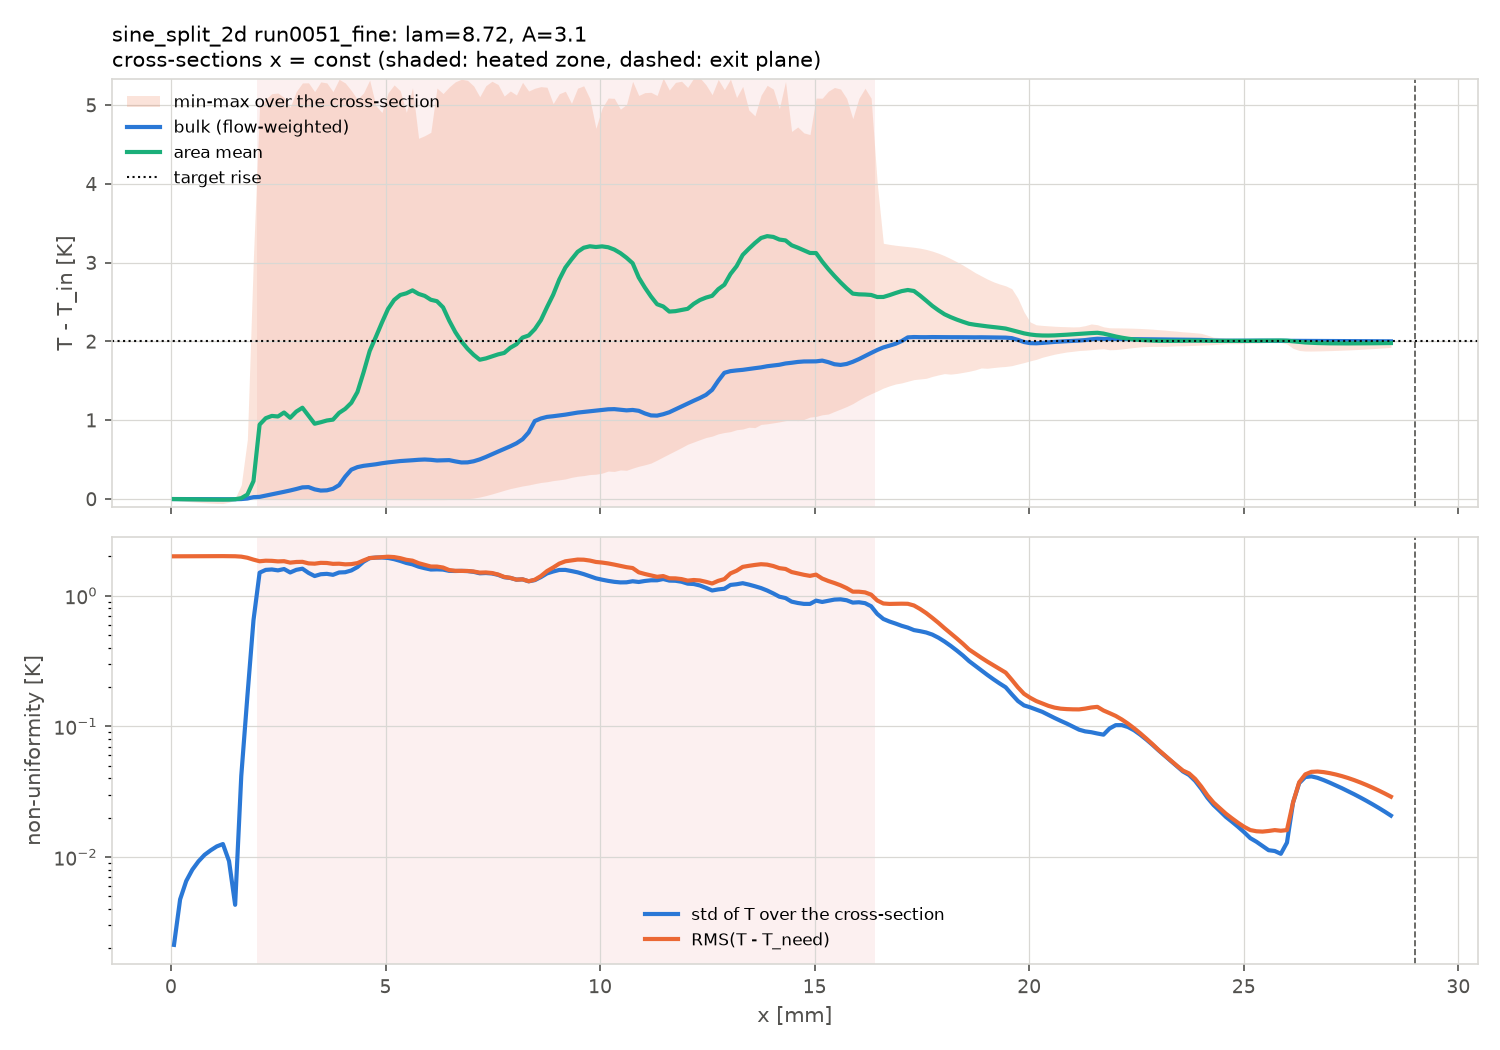
\includegraphics[width=0.8\textwidth,height=0.8\textheight,keepaspectratio]{runs/final_u2d_serp_along_x.png}
\caption{Bulk, mean, min and max temperature along the channel.}
\end{figure}
\begin{figure}[H]\centering
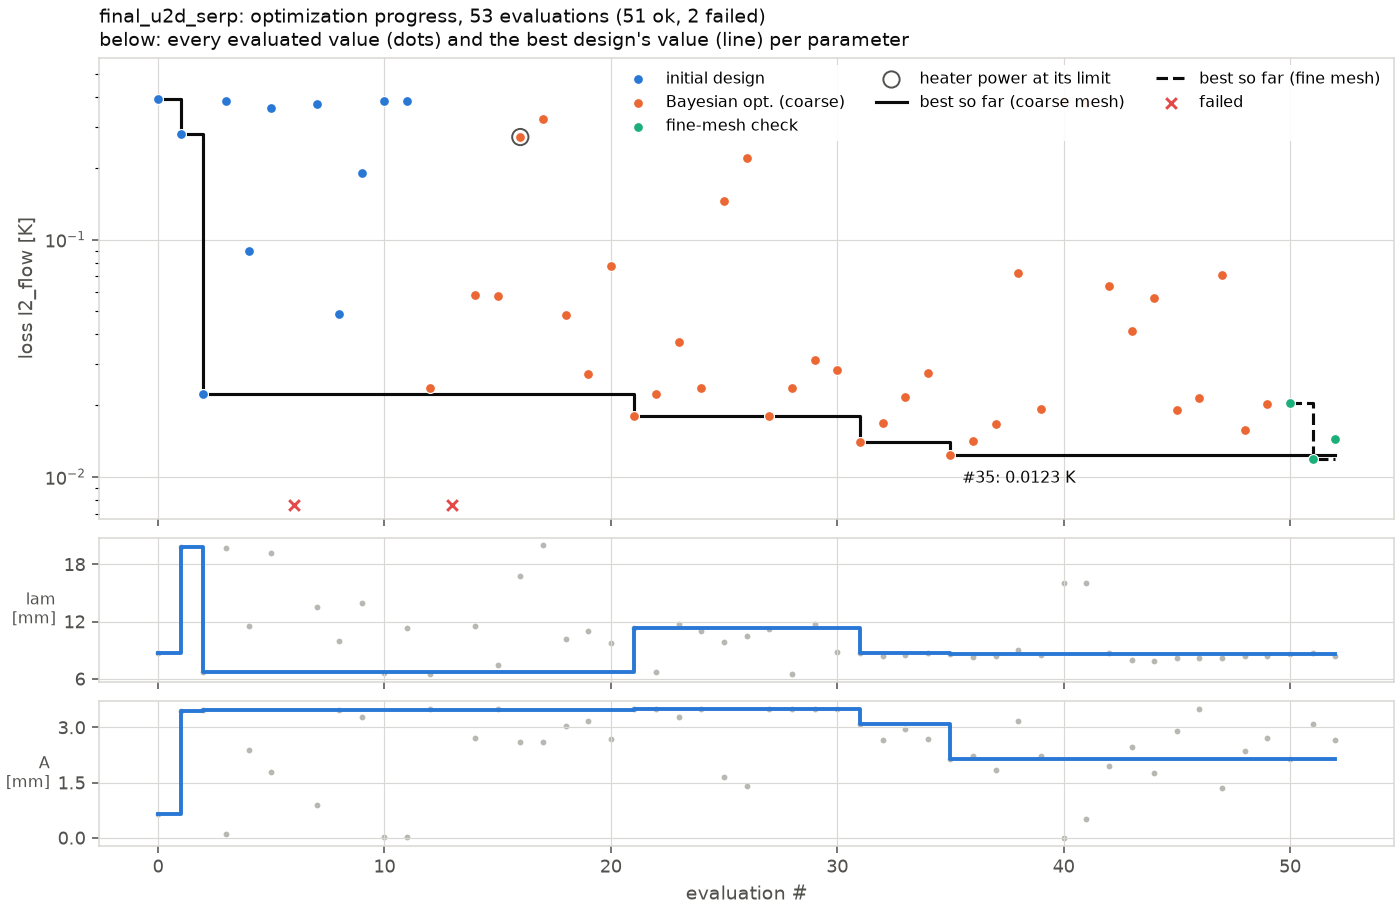
\includegraphics[width=0.85\textwidth]{runs/final_u2d_serp_progress_loss.png}
\caption{Search history: loss of every evaluation, best so far, and the parameters.}
\end{figure}
\clearpage
\subsubsection*{2D serpentine, grid best \#108 ($\lambda$ 8.34, $A$ 2.13, heater 40\,\%): 6.3\mK}
\noindent\texttt{runs/final\_u2d\_serp\_grid}\par\medskip
\begin{figure}[H]\centering
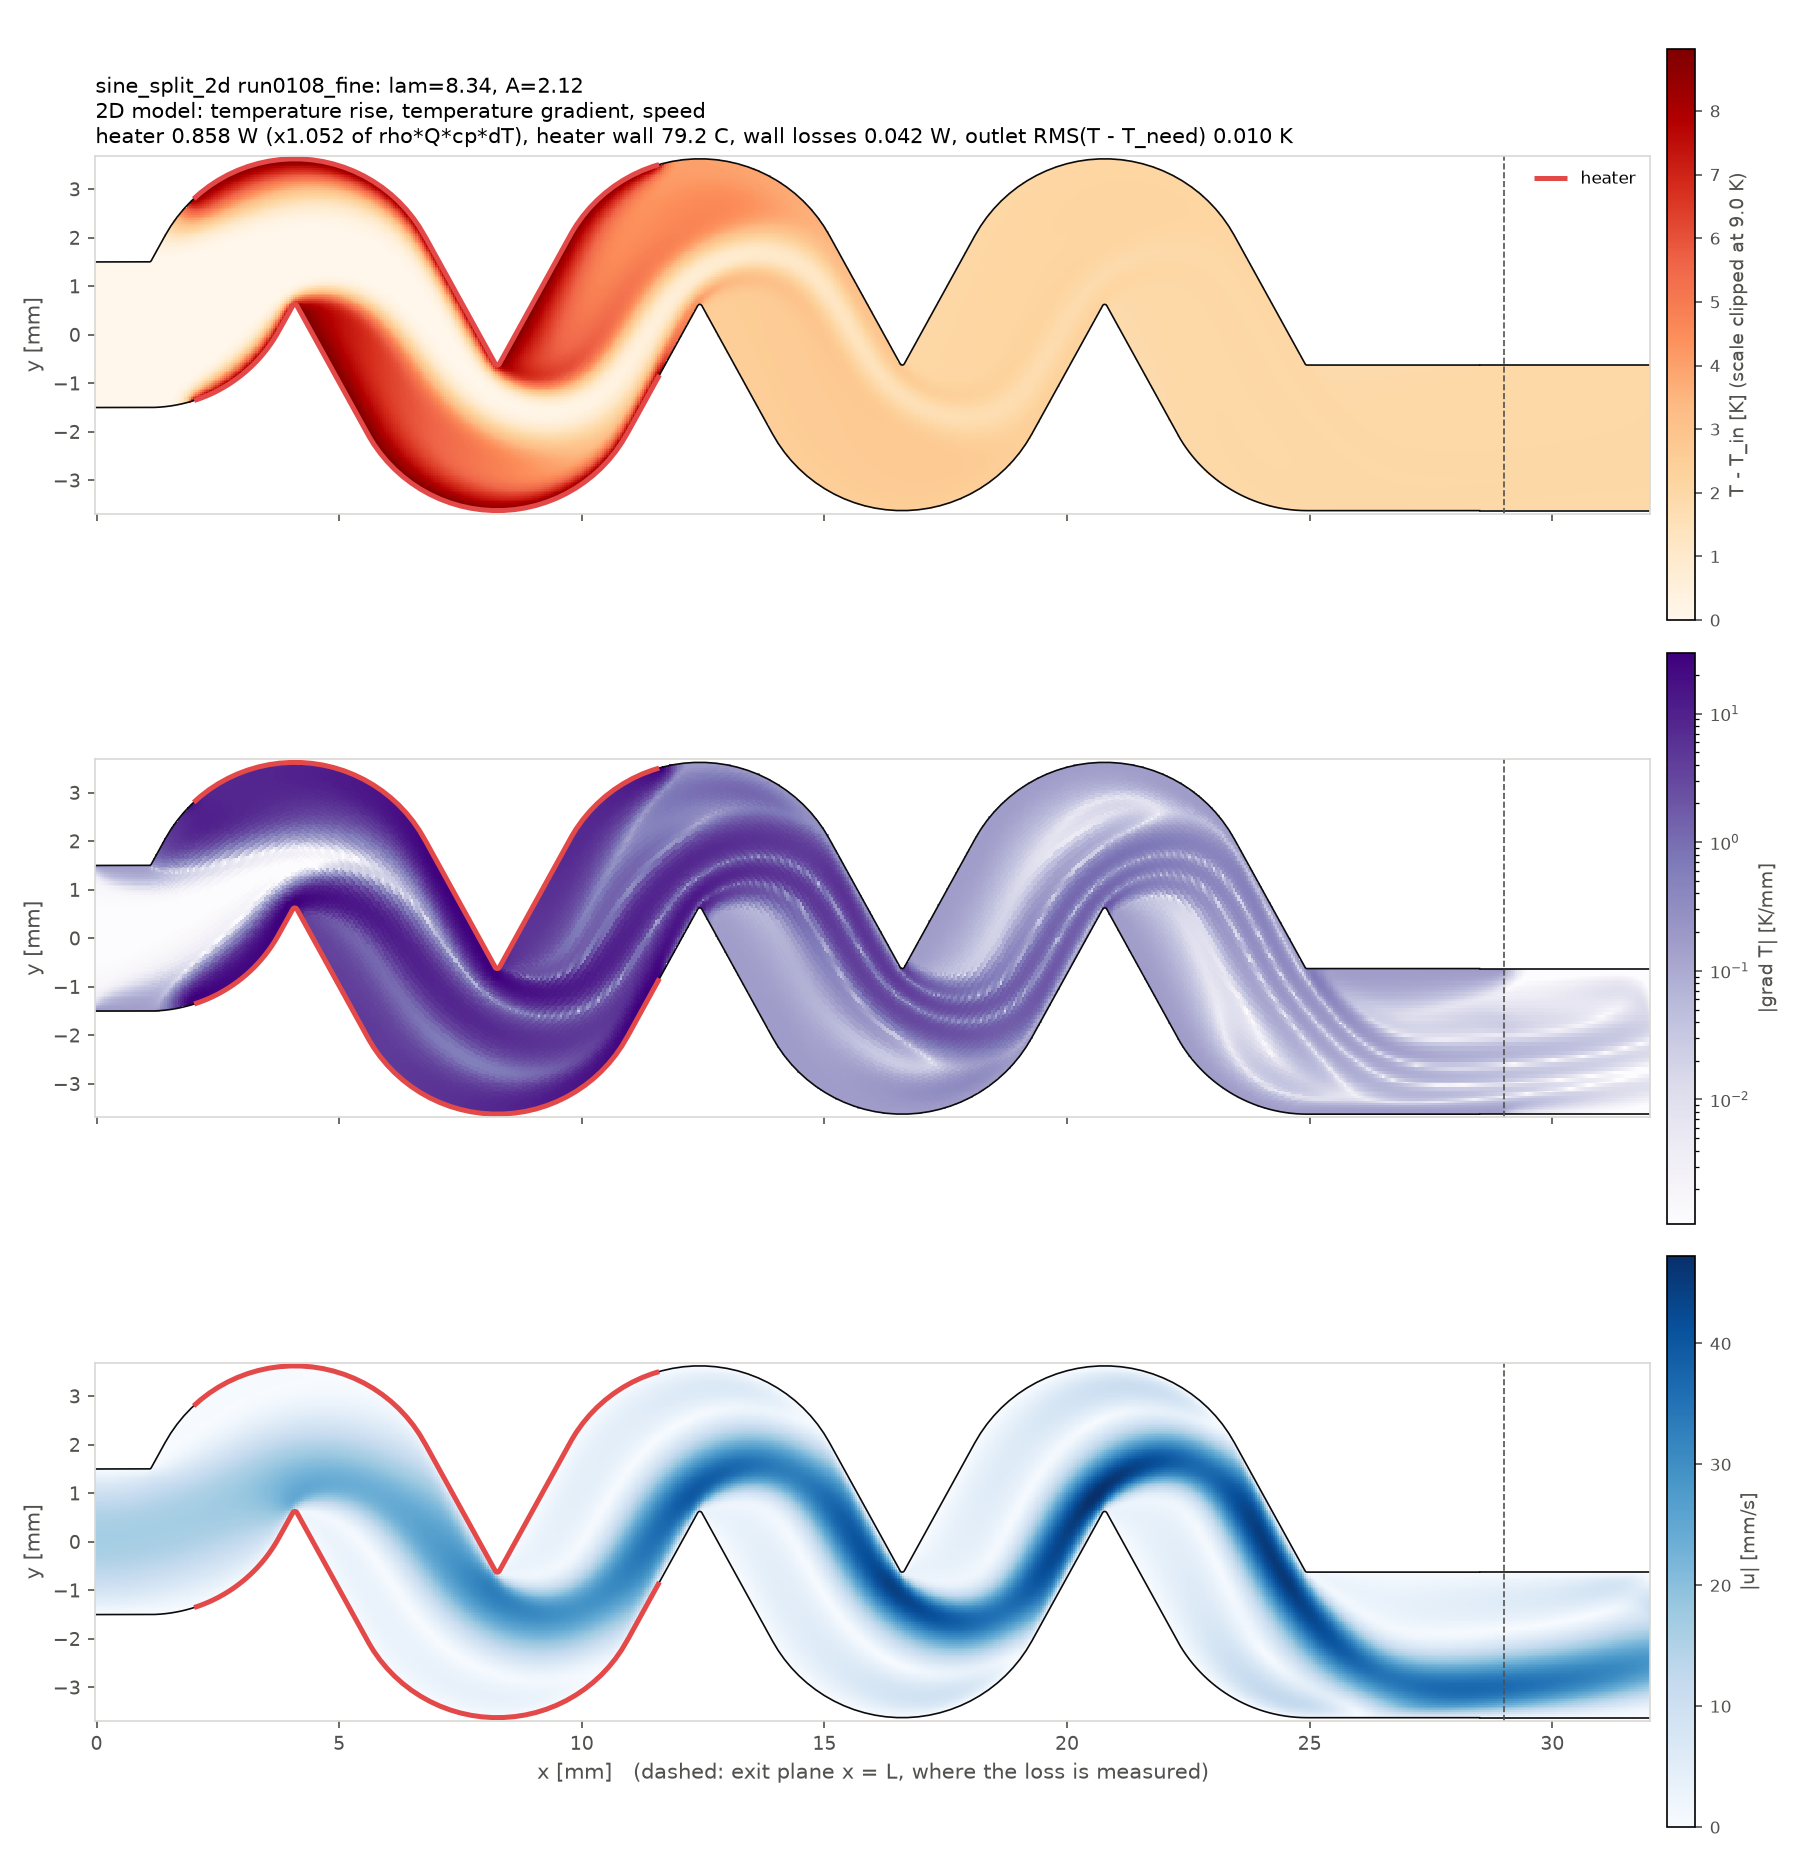
\includegraphics[width=0.95\textwidth,height=0.8\textheight,keepaspectratio]{runs/final_u2d_serp_grid_maps.png}
\caption{Temperature rise, temperature gradient and speed (mid-depth plane in 3D). Red: heated wall. The title's ``outlet RMS'' is the area-weighted $\ell_{2,\mathrm{area}}$.}
\end{figure}
\begin{figure}[H]\centering
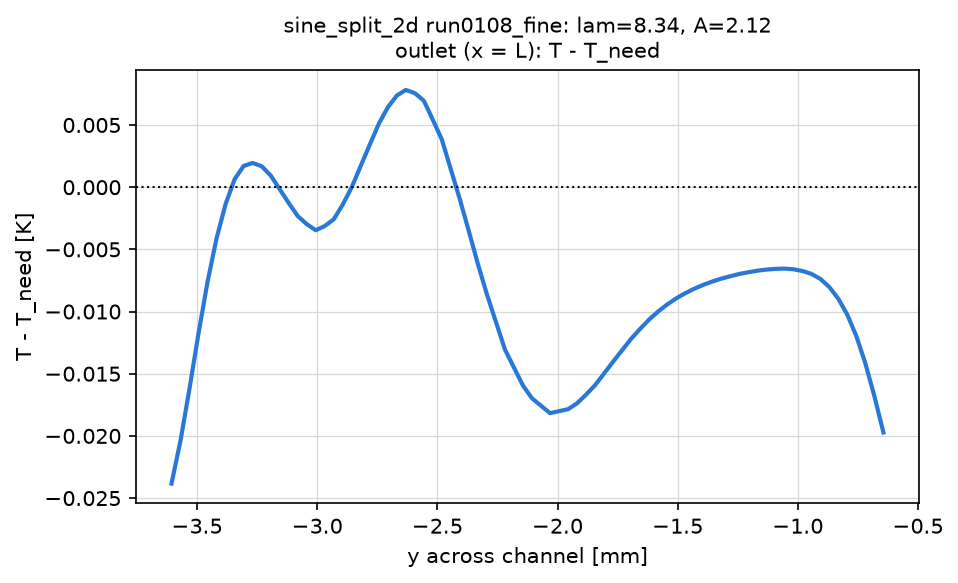
\includegraphics[width=0.75\textwidth,height=0.8\textheight,keepaspectratio]{runs/final_u2d_serp_grid_outlet.png}
\caption{Outlet temperature (and, in 3D, the outlet plane).}
\end{figure}
\begin{figure}[H]\centering
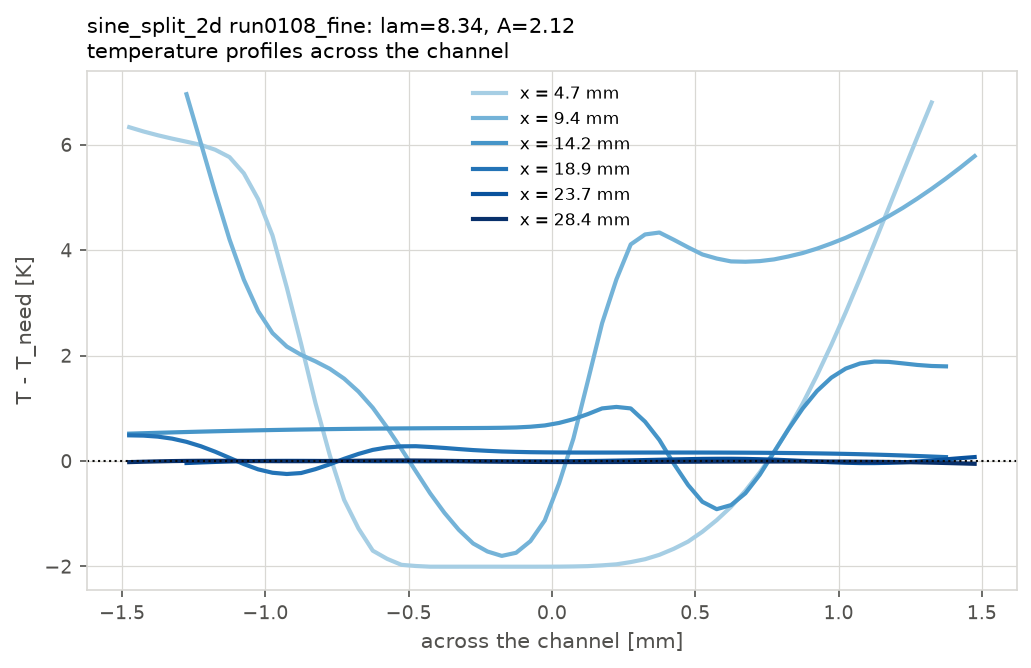
\includegraphics[width=0.62\textwidth,height=0.8\textheight,keepaspectratio]{runs/final_u2d_serp_grid_slices.png}
\caption{Temperature profiles across the channel at several $x$ stations.}
\end{figure}
\begin{figure}[H]\centering
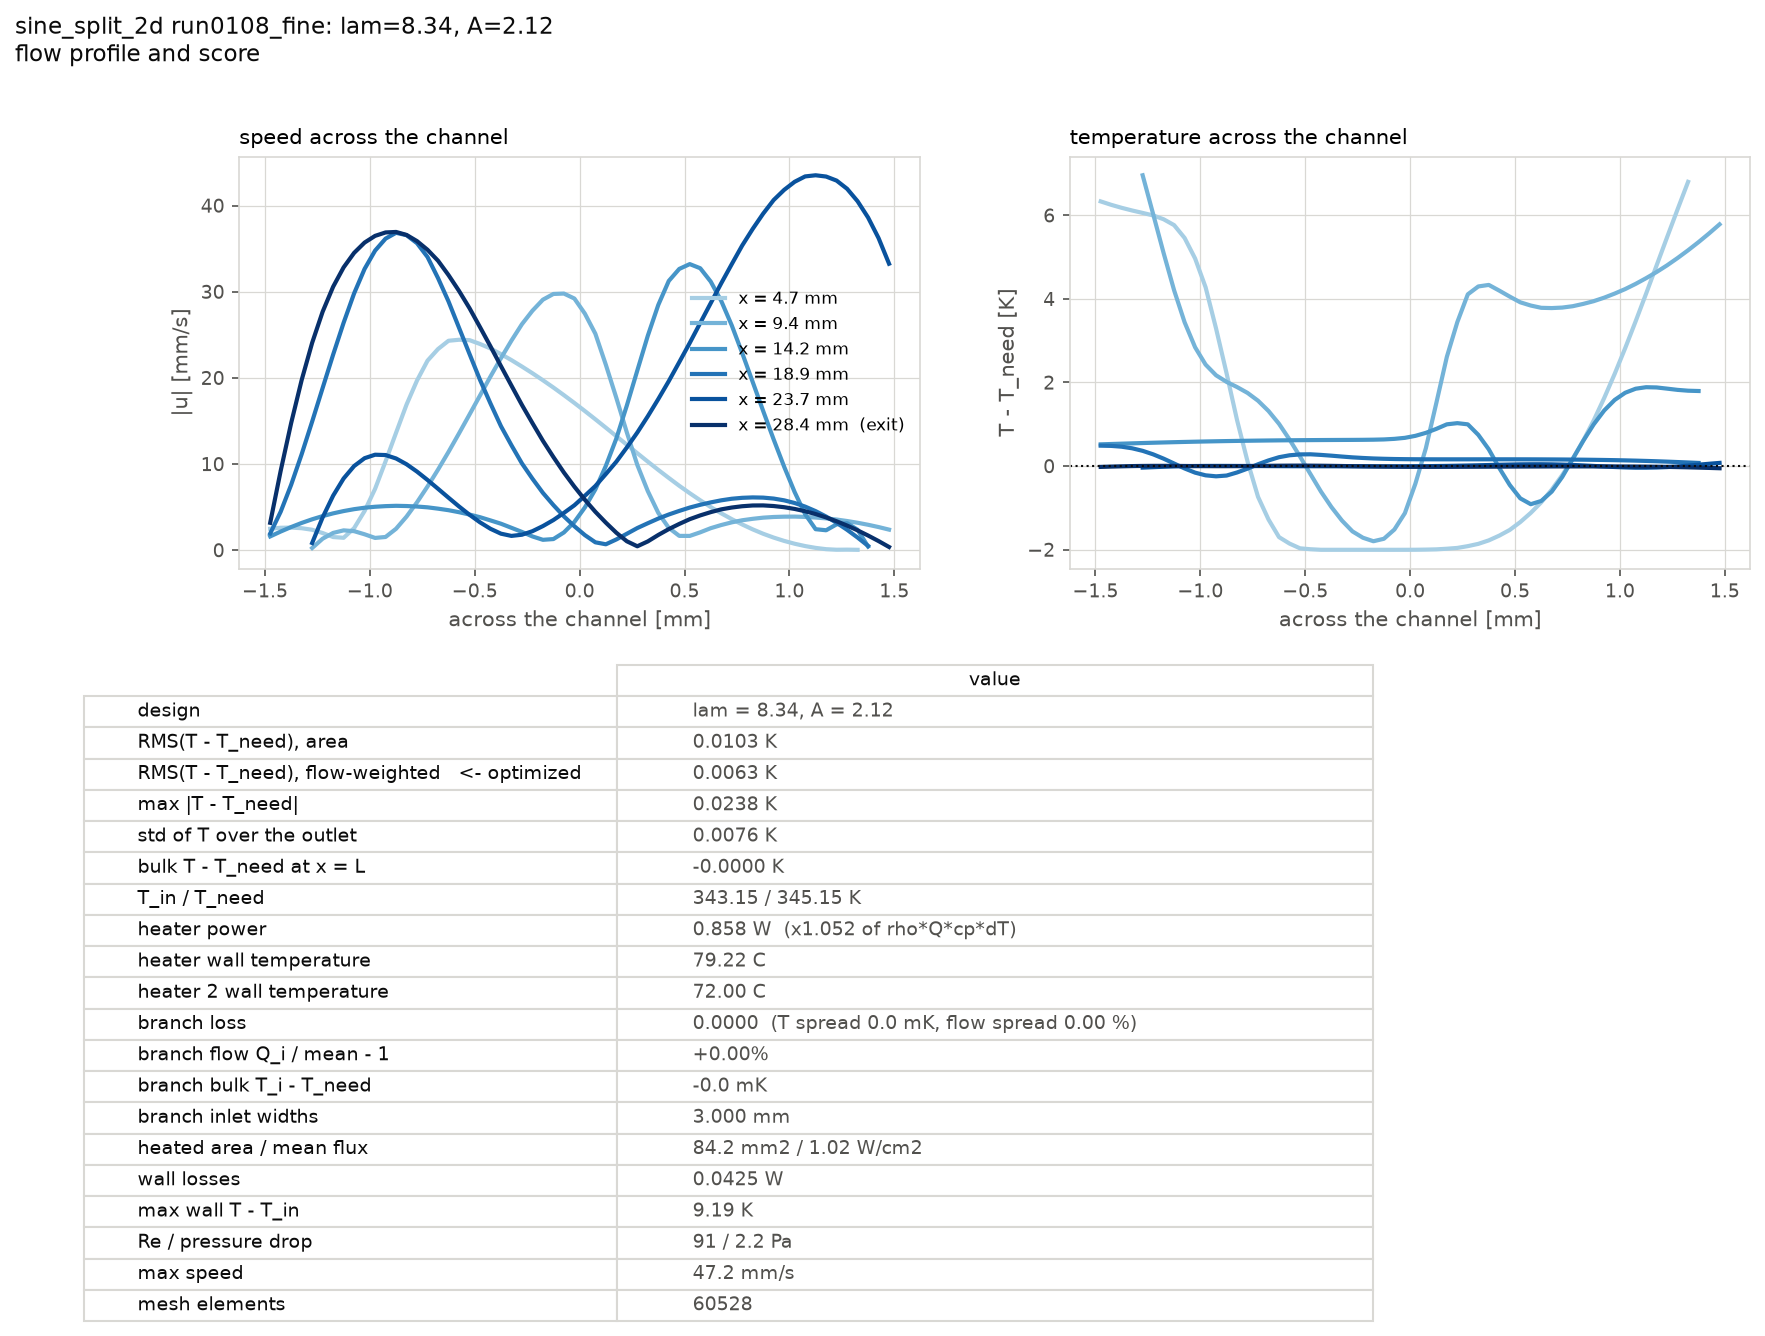
\includegraphics[width=0.8\textwidth,height=0.8\textheight,keepaspectratio]{runs/final_u2d_serp_grid_profile.png}
\caption{Speed and temperature across the channel at several $x$ stations, and the full score table of the design.}
\end{figure}
\begin{figure}[H]\centering
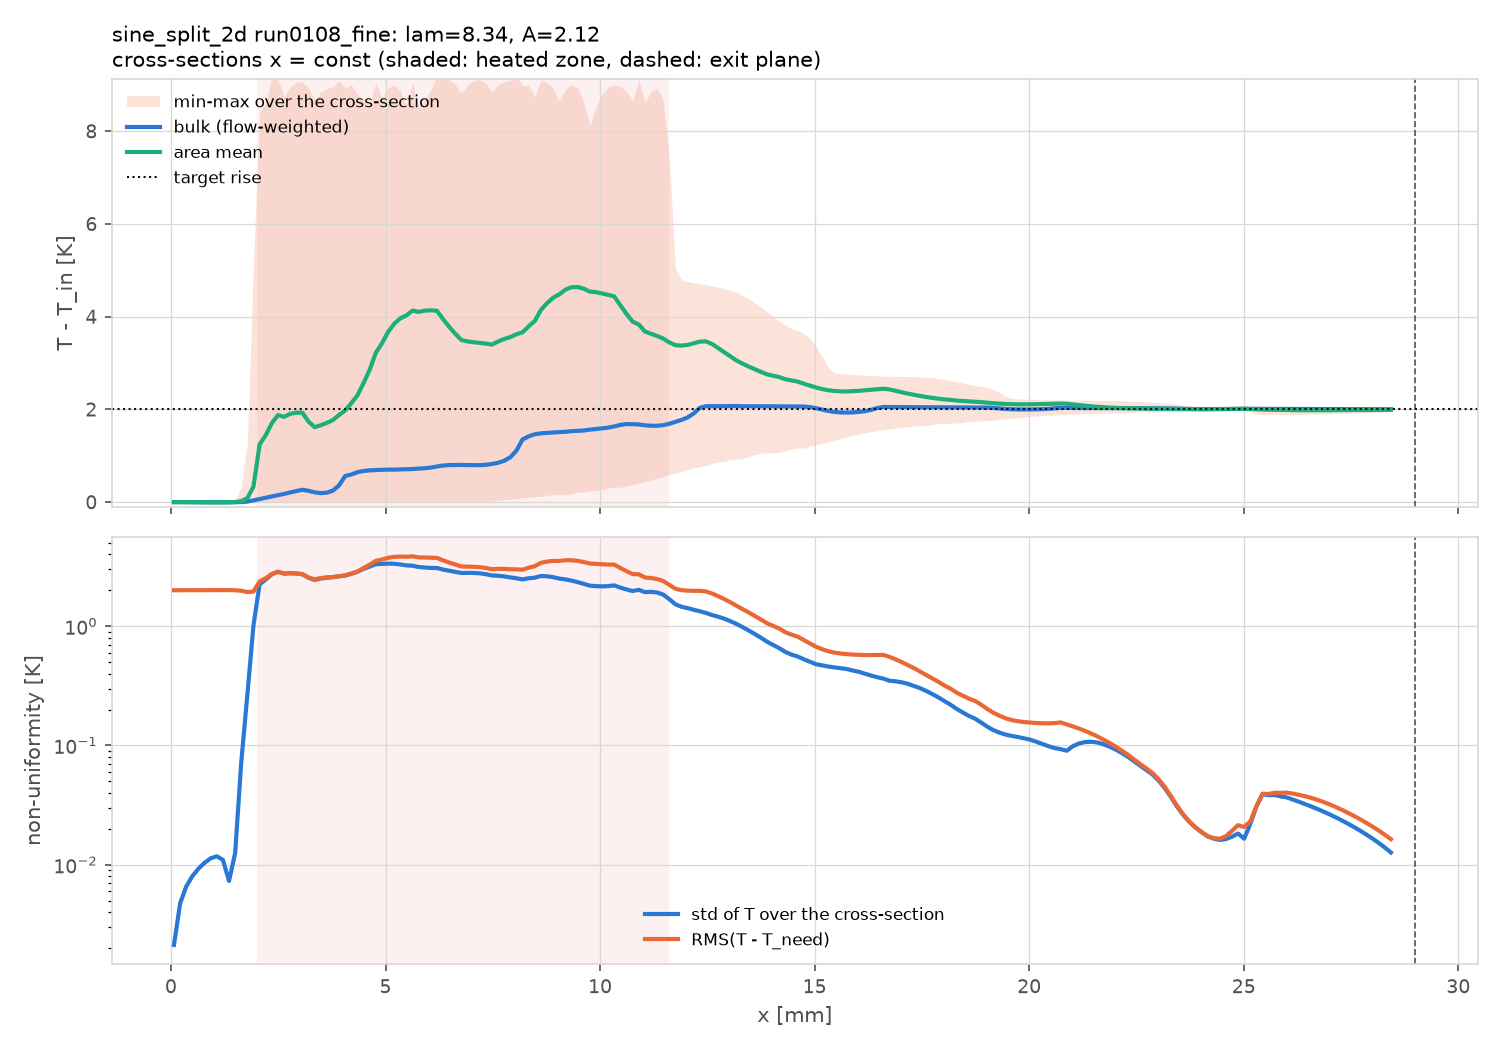
\includegraphics[width=0.8\textwidth,height=0.8\textheight,keepaspectratio]{runs/final_u2d_serp_grid_along_x.png}
\caption{Bulk, mean, min and max temperature along the channel.}
\end{figure}
\begin{figure}[H]\centering
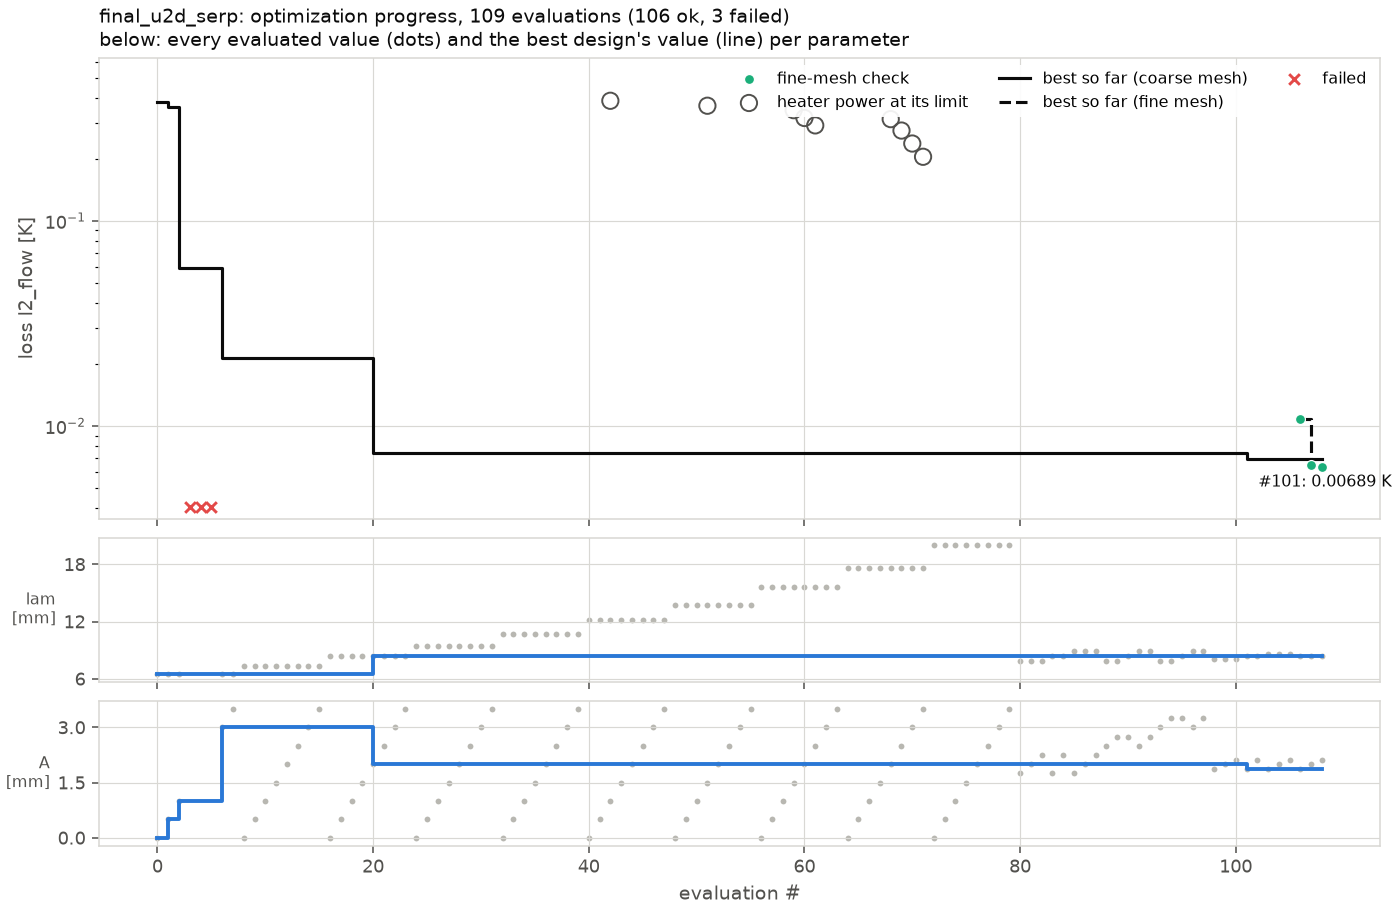
\includegraphics[width=0.85\textwidth]{runs/final_u2d_serp_grid_progress_loss.png}
\caption{Search history: loss of every evaluation, best so far, and the parameters.}
\end{figure}
\subsection{One outlet, 3D (depth 3\,mm)}
\clearpage
\subsubsection*{3D straight reference, fully heated (heater on all four walls, 24\mm)}
\noindent\texttt{runs/final\_u3d\_straight\_ref\_single}\par\medskip
\begin{figure}[H]\centering
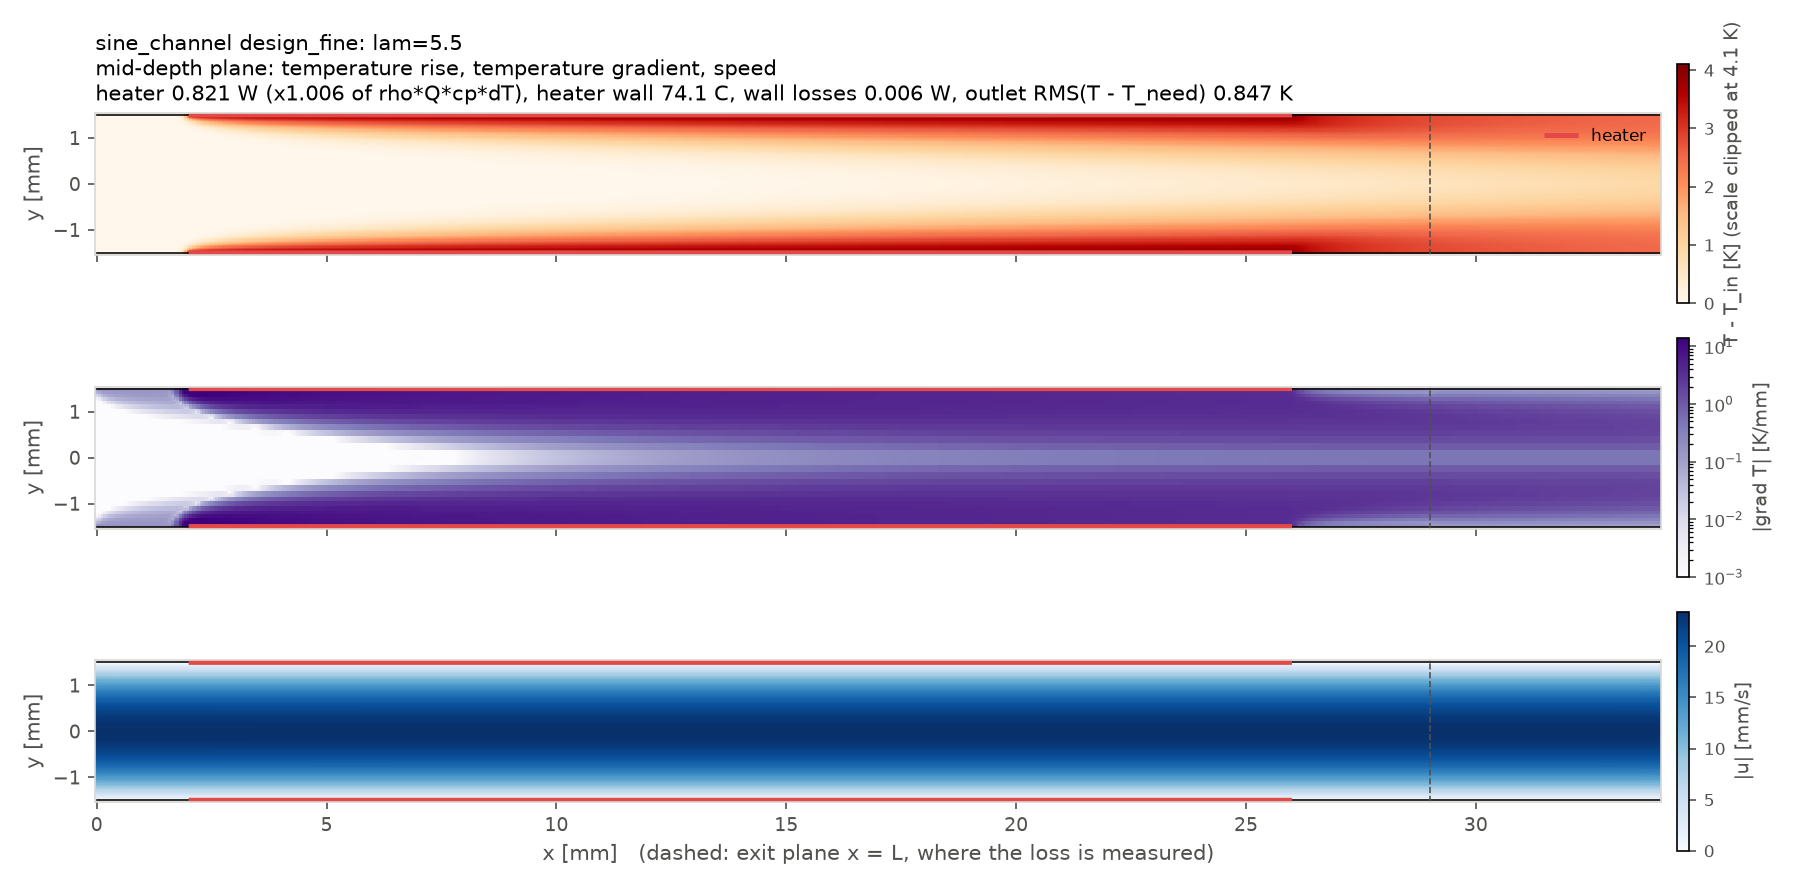
\includegraphics[width=0.95\textwidth,height=0.8\textheight,keepaspectratio]{runs/final_u3d_straight_ref_single_maps.png}
\caption{Temperature rise, temperature gradient and speed (mid-depth plane in 3D). Red: heated wall. The title's ``outlet RMS'' is the area-weighted $\ell_{2,\mathrm{area}}$.}
\end{figure}
\begin{figure}[H]\centering
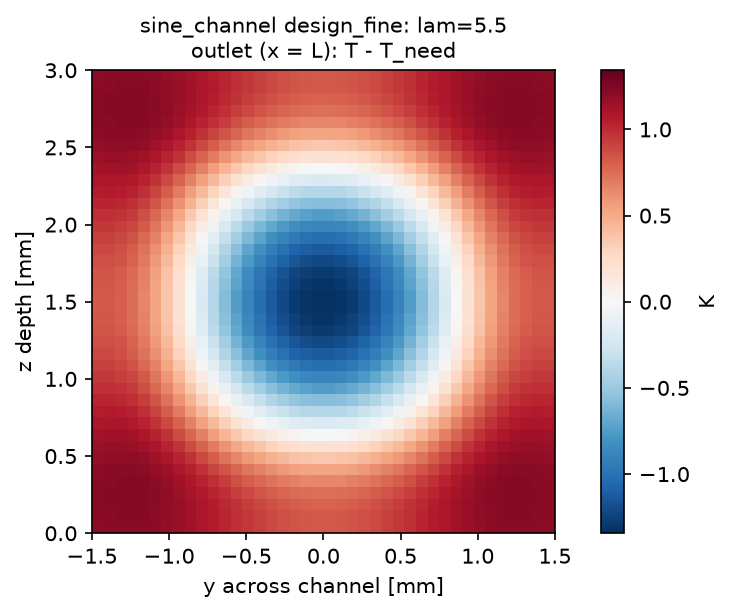
\includegraphics[width=0.75\textwidth,height=0.8\textheight,keepaspectratio]{runs/final_u3d_straight_ref_single_outlet.png}
\caption{Outlet temperature (and, in 3D, the outlet plane).}
\end{figure}
\begin{figure}[H]\centering
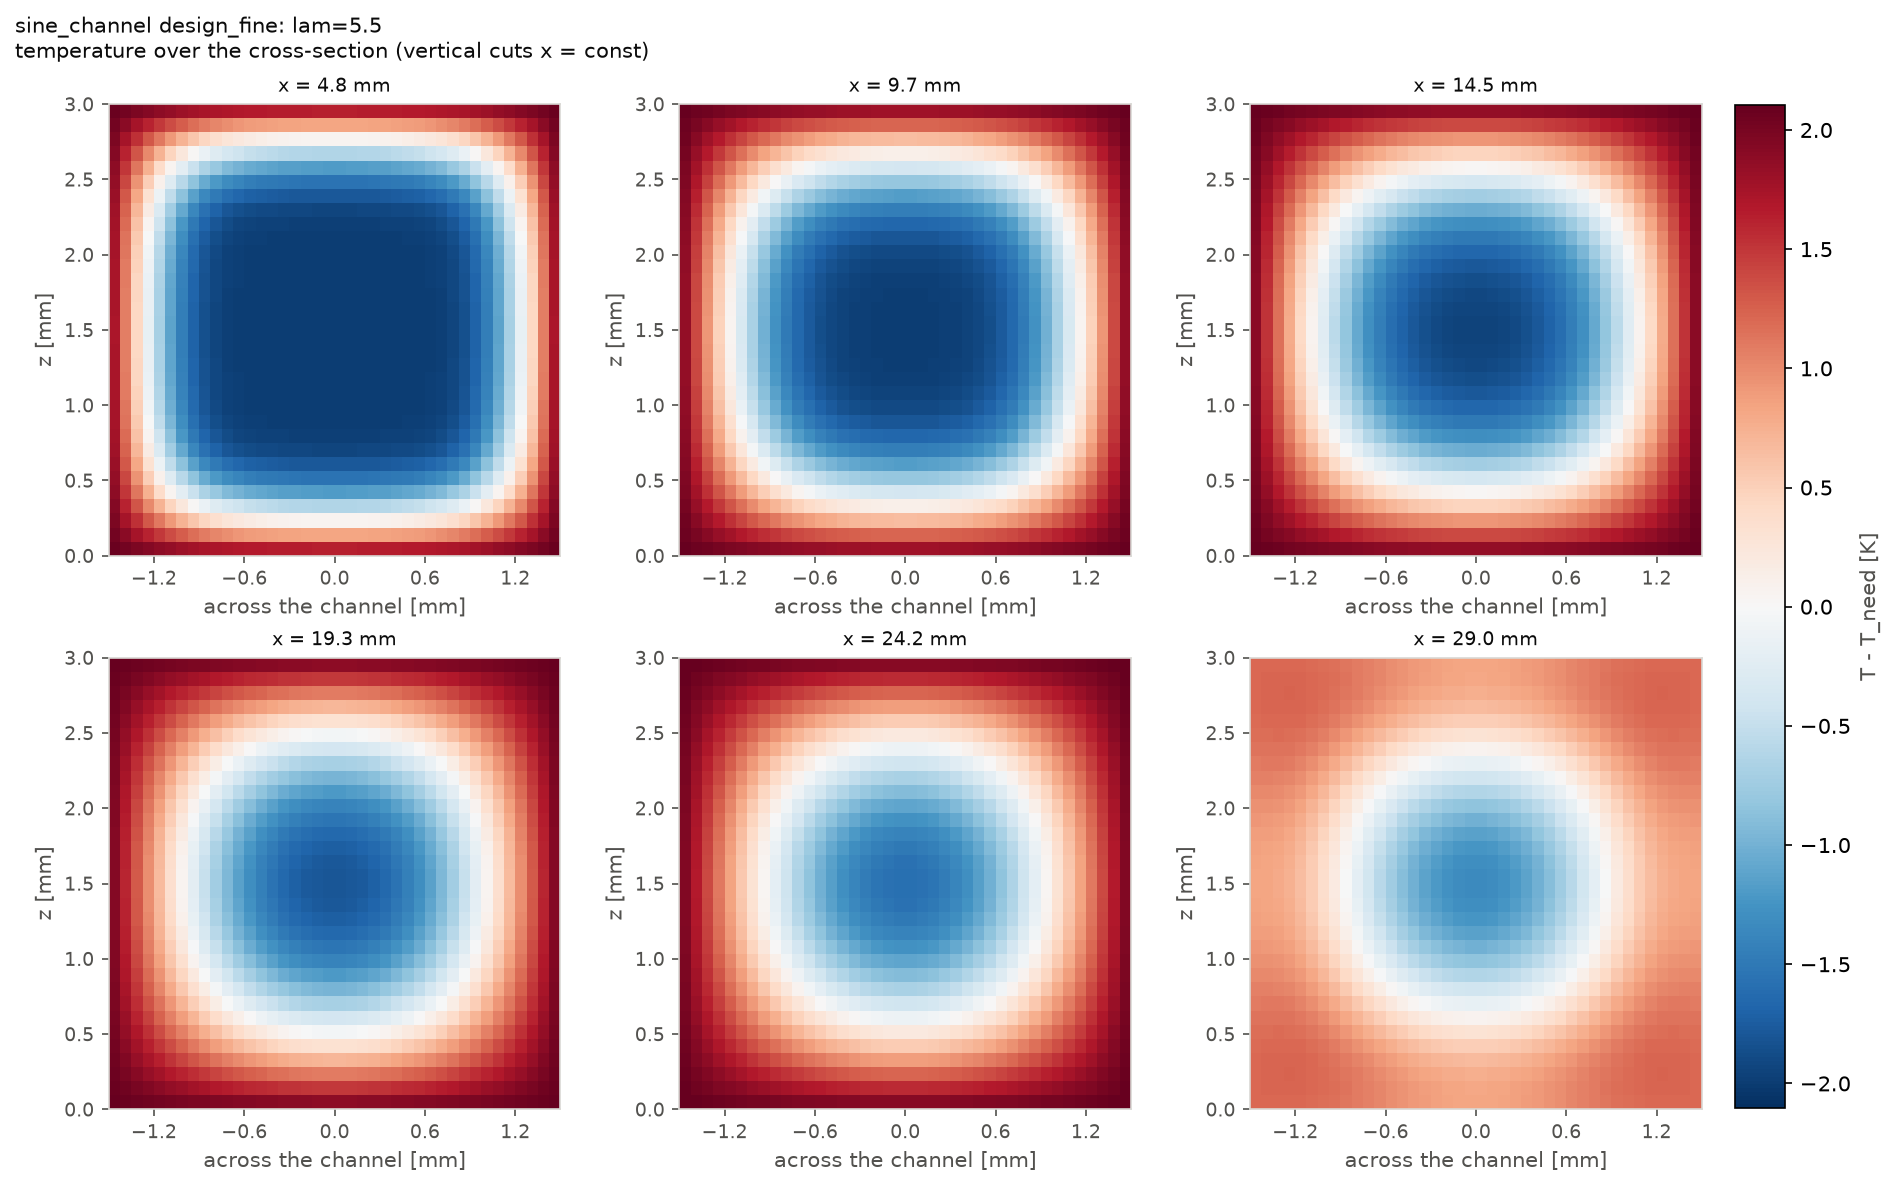
\includegraphics[width=0.62\textwidth,height=0.8\textheight,keepaspectratio]{runs/final_u3d_straight_ref_single_slices.png}
\caption{Temperature profiles across the channel at several $x$ stations.}
\end{figure}
\begin{figure}[H]\centering
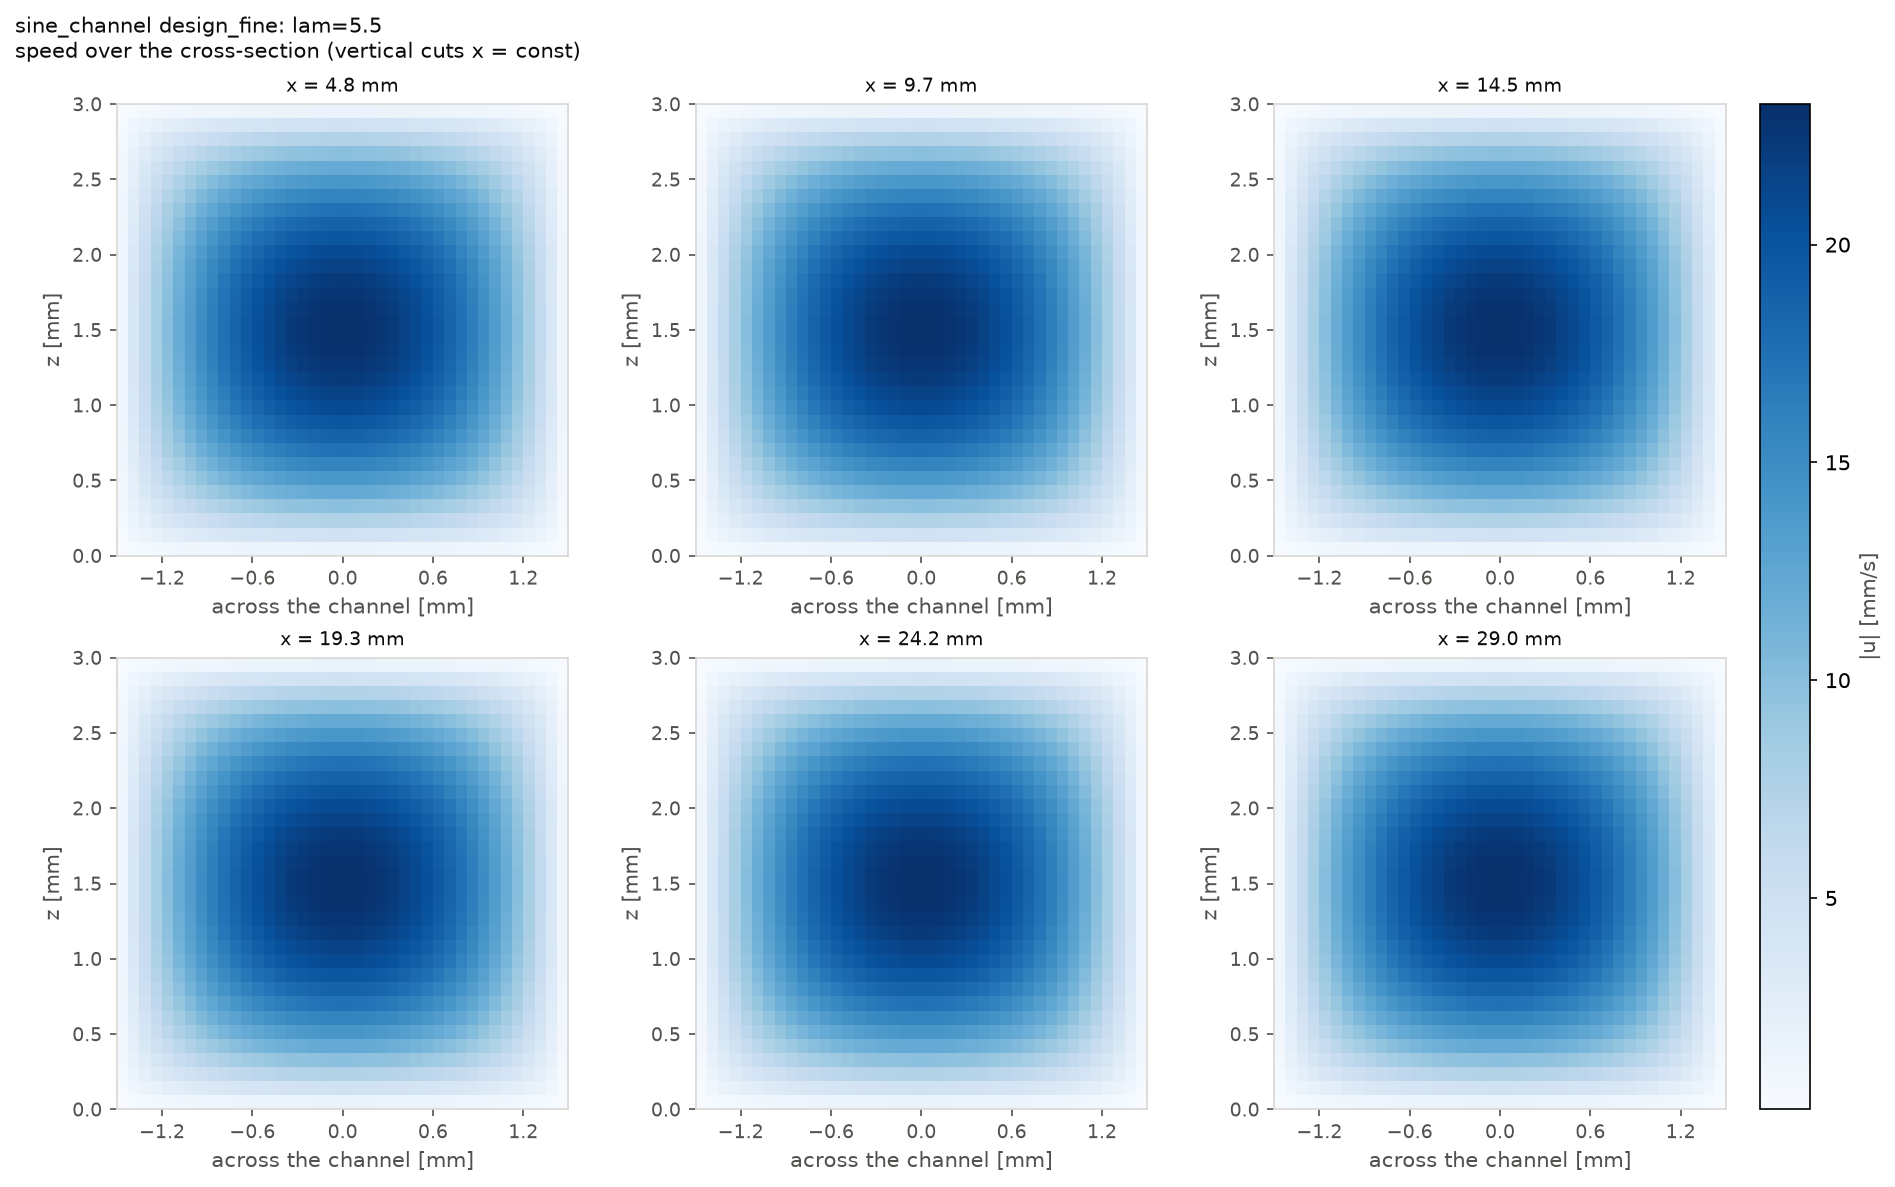
\includegraphics[width=0.85\textwidth,height=0.8\textheight,keepaspectratio]{runs/final_u3d_straight_ref_single_slices_u.png}
\caption{Velocity on cross-sections (3D).}
\end{figure}
\begin{figure}[H]\centering
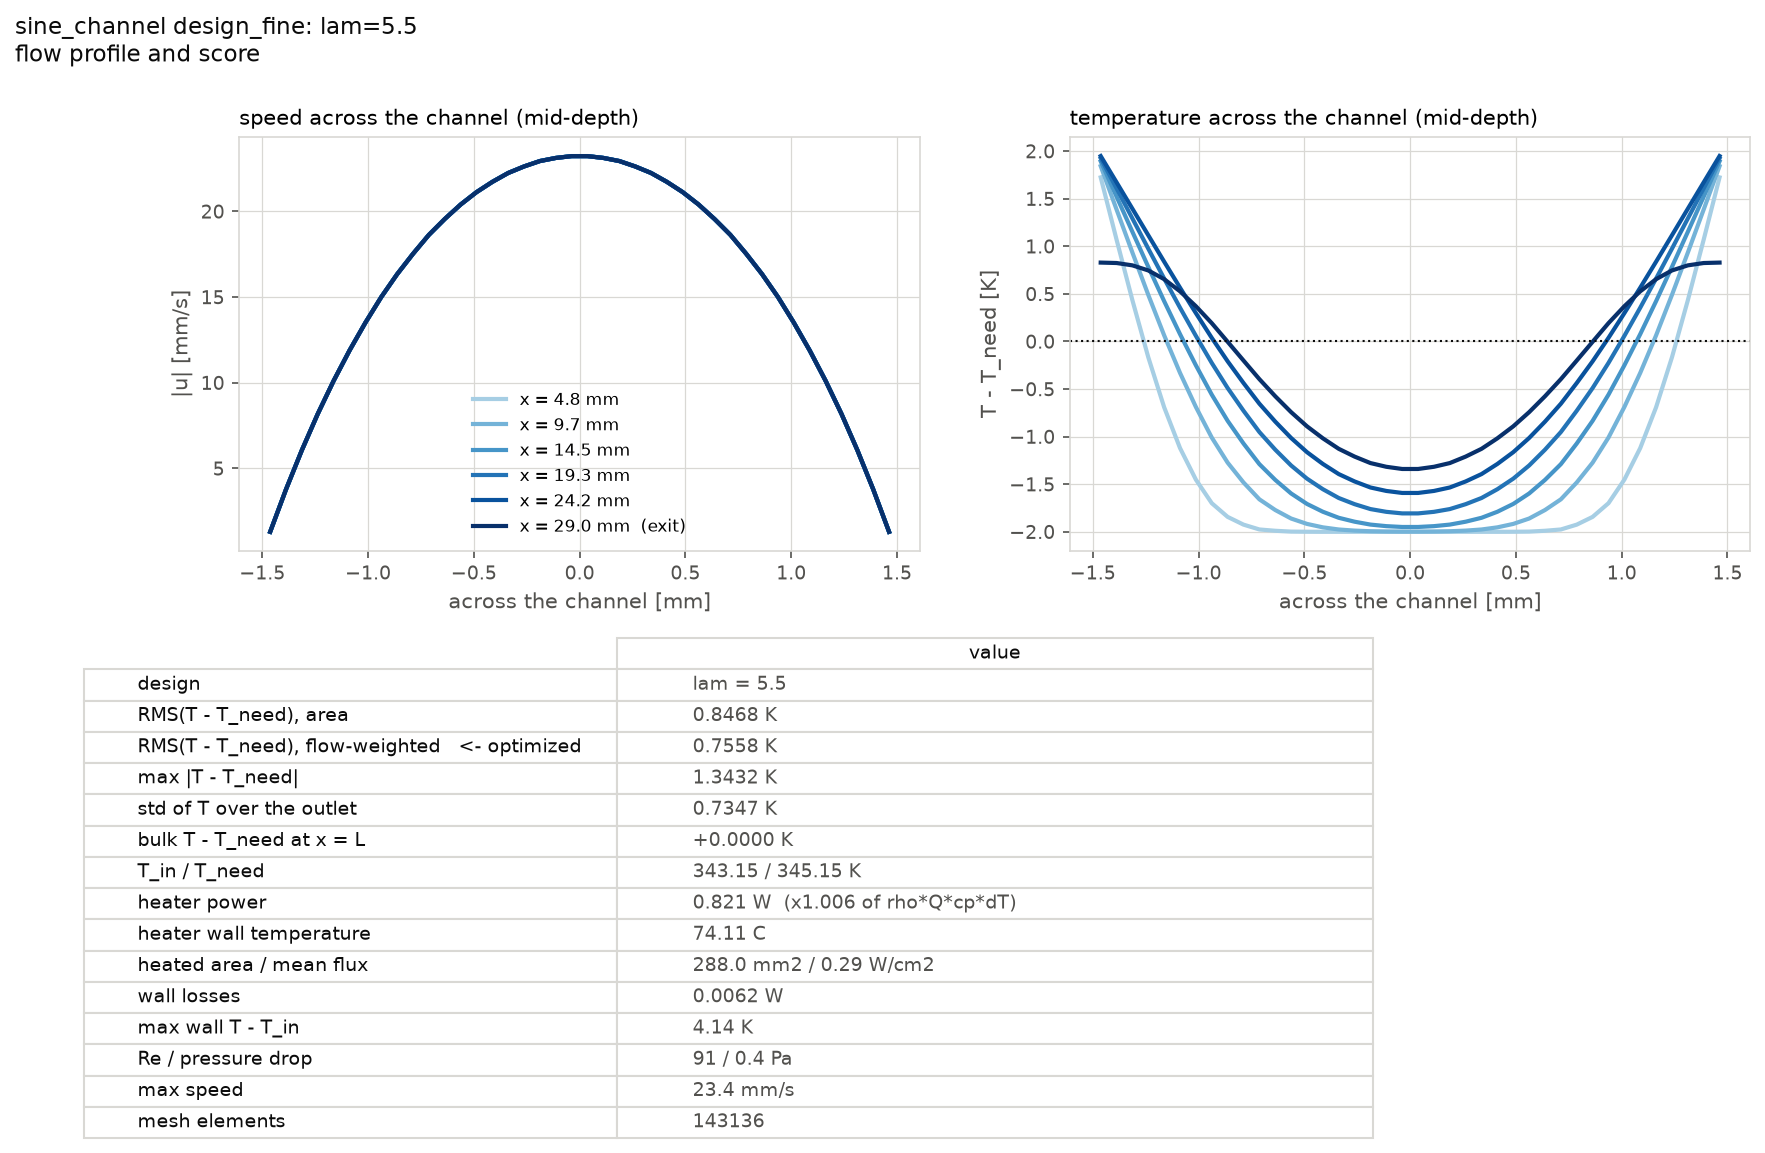
\includegraphics[width=0.8\textwidth,height=0.8\textheight,keepaspectratio]{runs/final_u3d_straight_ref_single_profile.png}
\caption{Speed and temperature across the channel at several $x$ stations, and the full score table of the design.}
\end{figure}
\begin{figure}[H]\centering
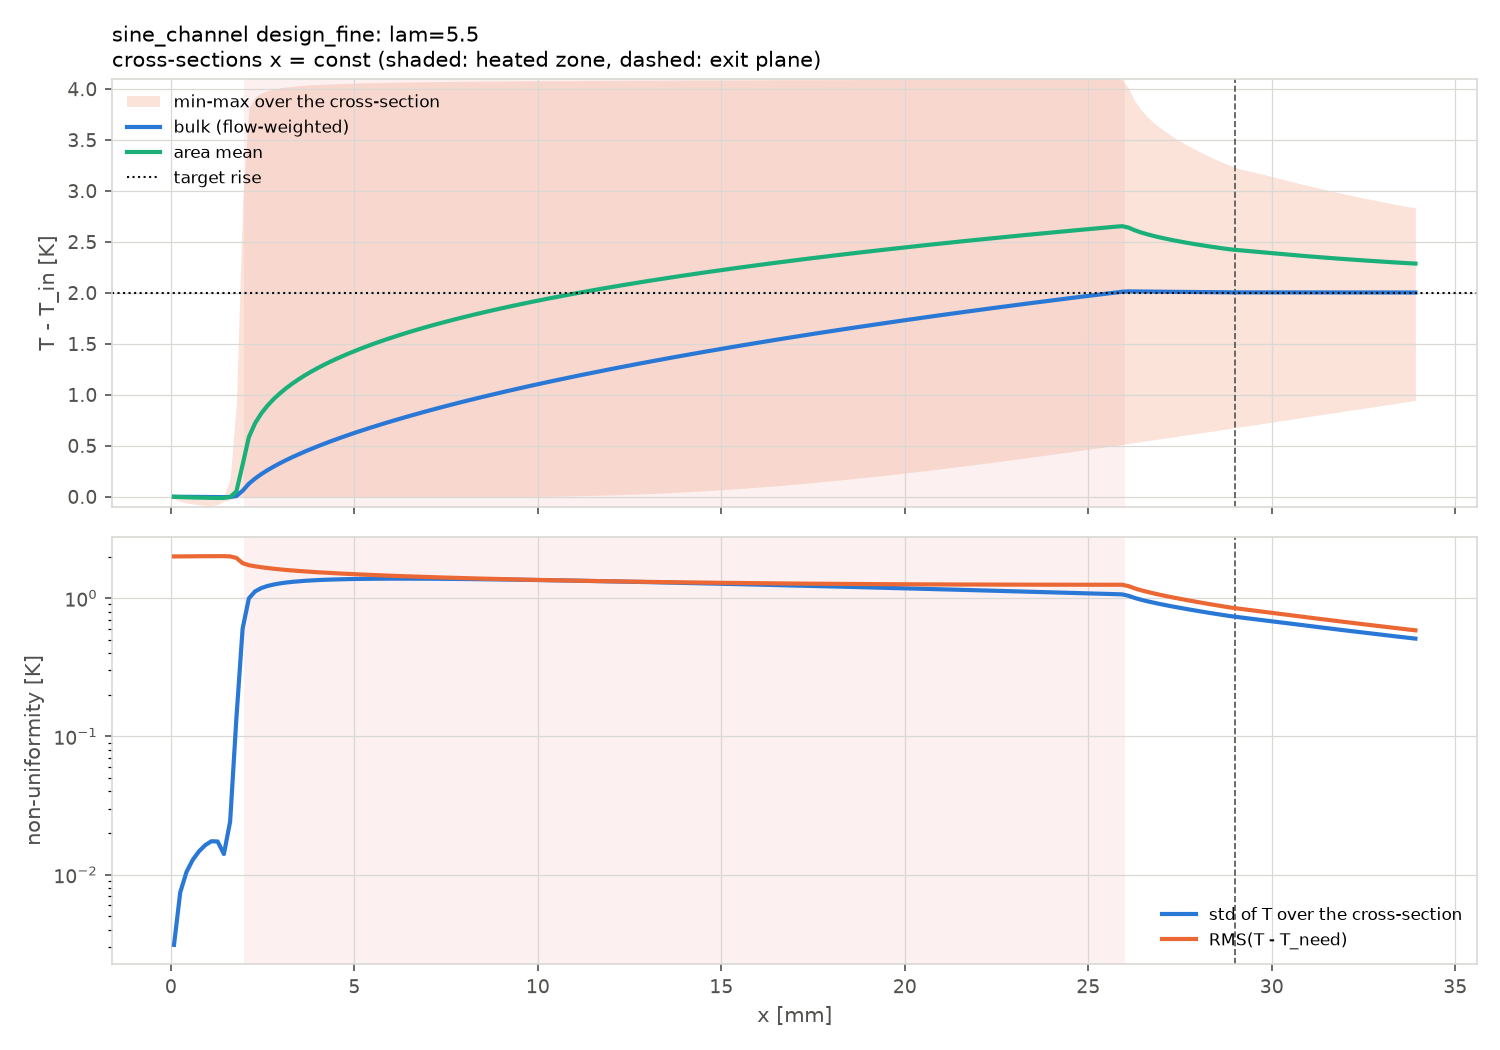
\includegraphics[width=0.8\textwidth,height=0.8\textheight,keepaspectratio]{runs/final_u3d_straight_ref_single_along_x.png}
\caption{Bulk, mean, min and max temperature along the channel.}
\end{figure}
\clearpage
\subsubsection*{3D straight reference, best heater window (1.2\mm{} at the start): 378\mK}
\noindent\texttt{runs/final\_u3d\_straight\_ref}\par\medskip
\begin{figure}[H]\centering
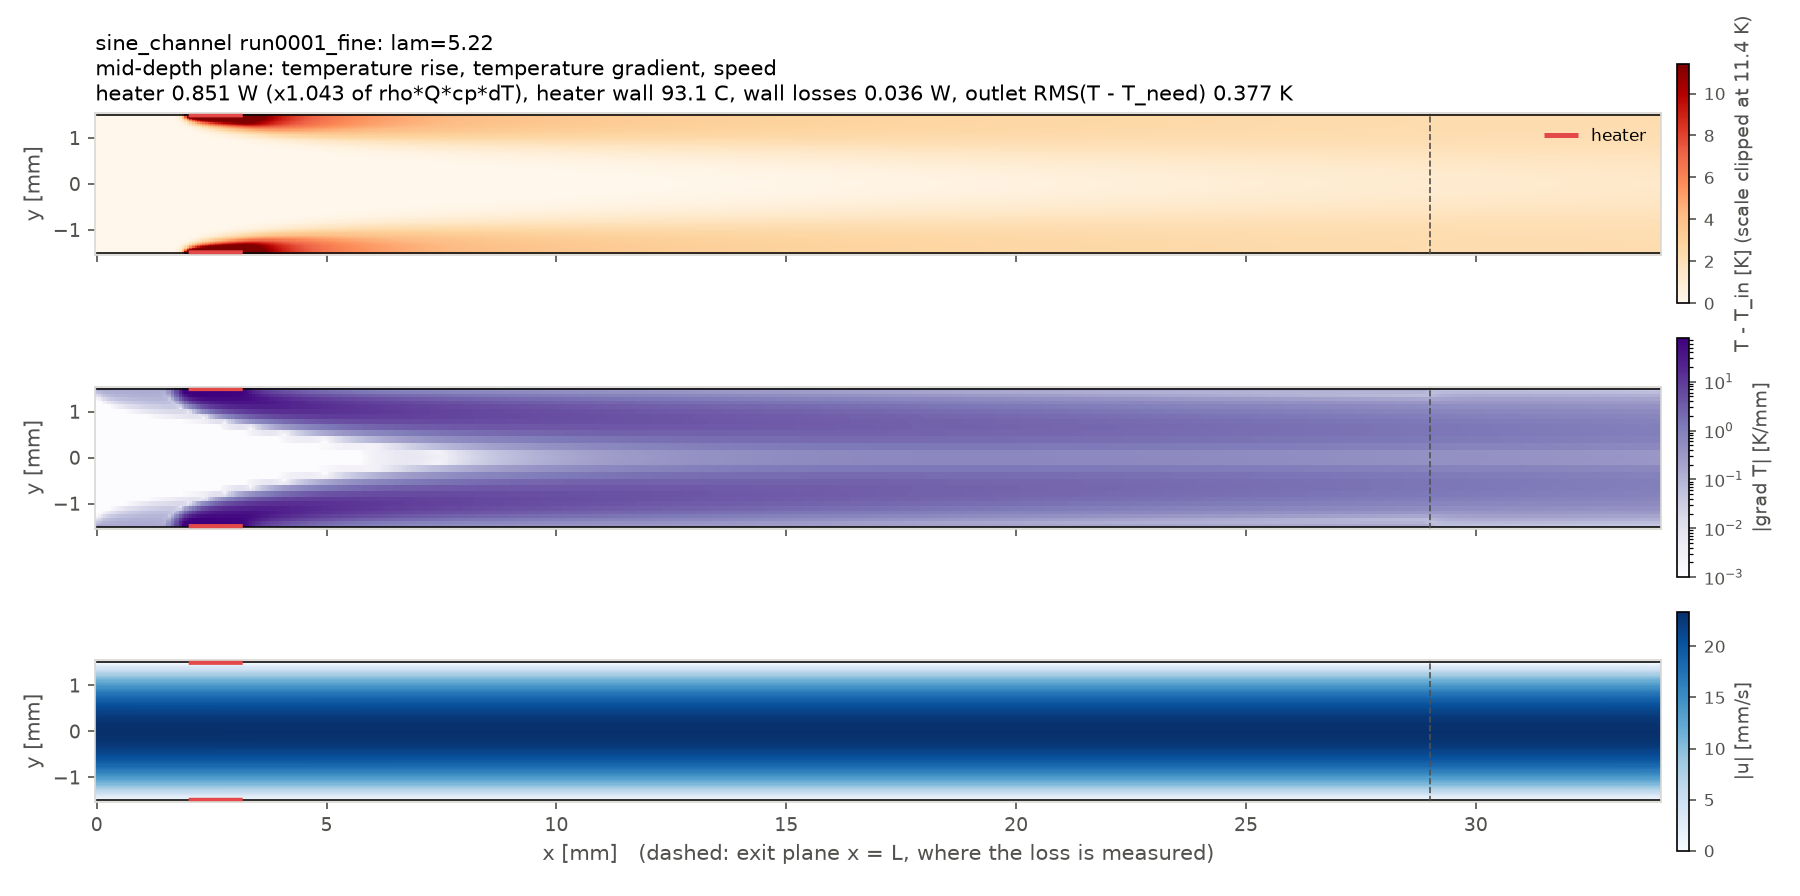
\includegraphics[width=0.95\textwidth,height=0.8\textheight,keepaspectratio]{runs/final_u3d_straight_ref_maps.png}
\caption{Temperature rise, temperature gradient and speed (mid-depth plane in 3D). Red: heated wall. The title's ``outlet RMS'' is the area-weighted $\ell_{2,\mathrm{area}}$.}
\end{figure}
\begin{figure}[H]\centering
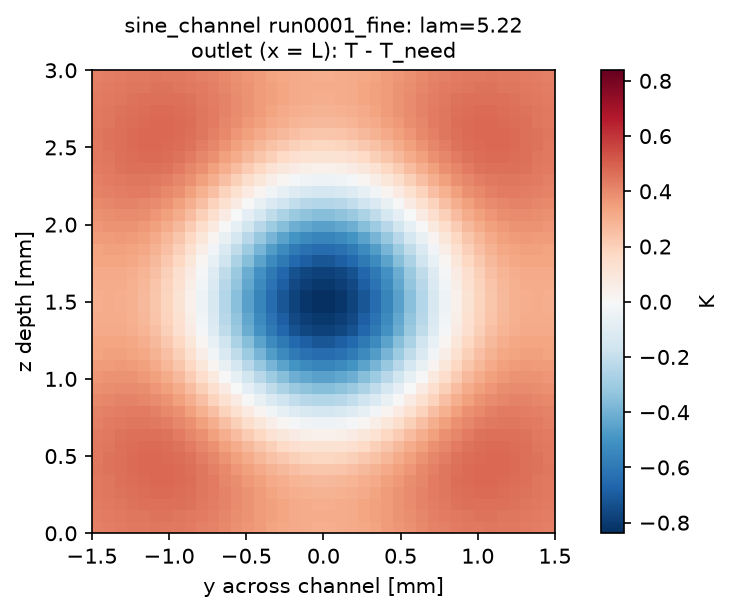
\includegraphics[width=0.75\textwidth,height=0.8\textheight,keepaspectratio]{runs/final_u3d_straight_ref_outlet.png}
\caption{Outlet temperature (and, in 3D, the outlet plane).}
\end{figure}
\begin{figure}[H]\centering
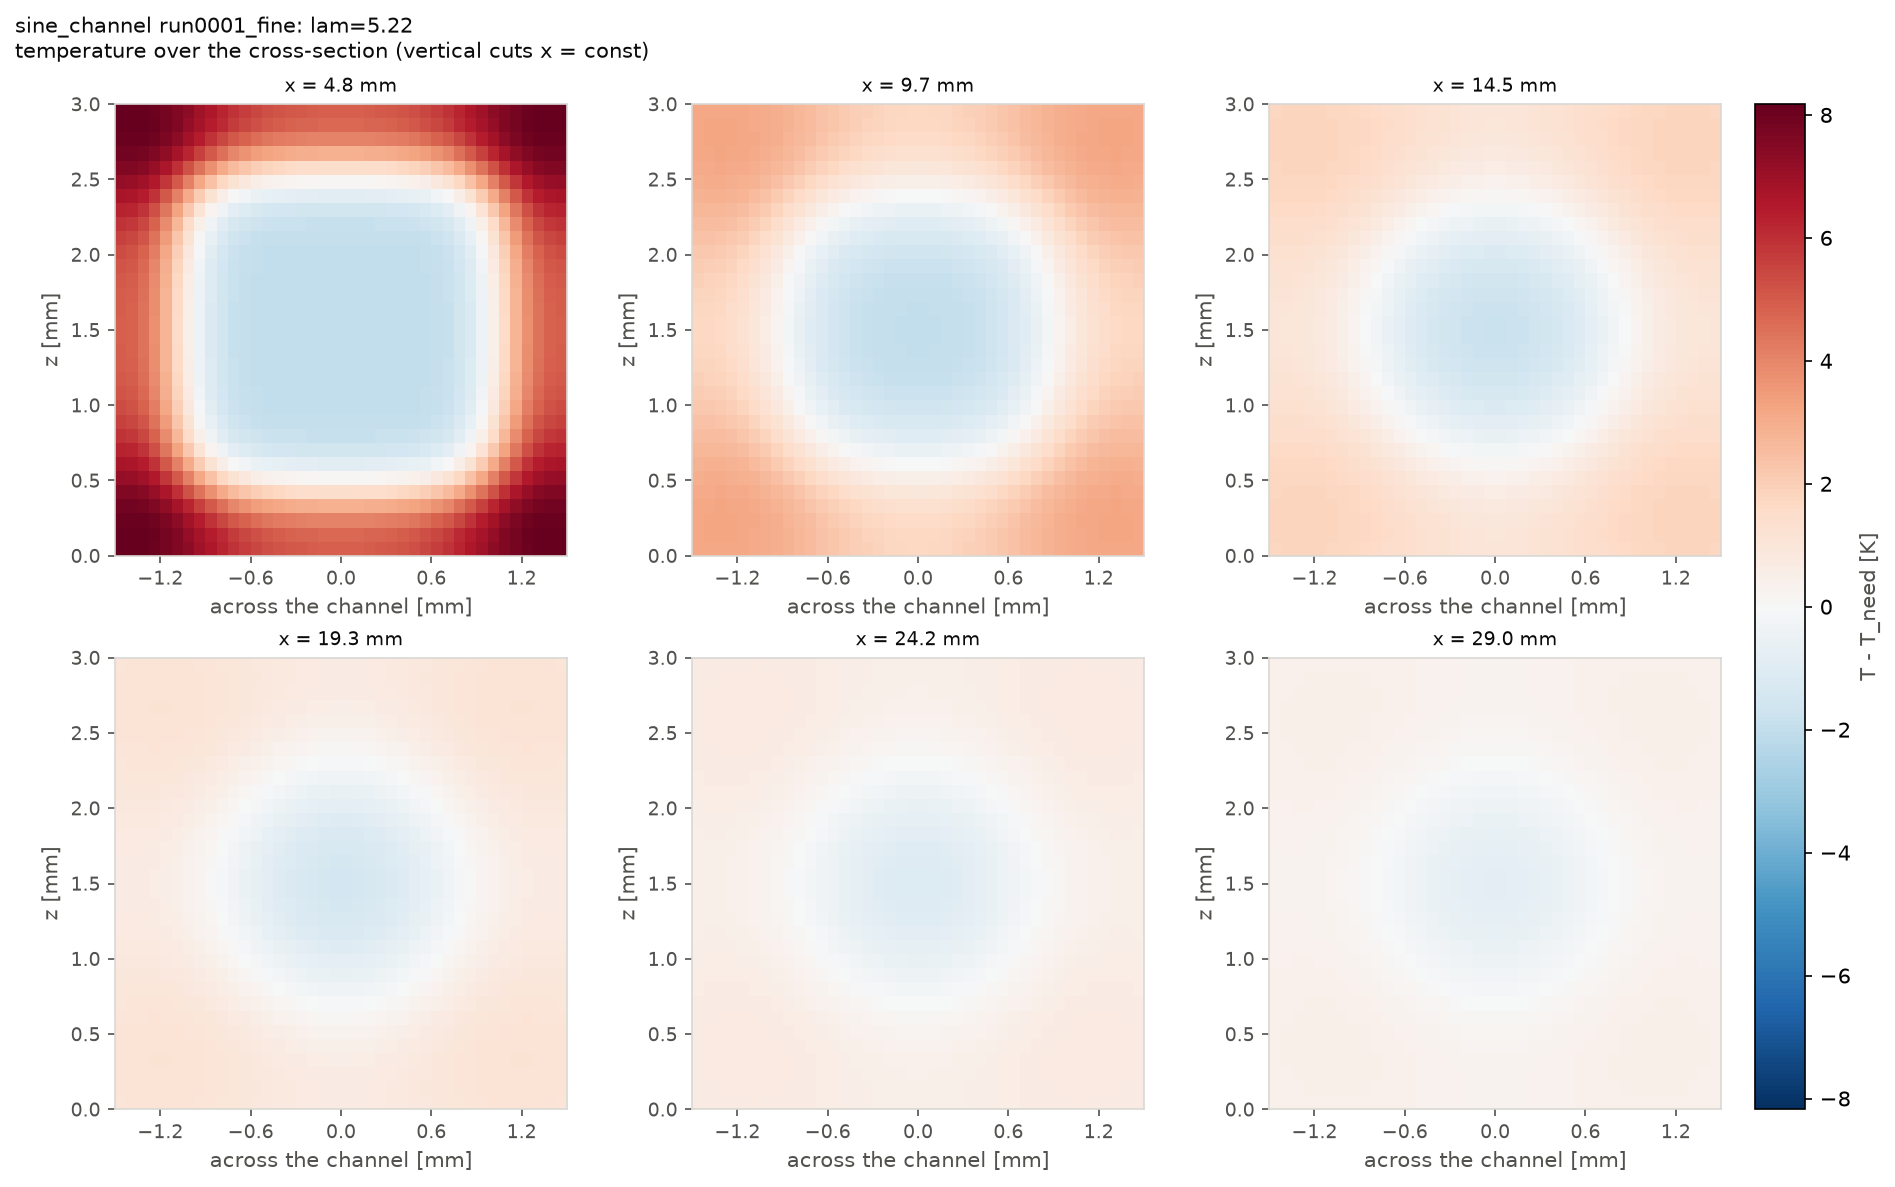
\includegraphics[width=0.62\textwidth,height=0.8\textheight,keepaspectratio]{runs/final_u3d_straight_ref_slices.png}
\caption{Temperature profiles across the channel at several $x$ stations.}
\end{figure}
\begin{figure}[H]\centering
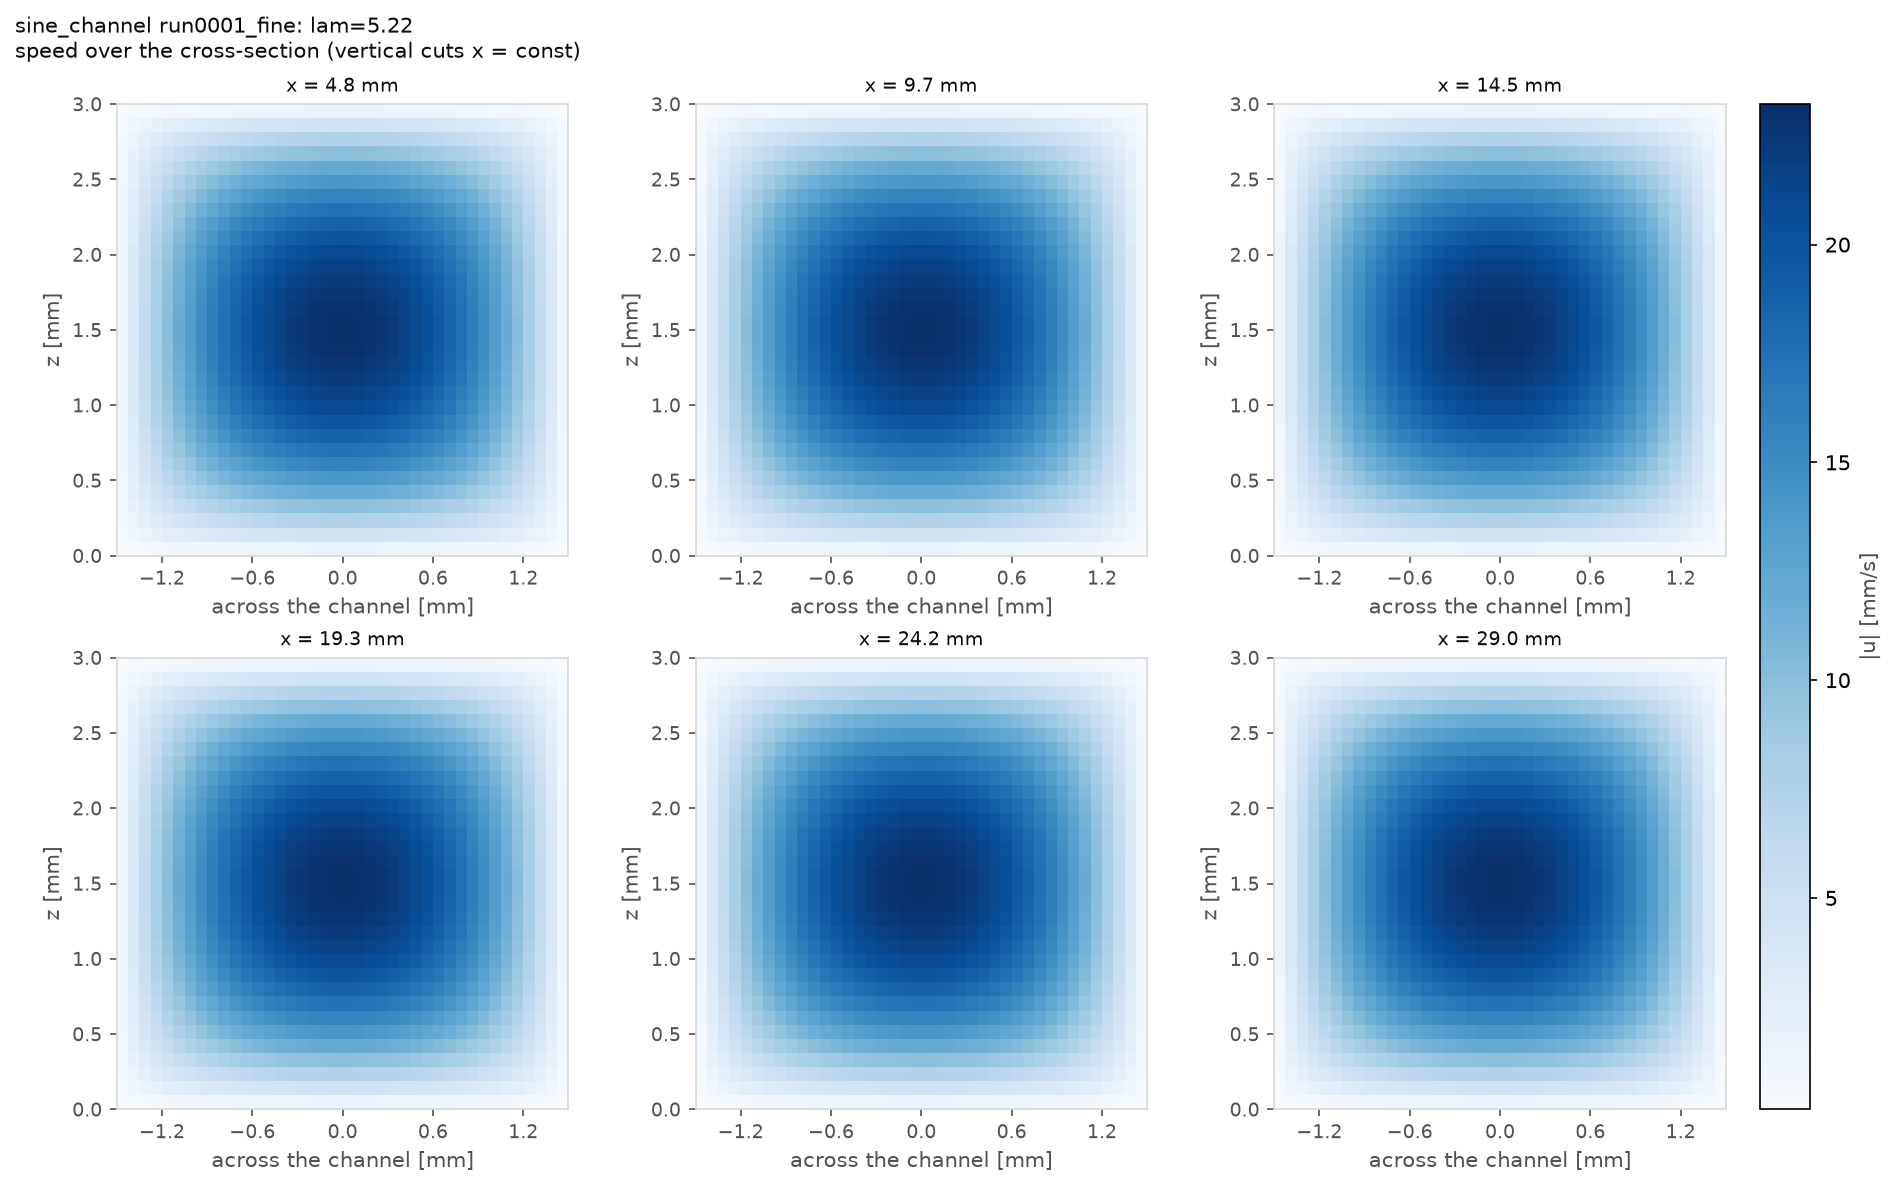
\includegraphics[width=0.85\textwidth,height=0.8\textheight,keepaspectratio]{runs/final_u3d_straight_ref_slices_u.png}
\caption{Velocity on cross-sections (3D).}
\end{figure}
\begin{figure}[H]\centering
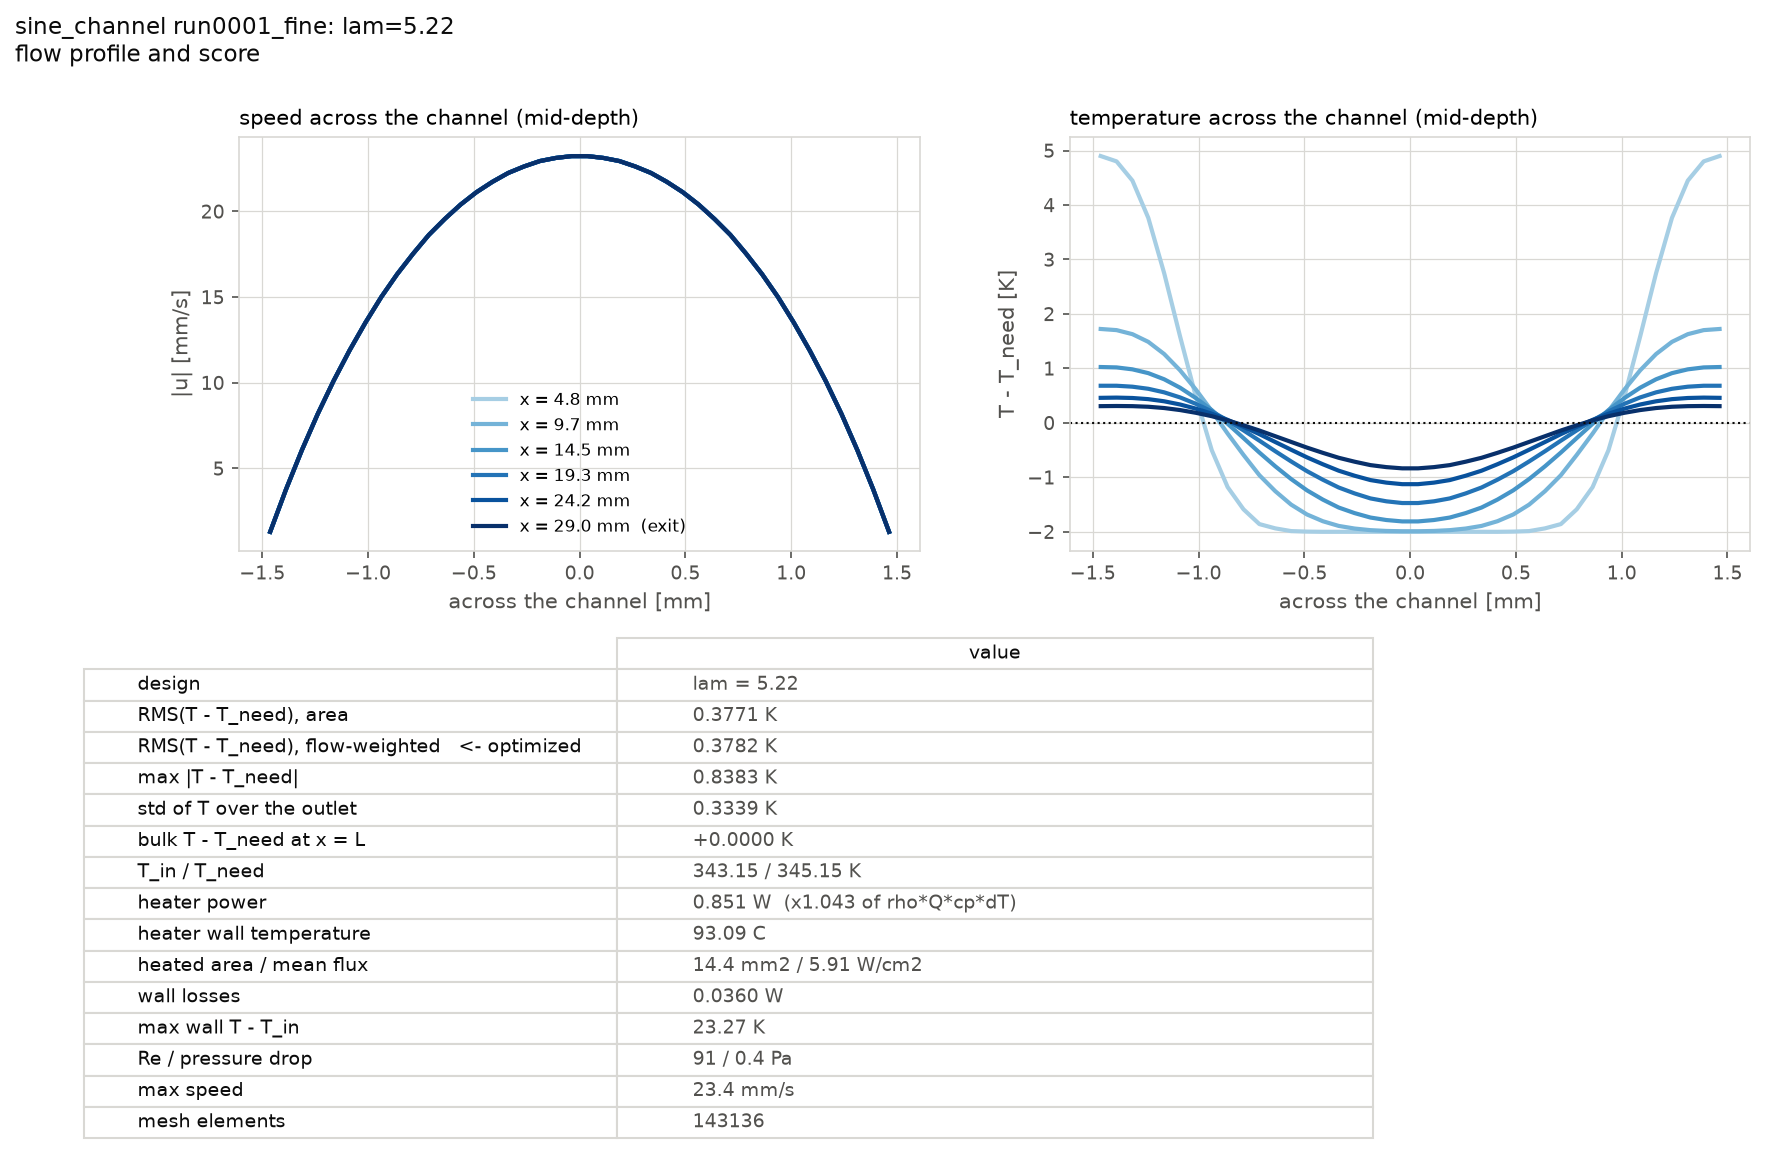
\includegraphics[width=0.8\textwidth,height=0.8\textheight,keepaspectratio]{runs/final_u3d_straight_ref_profile.png}
\caption{Speed and temperature across the channel at several $x$ stations, and the full score table of the design.}
\end{figure}
\begin{figure}[H]\centering
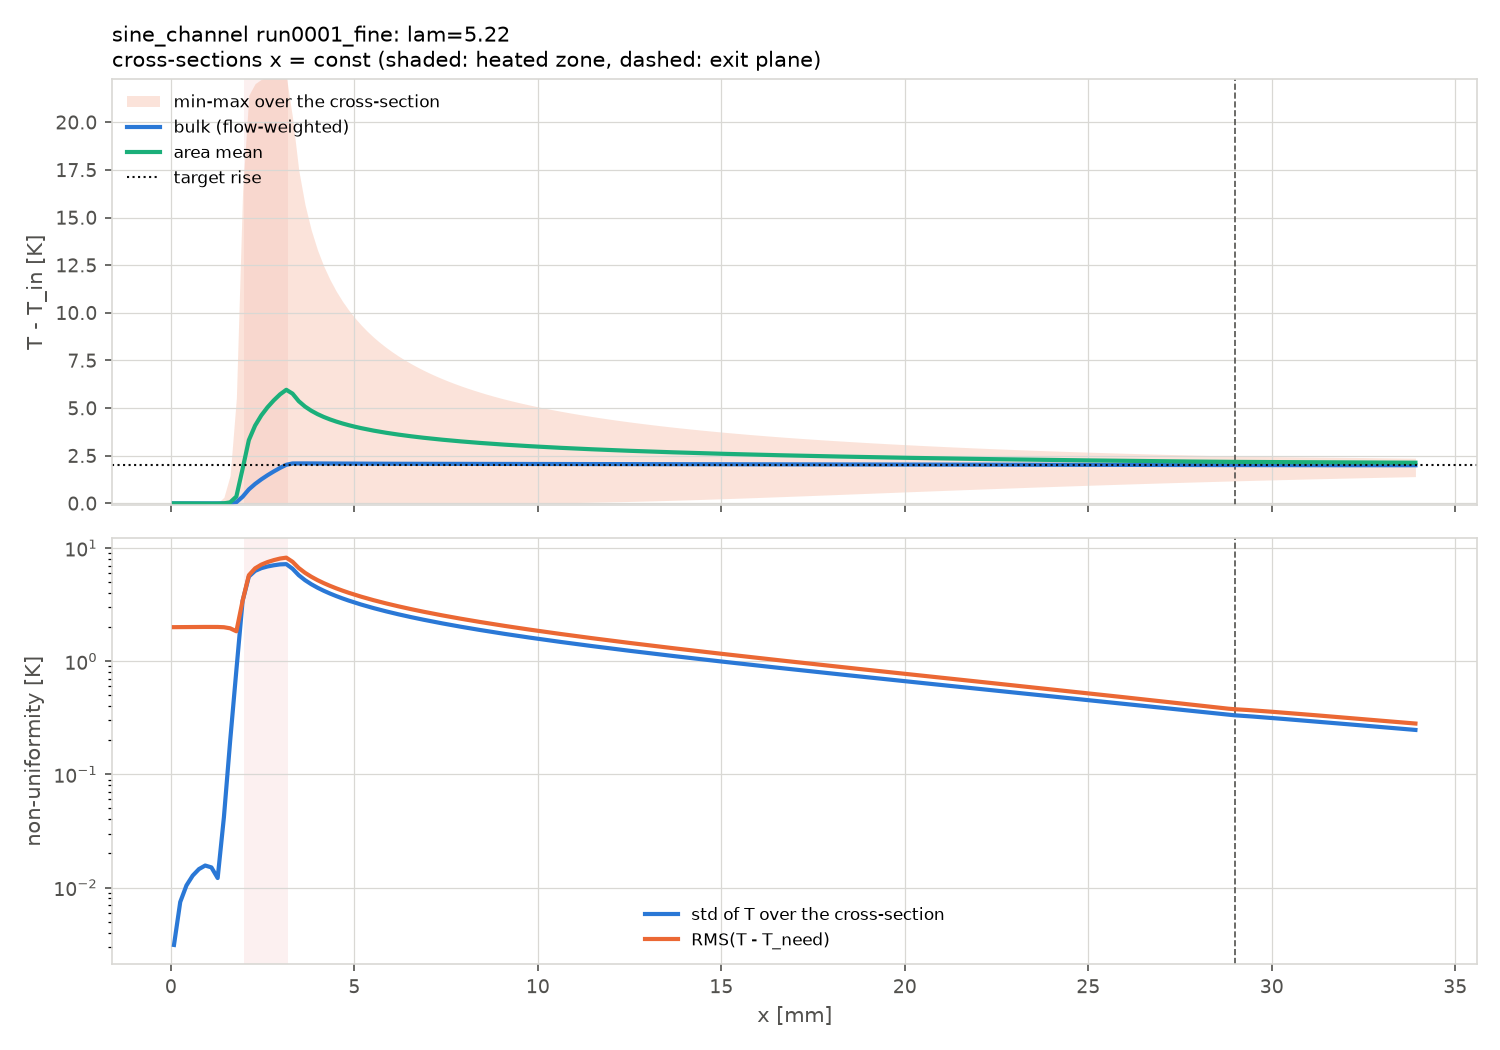
\includegraphics[width=0.8\textwidth,height=0.8\textheight,keepaspectratio]{runs/final_u3d_straight_ref_along_x.png}
\caption{Bulk, mean, min and max temperature along the channel.}
\end{figure}
\clearpage
\subsubsection*{3D serpentine, BO best \#29 ($\lambda$ 7.26, $A$ 3.5, heater 19.2\mm): 27.4\mK}
\noindent\texttt{runs/final\_u3d\_serp}\par\medskip
\begin{figure}[H]\centering
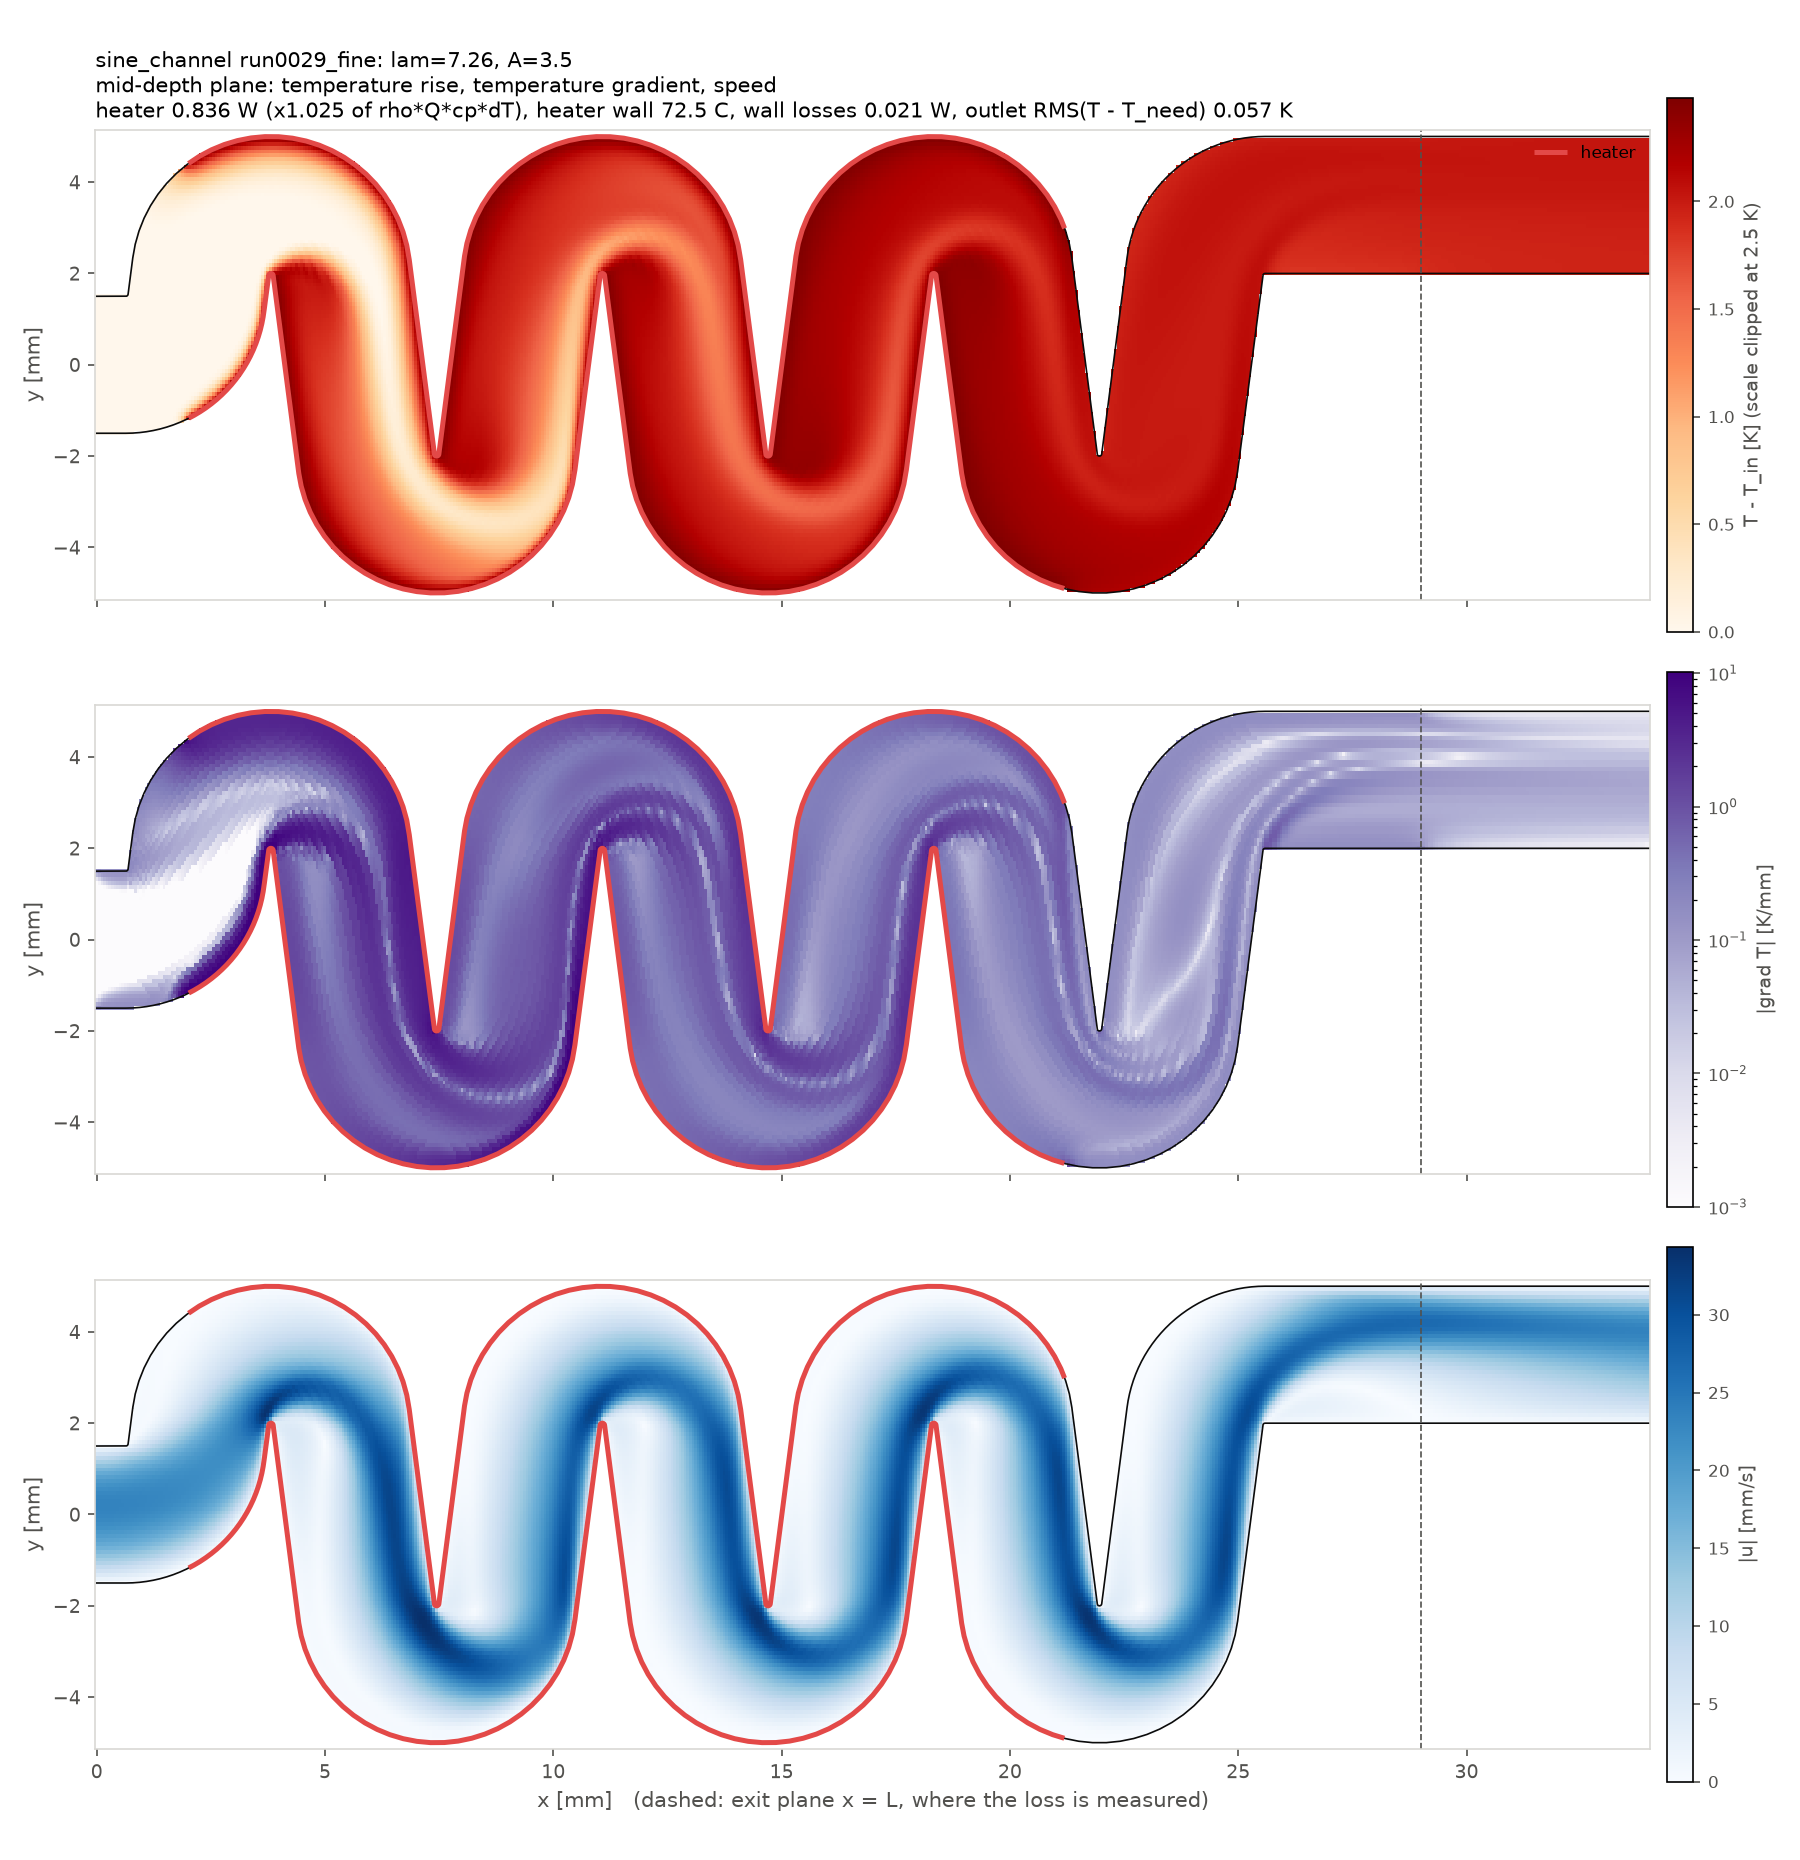
\includegraphics[width=0.95\textwidth,height=0.8\textheight,keepaspectratio]{runs/final_u3d_serp_maps.png}
\caption{Temperature rise, temperature gradient and speed (mid-depth plane in 3D). Red: heated wall. The title's ``outlet RMS'' is the area-weighted $\ell_{2,\mathrm{area}}$.}
\end{figure}
\begin{figure}[H]\centering
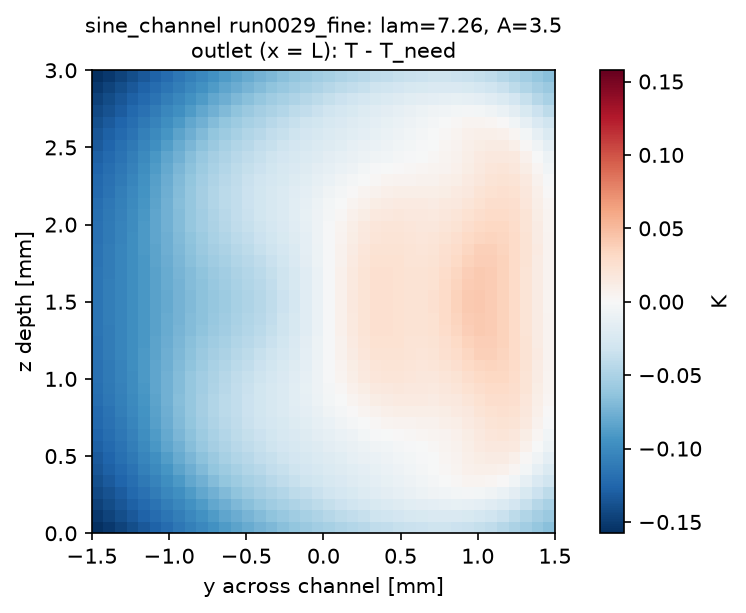
\includegraphics[width=0.75\textwidth,height=0.8\textheight,keepaspectratio]{runs/final_u3d_serp_outlet.png}
\caption{Outlet temperature (and, in 3D, the outlet plane).}
\end{figure}
\begin{figure}[H]\centering
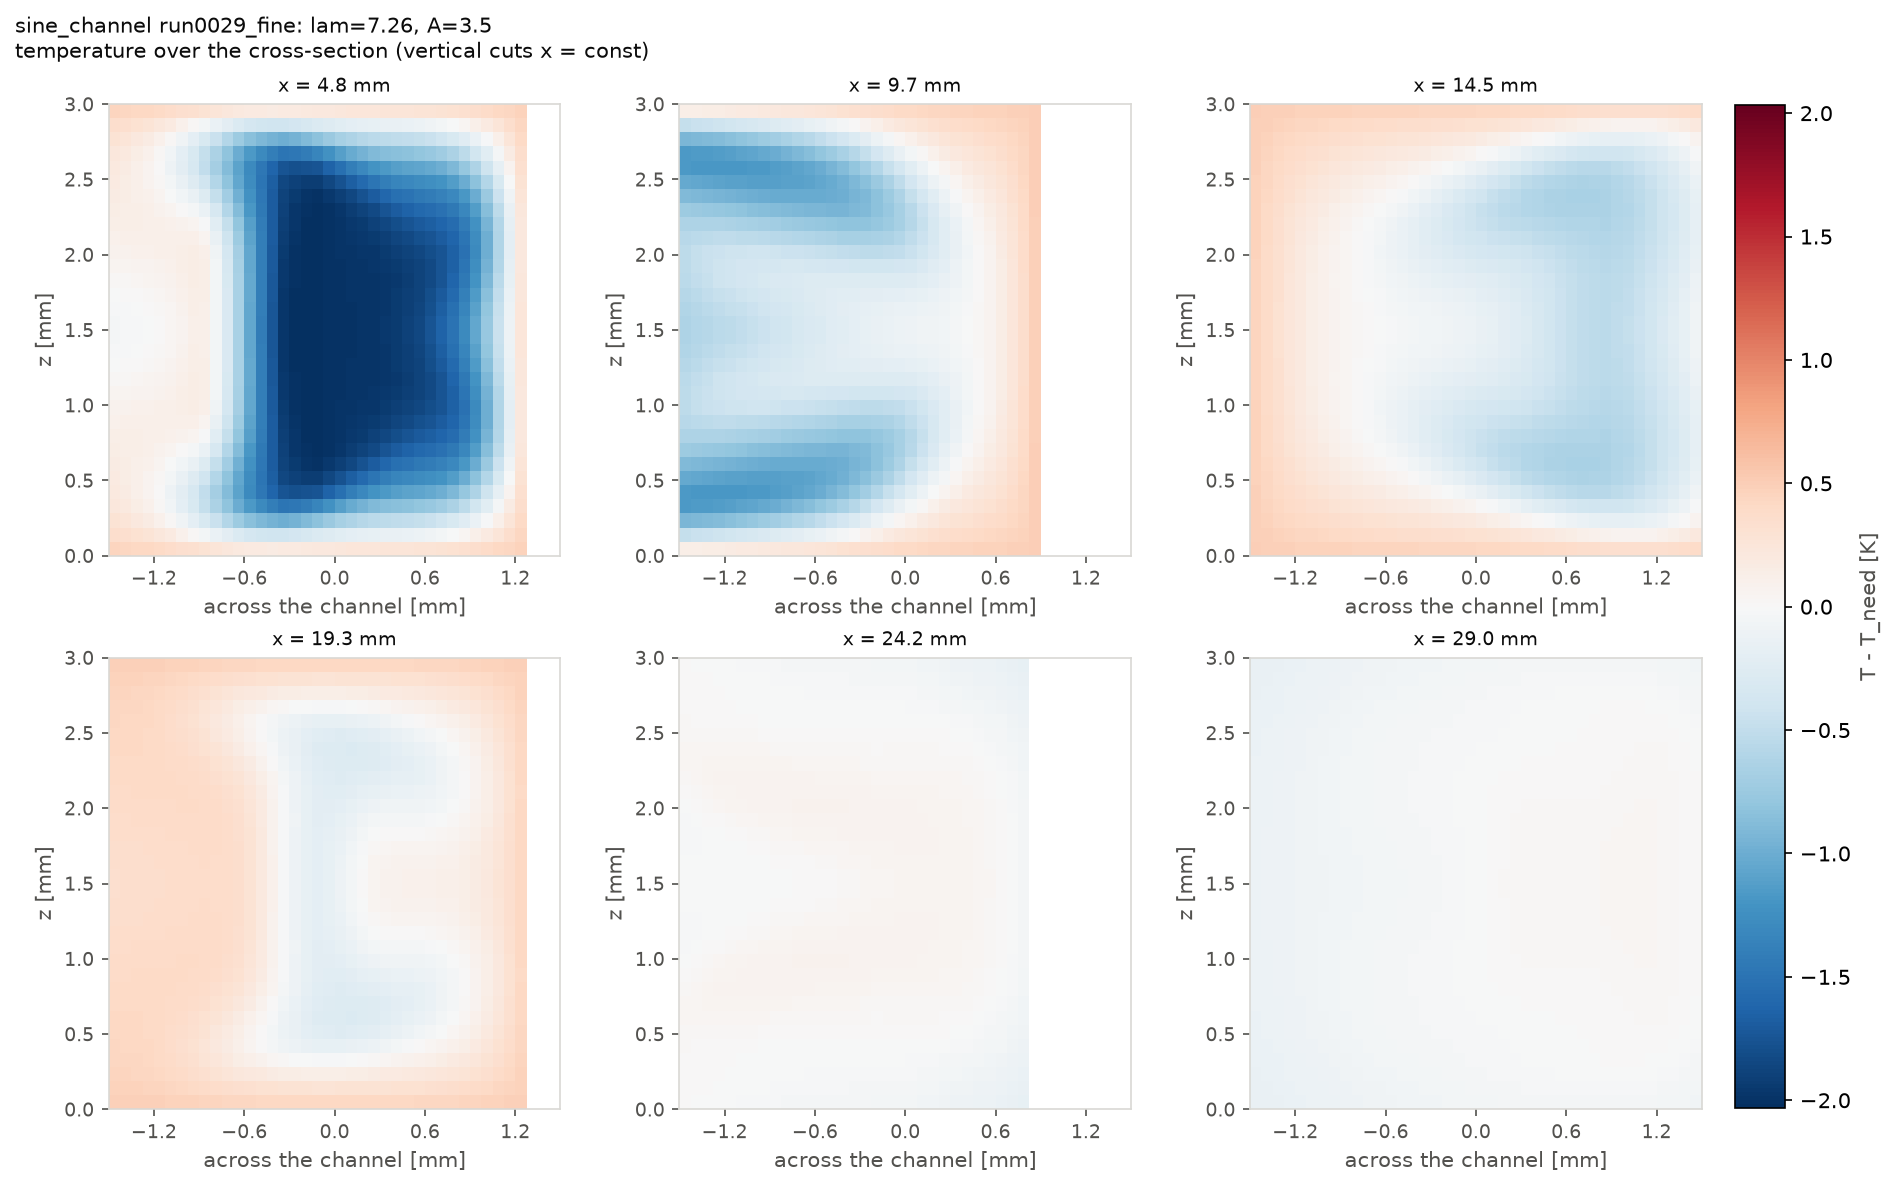
\includegraphics[width=0.62\textwidth,height=0.8\textheight,keepaspectratio]{runs/final_u3d_serp_slices.png}
\caption{Temperature profiles across the channel at several $x$ stations.}
\end{figure}
\begin{figure}[H]\centering
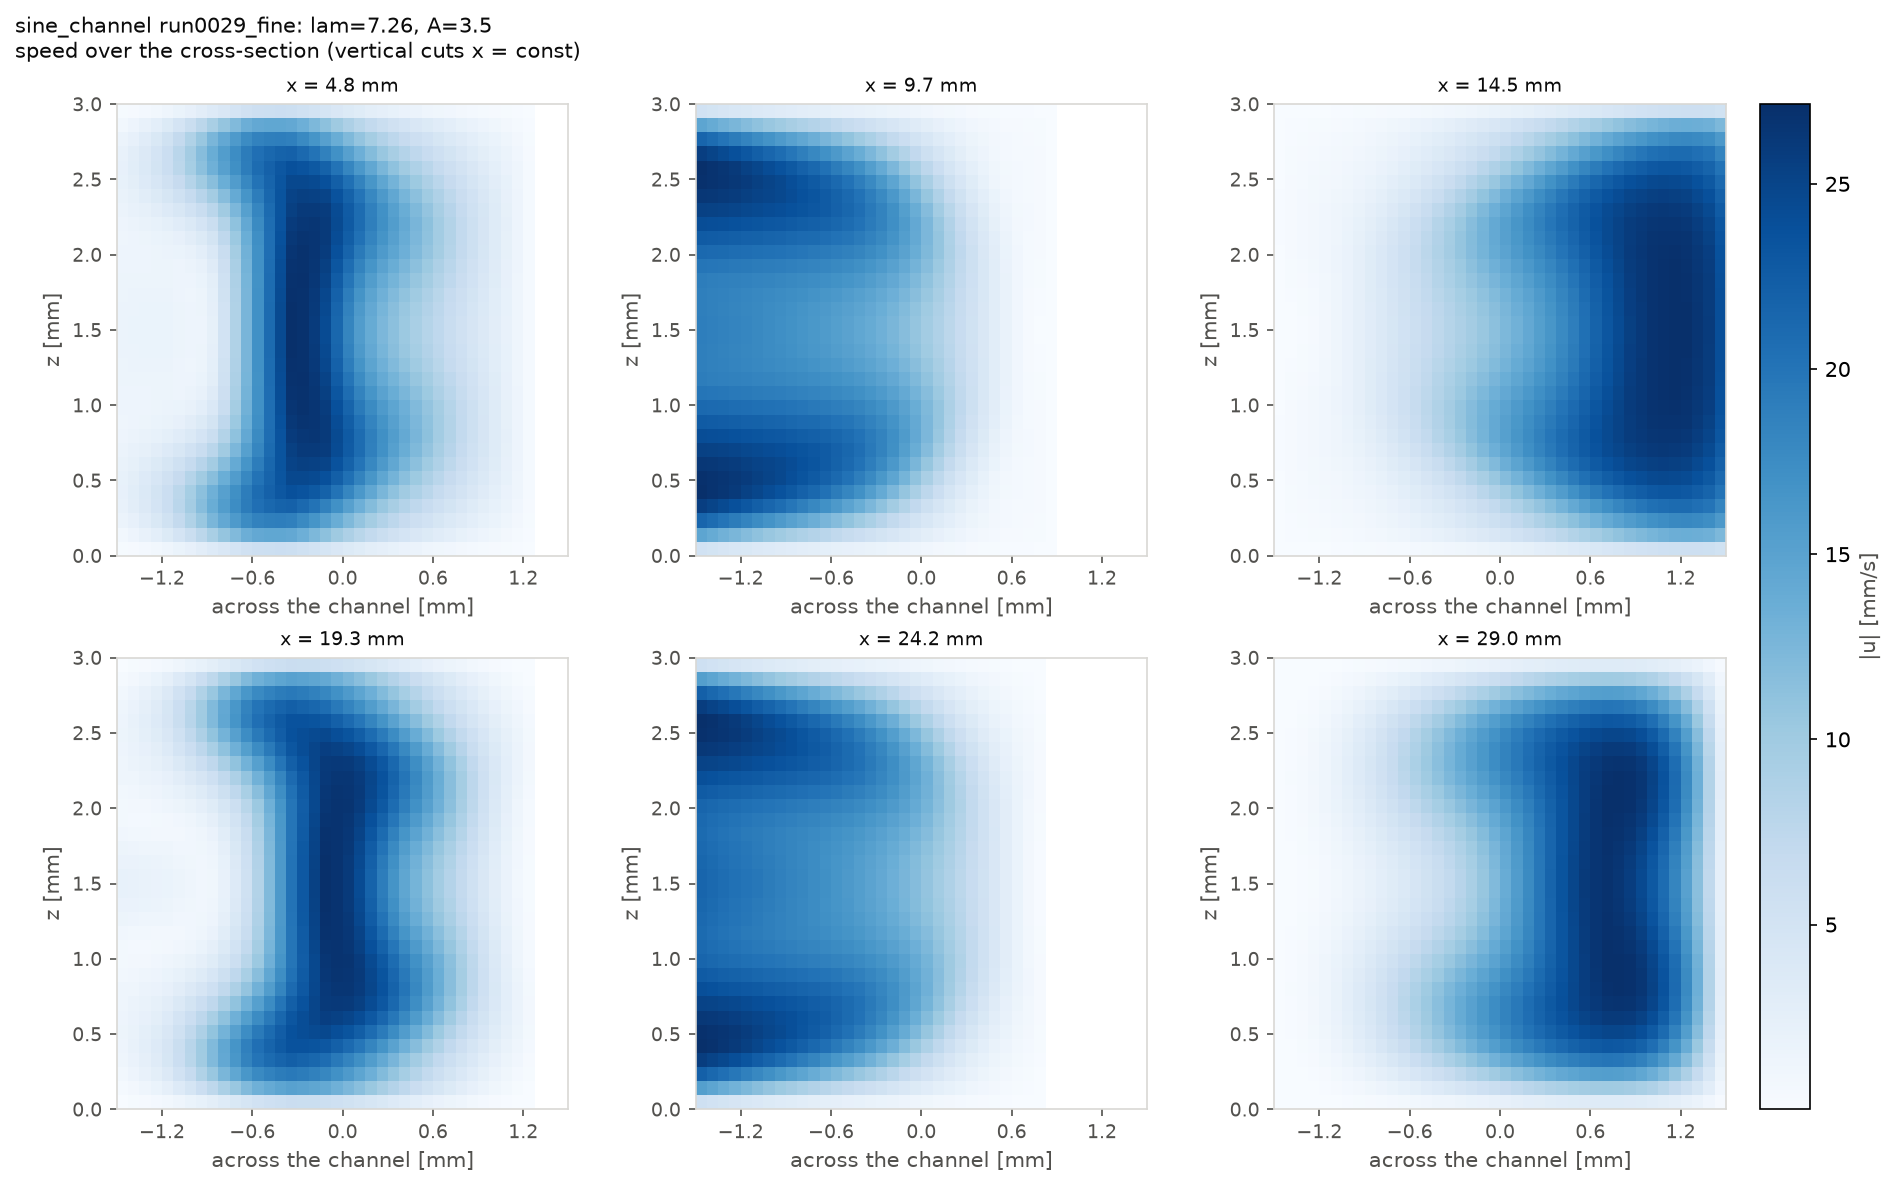
\includegraphics[width=0.85\textwidth,height=0.8\textheight,keepaspectratio]{runs/final_u3d_serp_slices_u.png}
\caption{Velocity on cross-sections (3D).}
\end{figure}
\begin{figure}[H]\centering
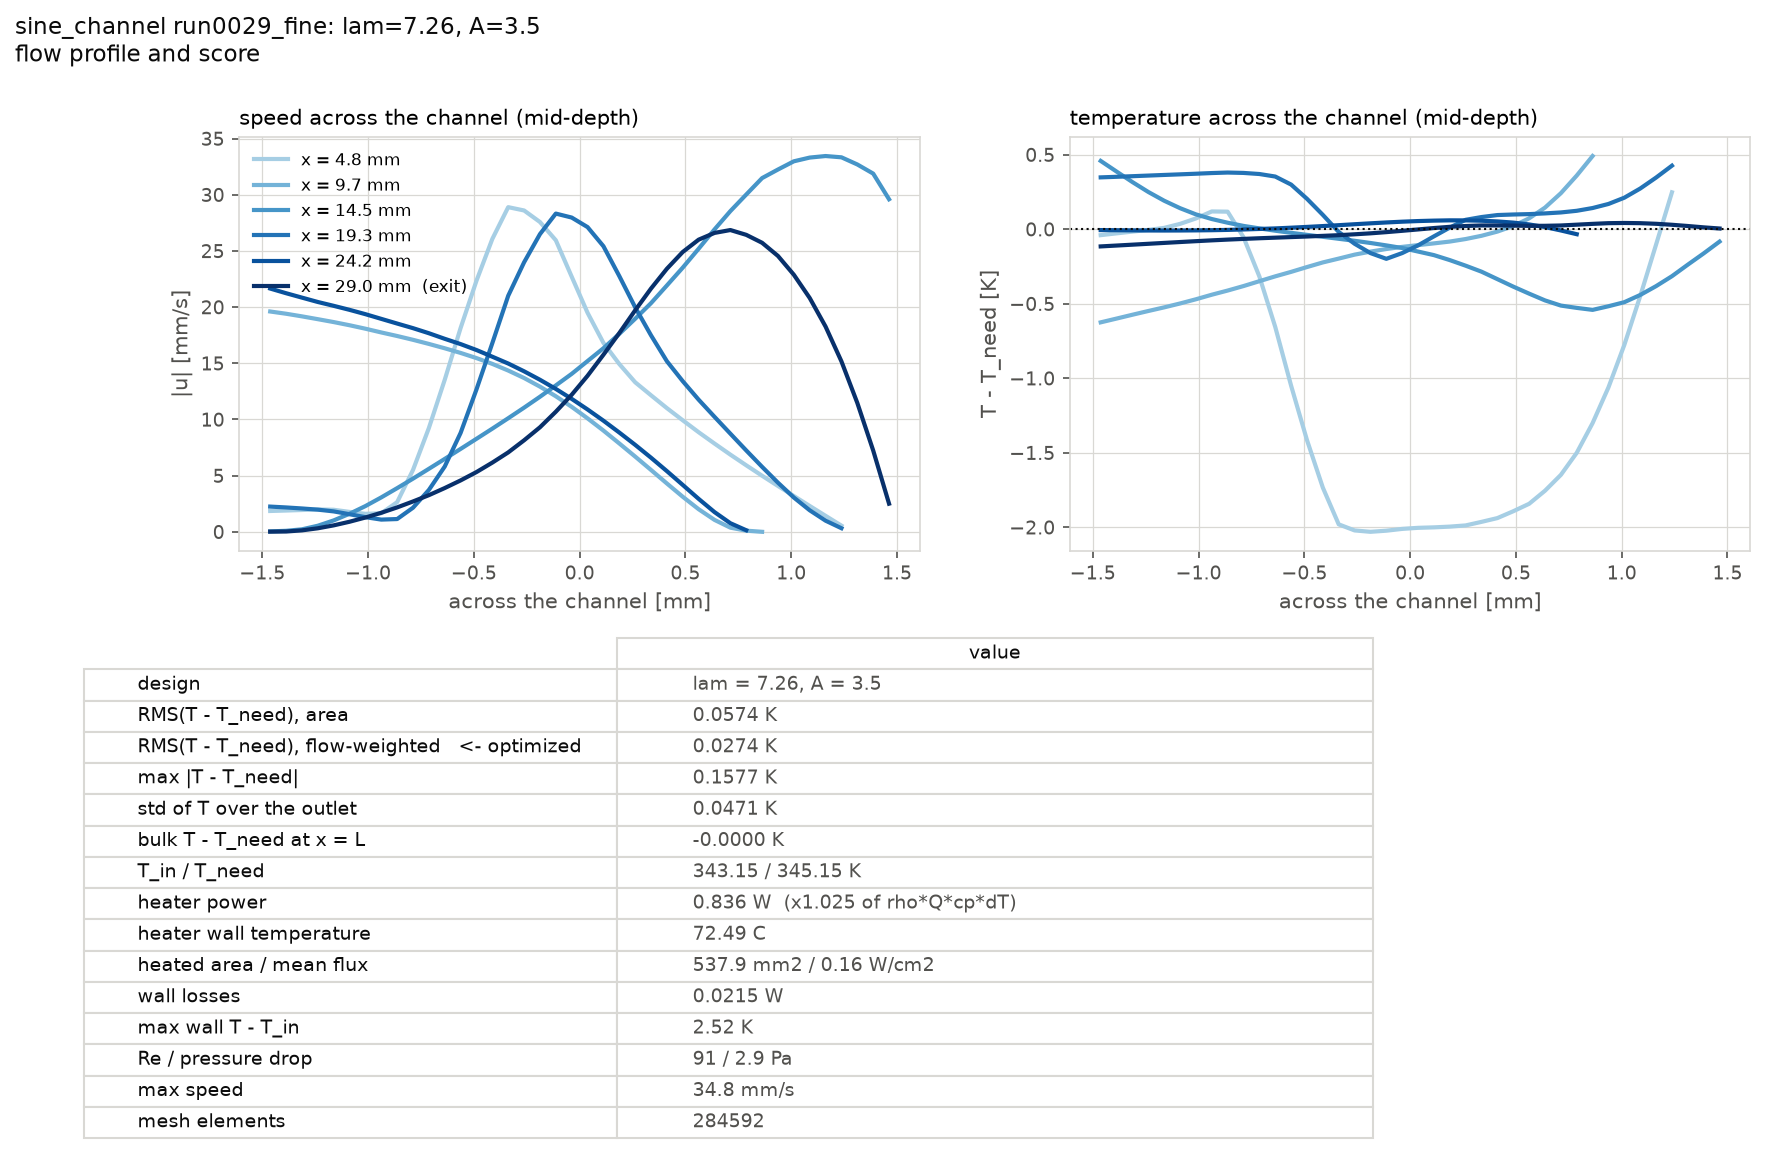
\includegraphics[width=0.8\textwidth,height=0.8\textheight,keepaspectratio]{runs/final_u3d_serp_profile.png}
\caption{Speed and temperature across the channel at several $x$ stations, and the full score table of the design.}
\end{figure}
\begin{figure}[H]\centering
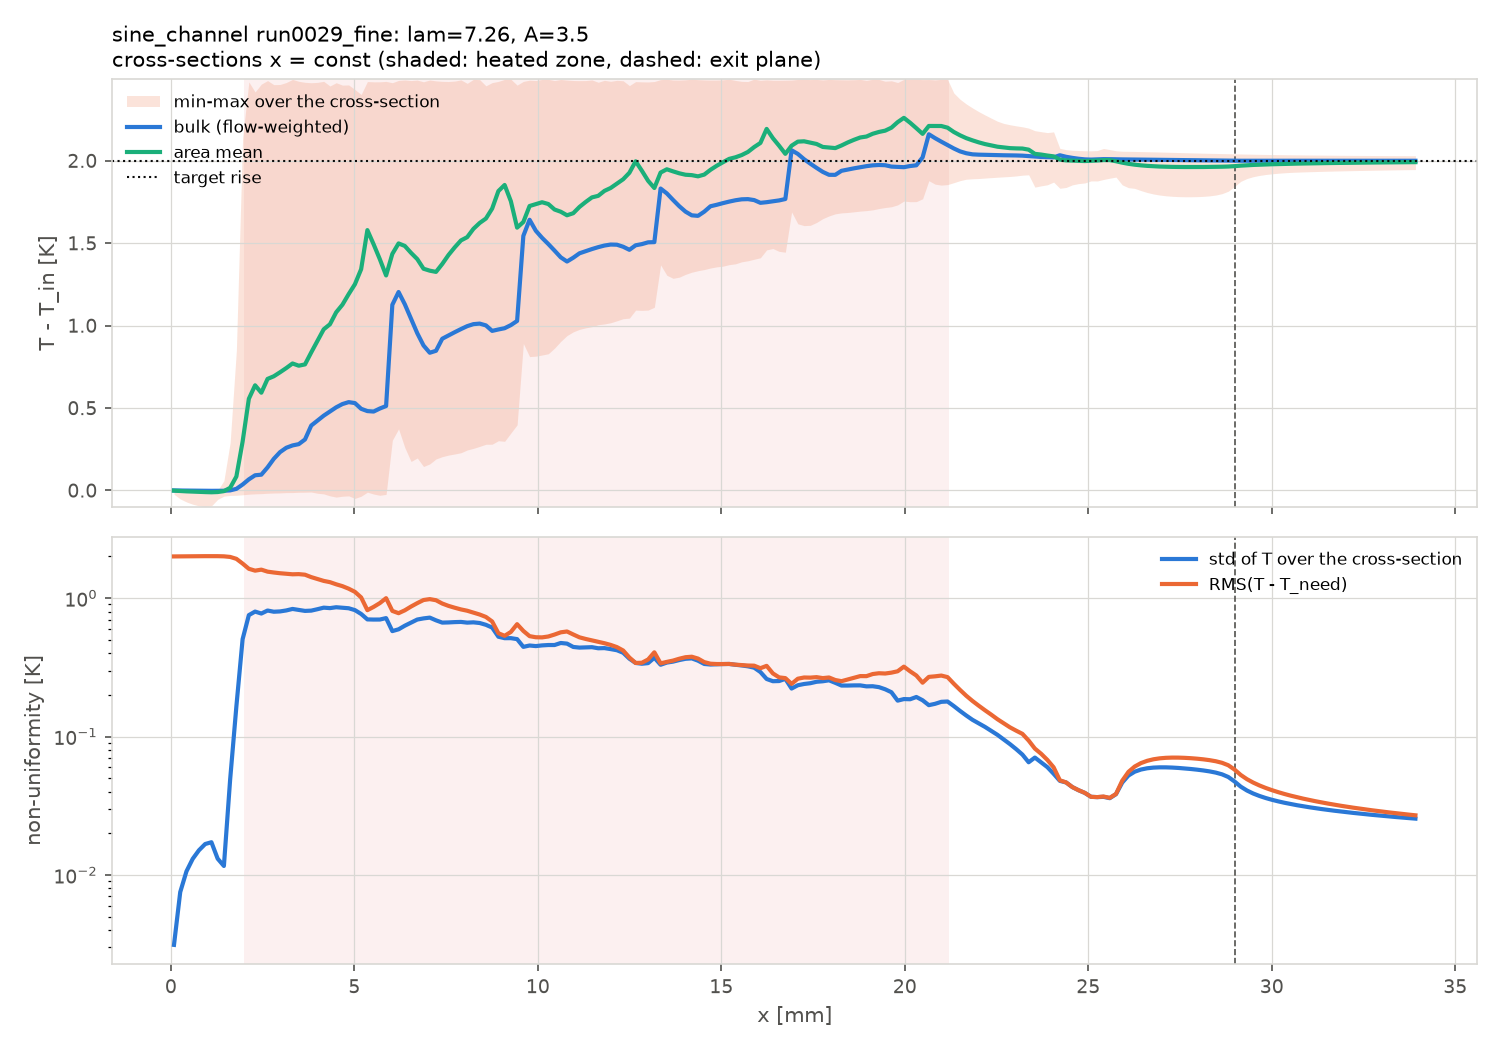
\includegraphics[width=0.8\textwidth,height=0.8\textheight,keepaspectratio]{runs/final_u3d_serp_along_x.png}
\caption{Bulk, mean, min and max temperature along the channel.}
\end{figure}
\begin{figure}[H]\centering
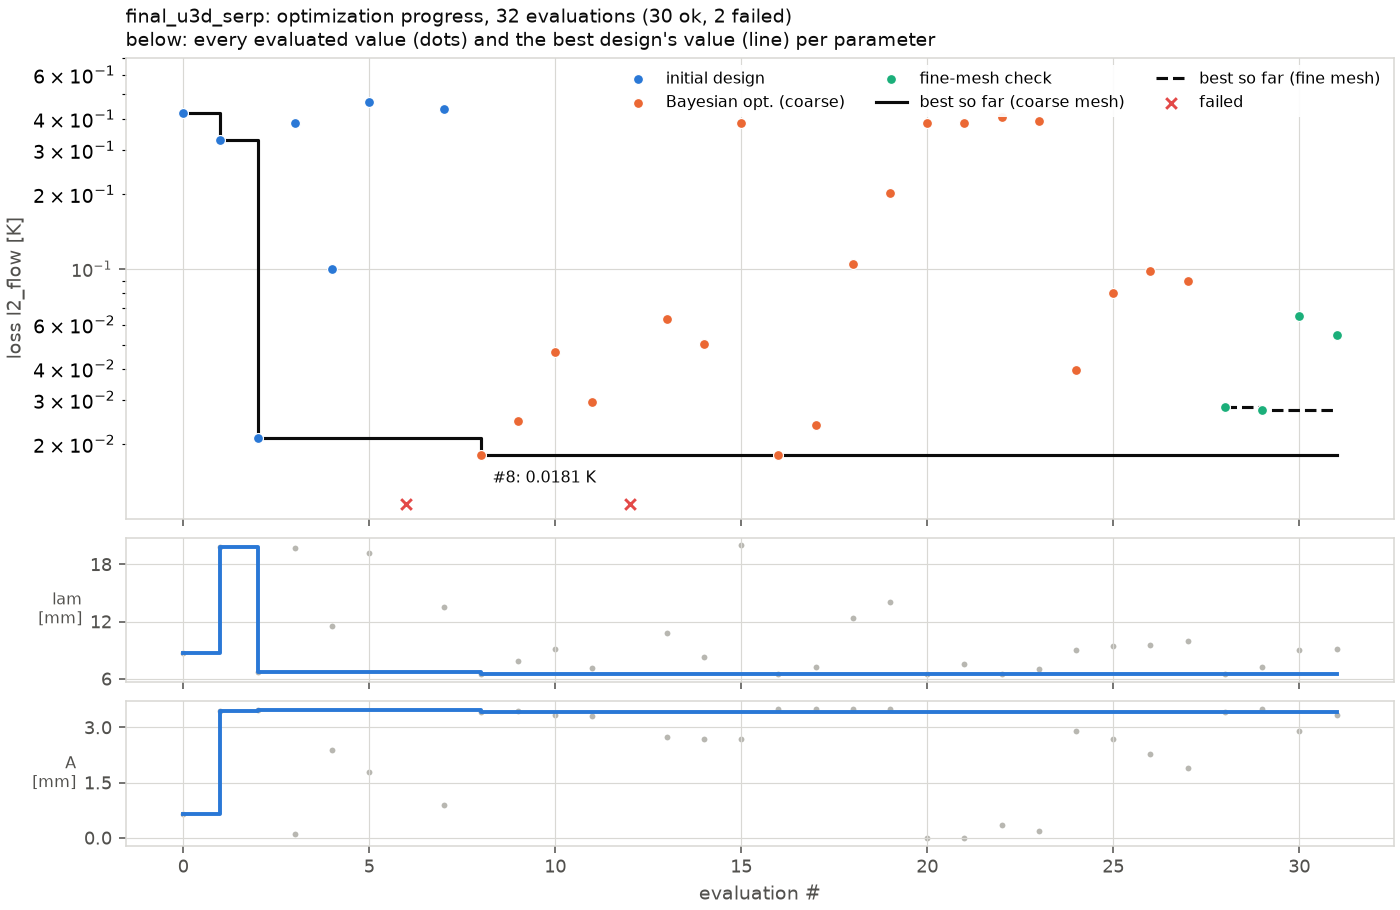
\includegraphics[width=0.85\textwidth]{runs/final_u3d_serp_progress_loss.png}
\caption{Search history: loss of every evaluation, best so far, and the parameters.}
\end{figure}
\subsection{Four branches, 2D}
\clearpage
\subsubsection*{Branched straight reference, analytic openings $\rho$ 0.532, fully heated: spread 970\mK, flow 0.87\,\%}
\noindent\texttt{runs/final\_b2d\_straight\_ref}\par\medskip
\begin{figure}[H]\centering
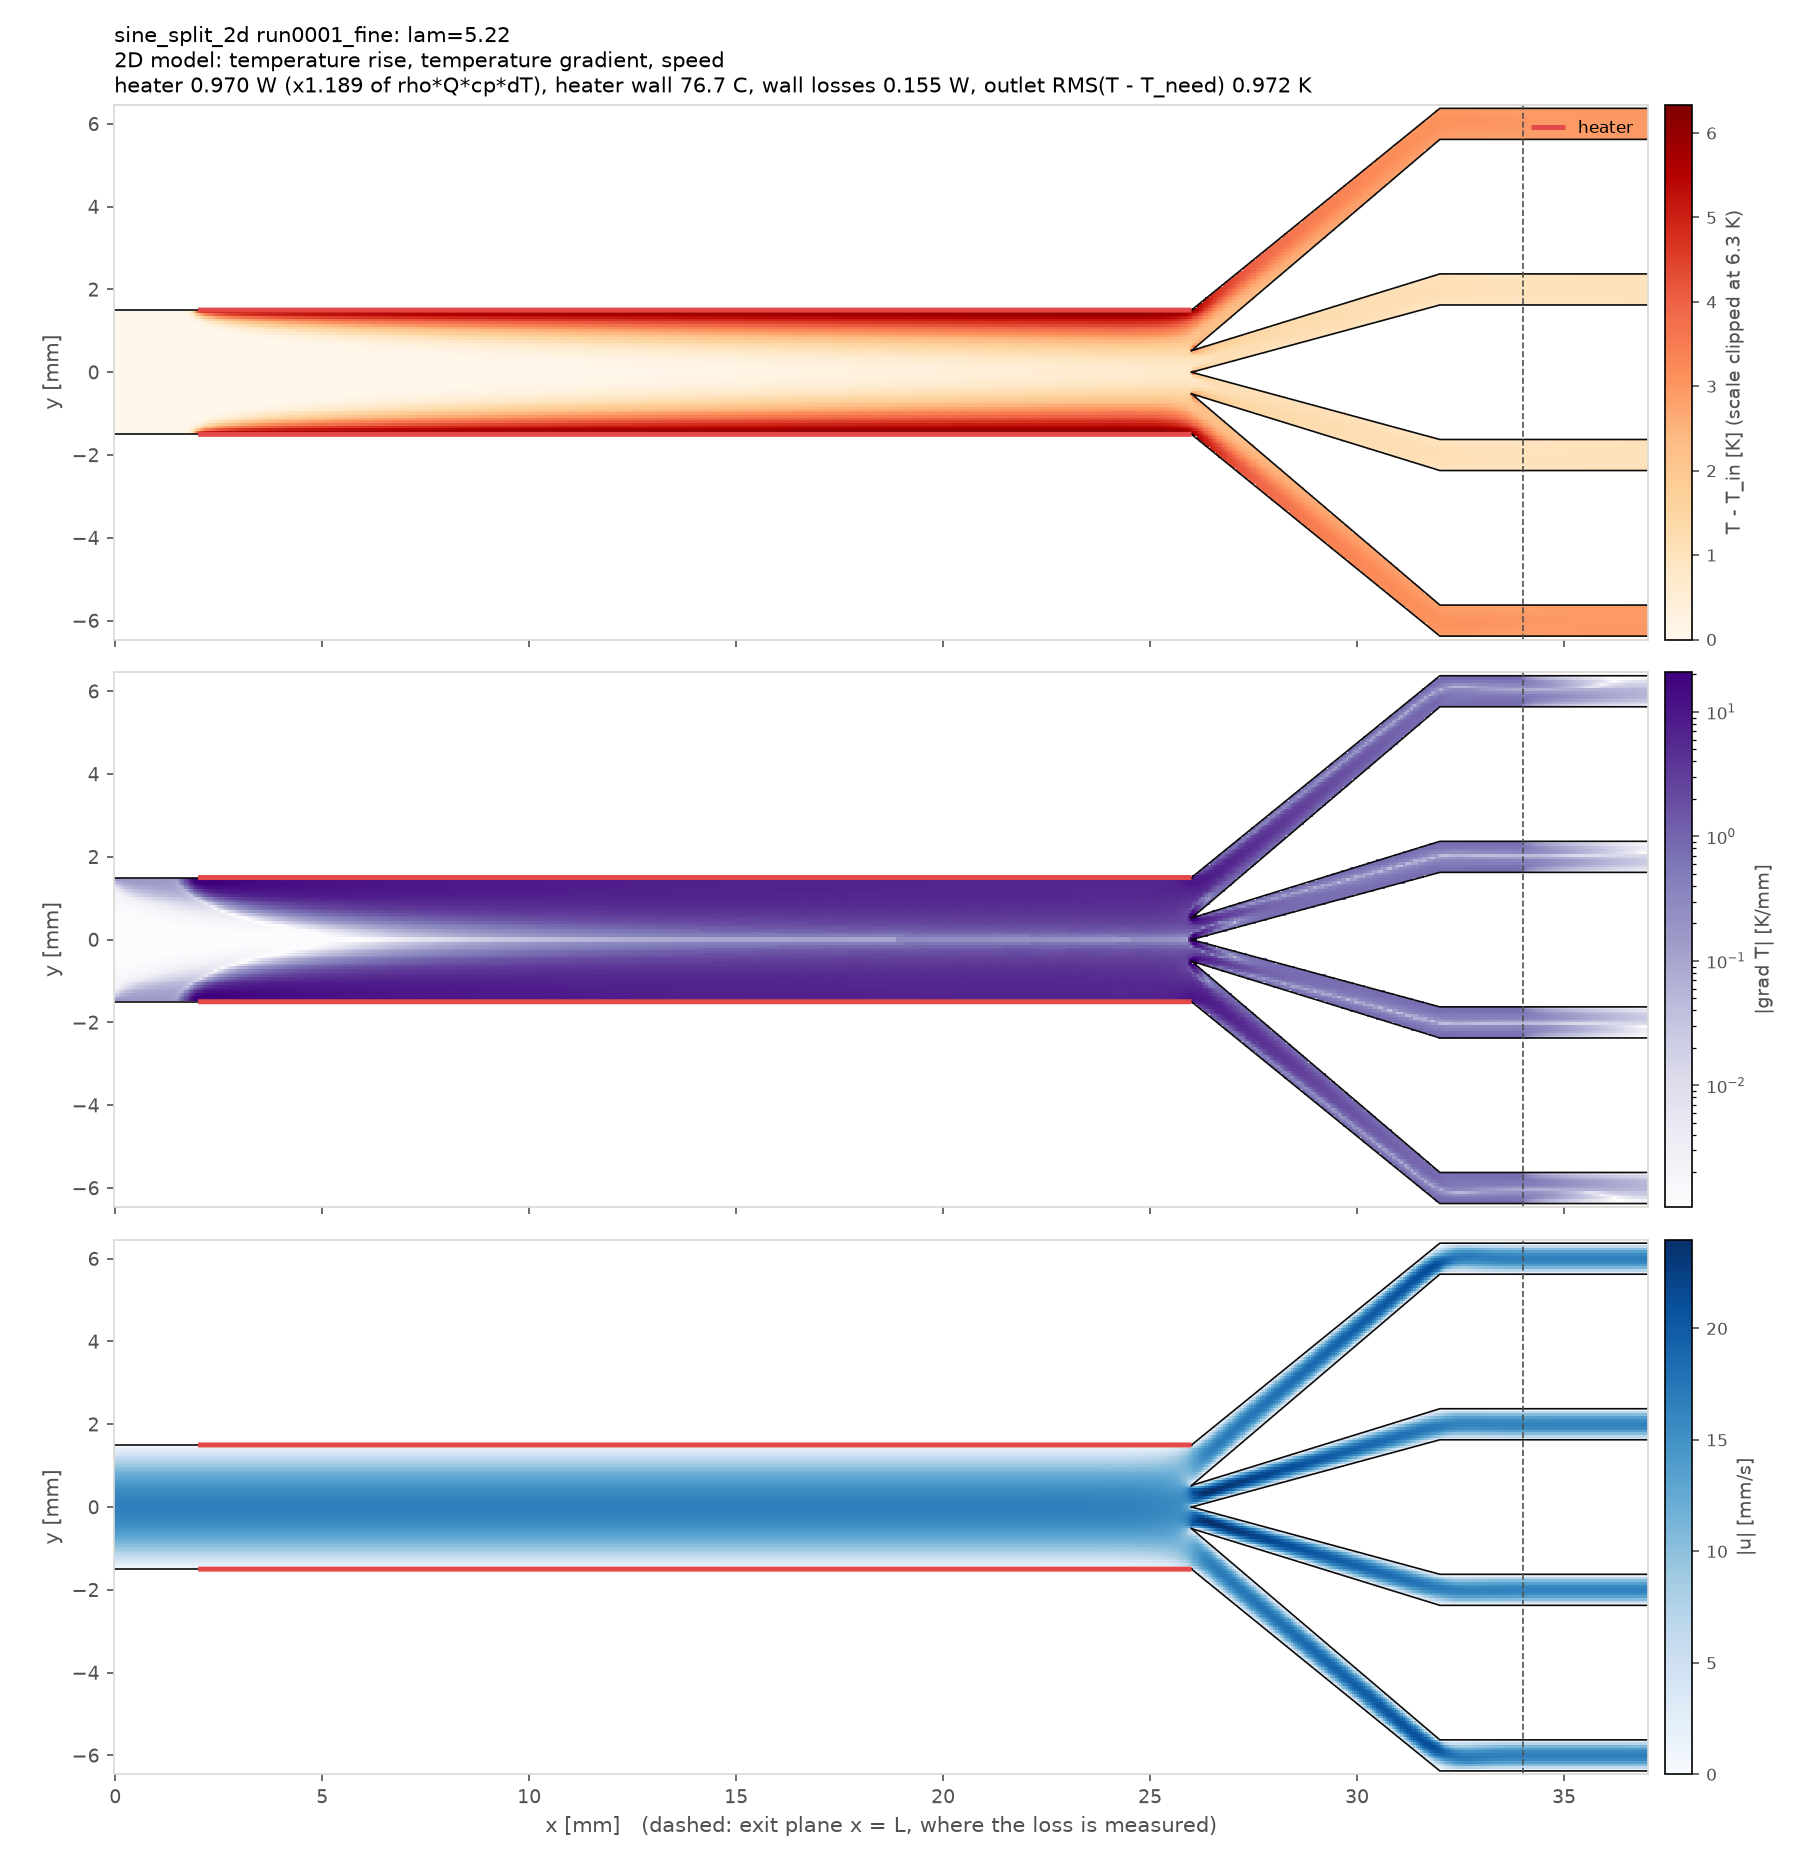
\includegraphics[width=0.95\textwidth,height=0.8\textheight,keepaspectratio]{runs/final_b2d_straight_ref_maps.png}
\caption{Temperature rise, temperature gradient and speed (mid-depth plane in 3D). Red: heated wall. The title's ``outlet RMS'' is the area-weighted $\ell_{2,\mathrm{area}}$.}
\end{figure}
\begin{figure}[H]\centering
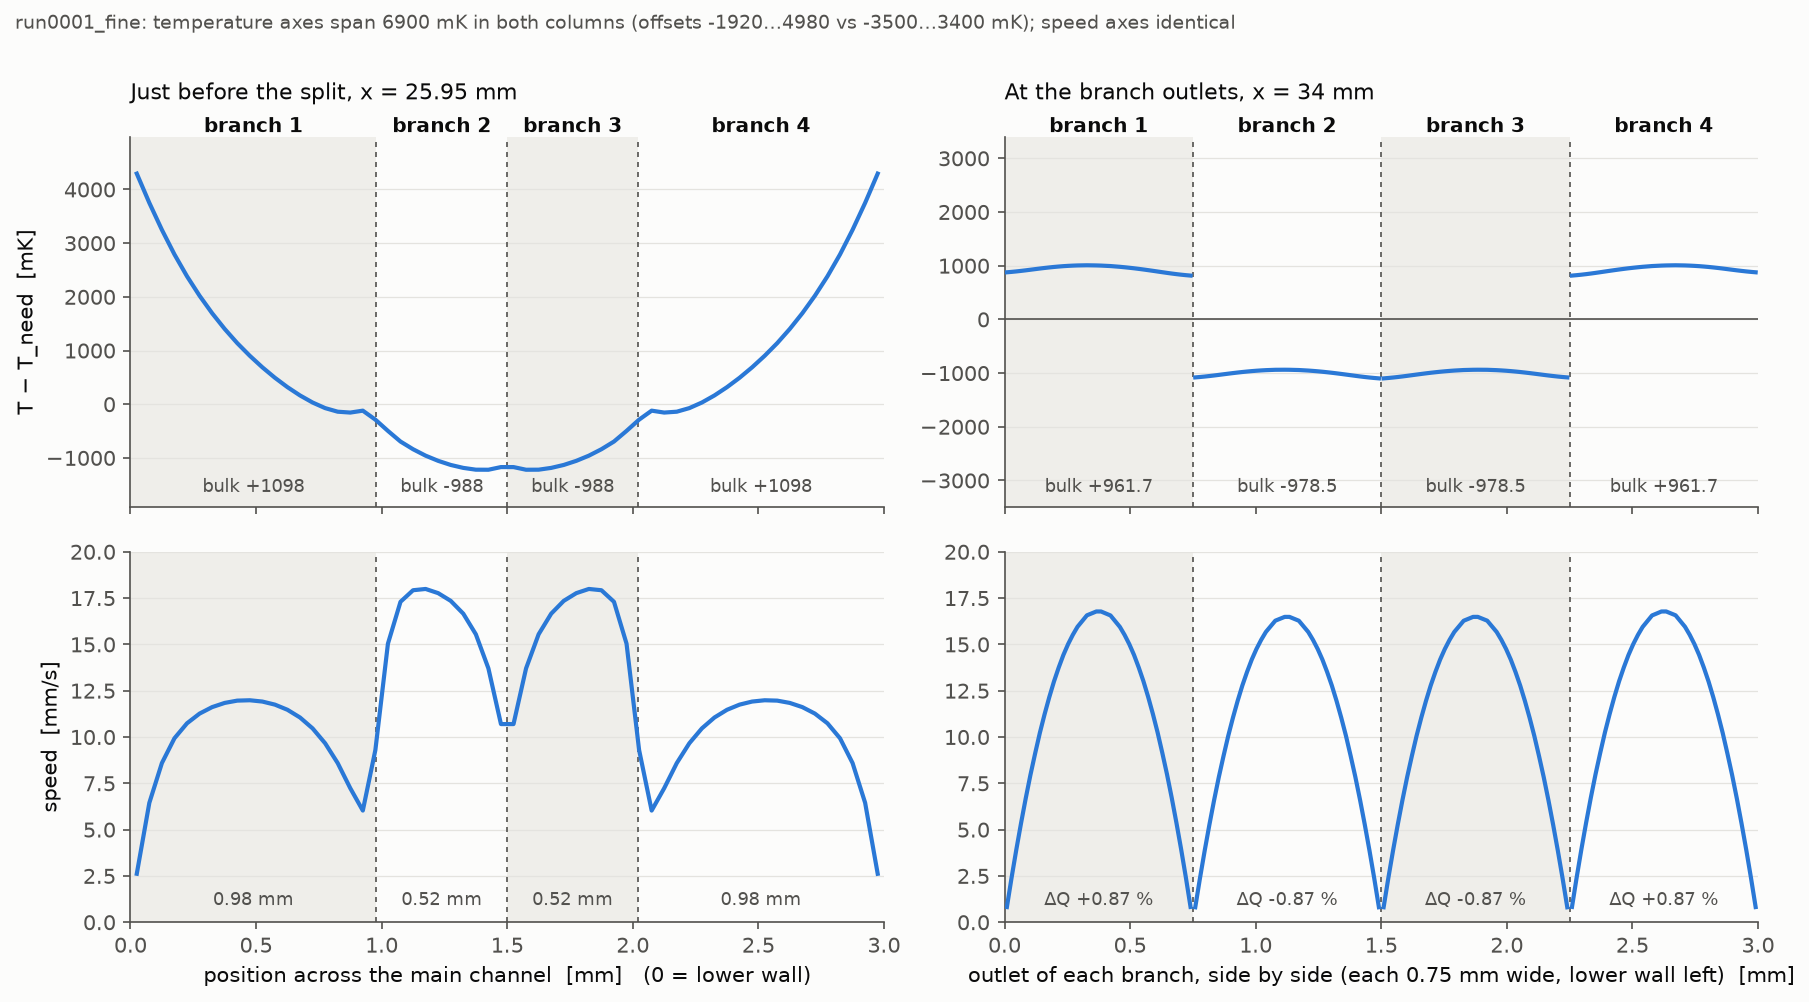
\includegraphics[width=0.95\textwidth,height=0.8\textheight,keepaspectratio]{runs/final_b2d_straight_ref_presplit.png}
\caption{Cross-section just before the split, cut into the four branch inlets, next to each branch outlet.}
\end{figure}
\begin{figure}[H]\centering
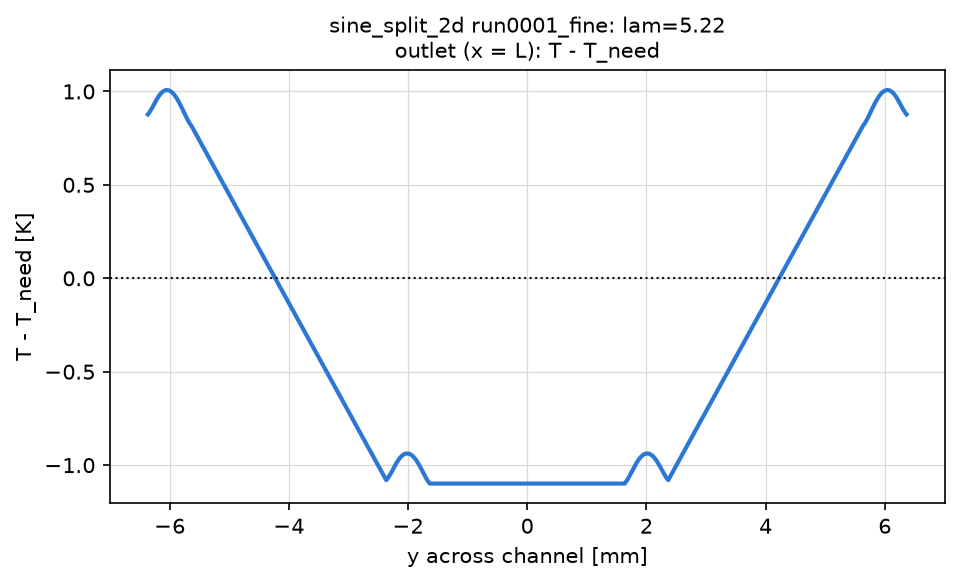
\includegraphics[width=0.75\textwidth,height=0.8\textheight,keepaspectratio]{runs/final_b2d_straight_ref_outlet.png}
\caption{Outlet temperature (and, in 3D, the outlet plane).}
\end{figure}
\begin{figure}[H]\centering
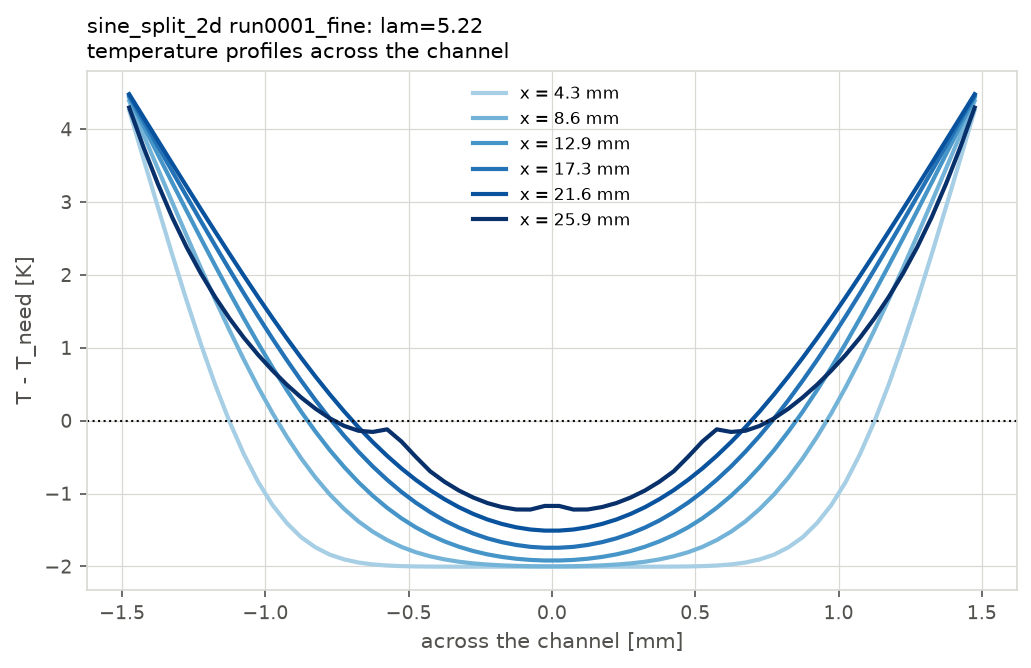
\includegraphics[width=0.62\textwidth,height=0.8\textheight,keepaspectratio]{runs/final_b2d_straight_ref_slices.png}
\caption{Temperature profiles across the channel at several $x$ stations.}
\end{figure}
\begin{figure}[H]\centering
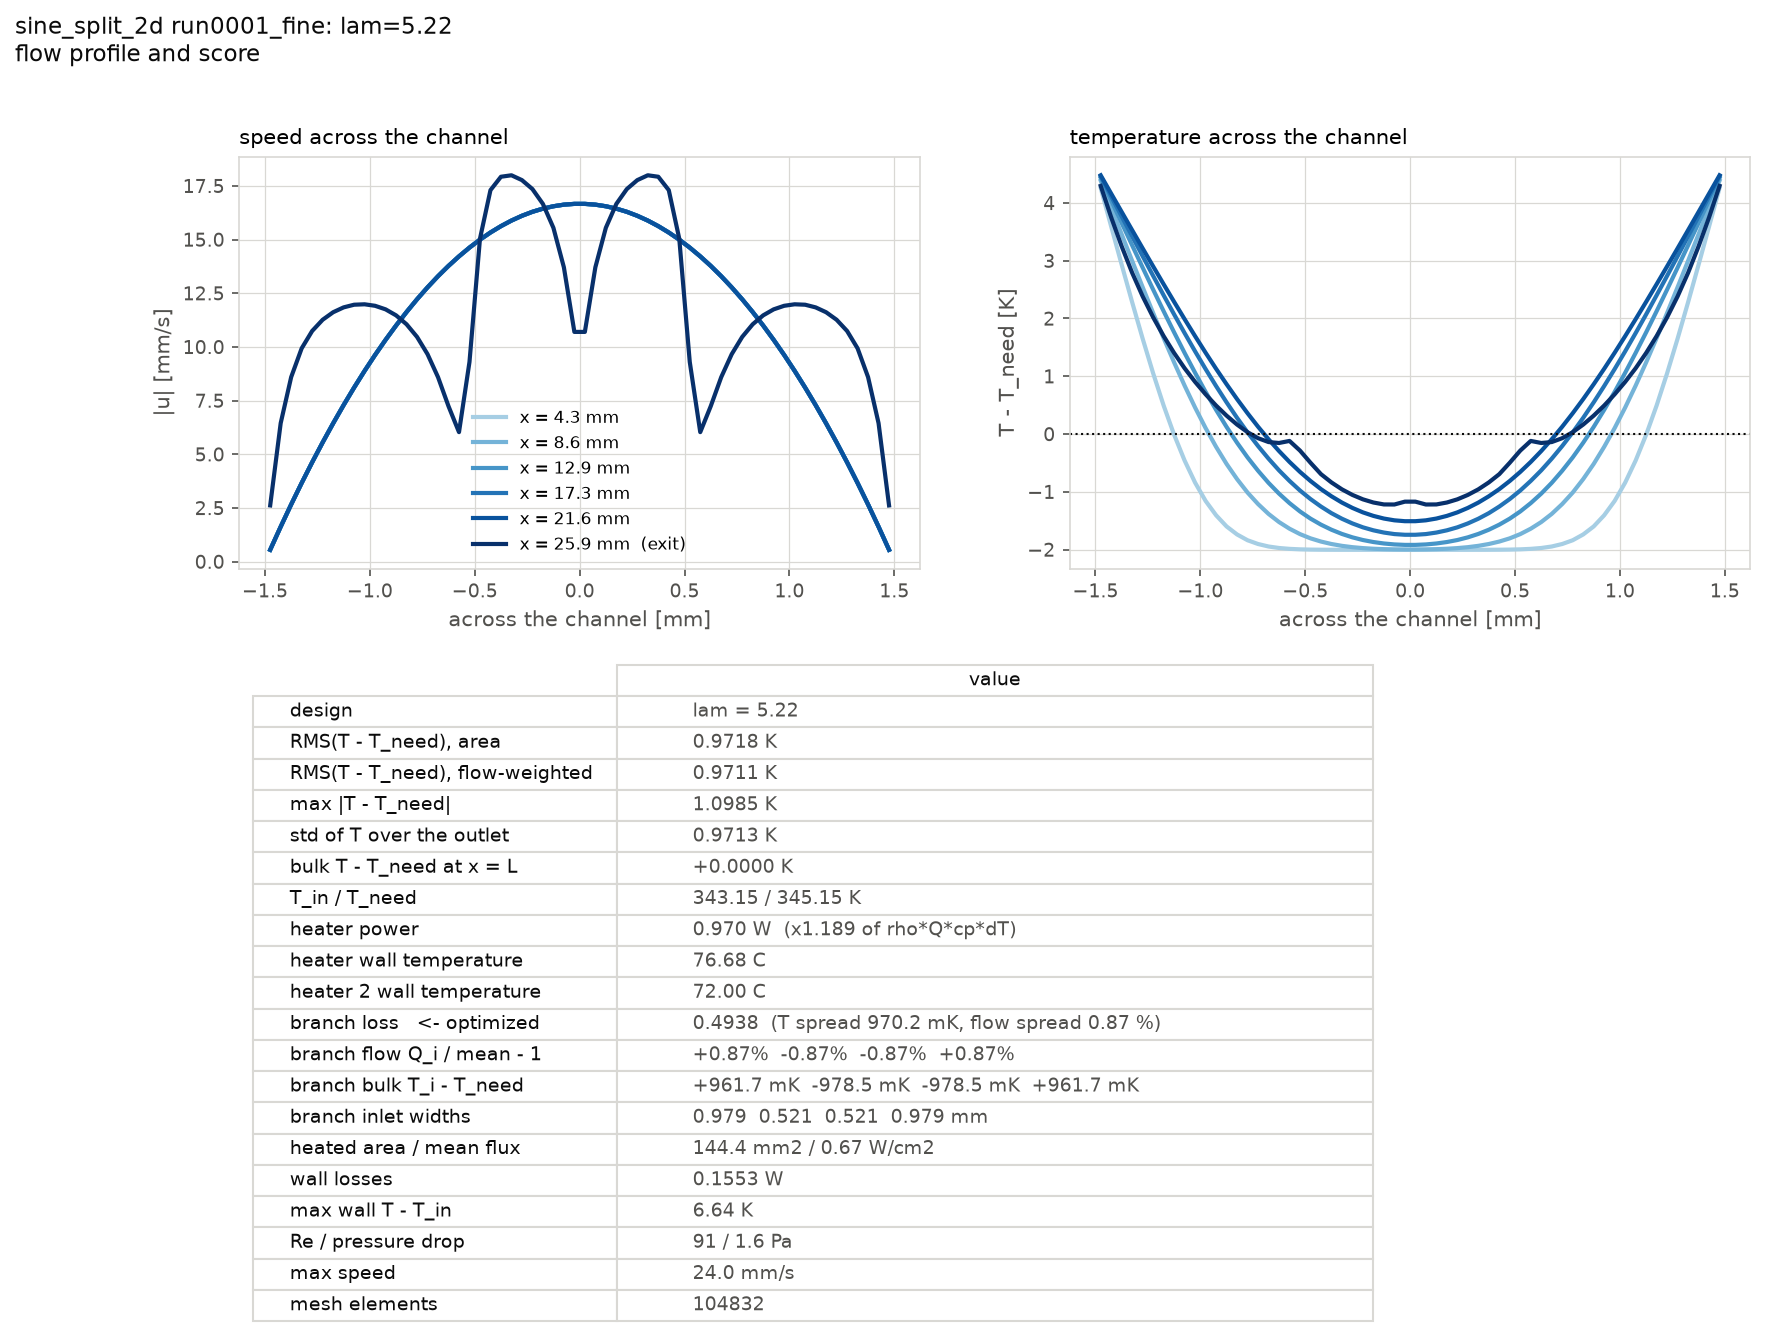
\includegraphics[width=0.8\textwidth,height=0.8\textheight,keepaspectratio]{runs/final_b2d_straight_ref_profile.png}
\caption{Speed and temperature across the channel at several $x$ stations, and the full score table of the design.}
\end{figure}
\begin{figure}[H]\centering
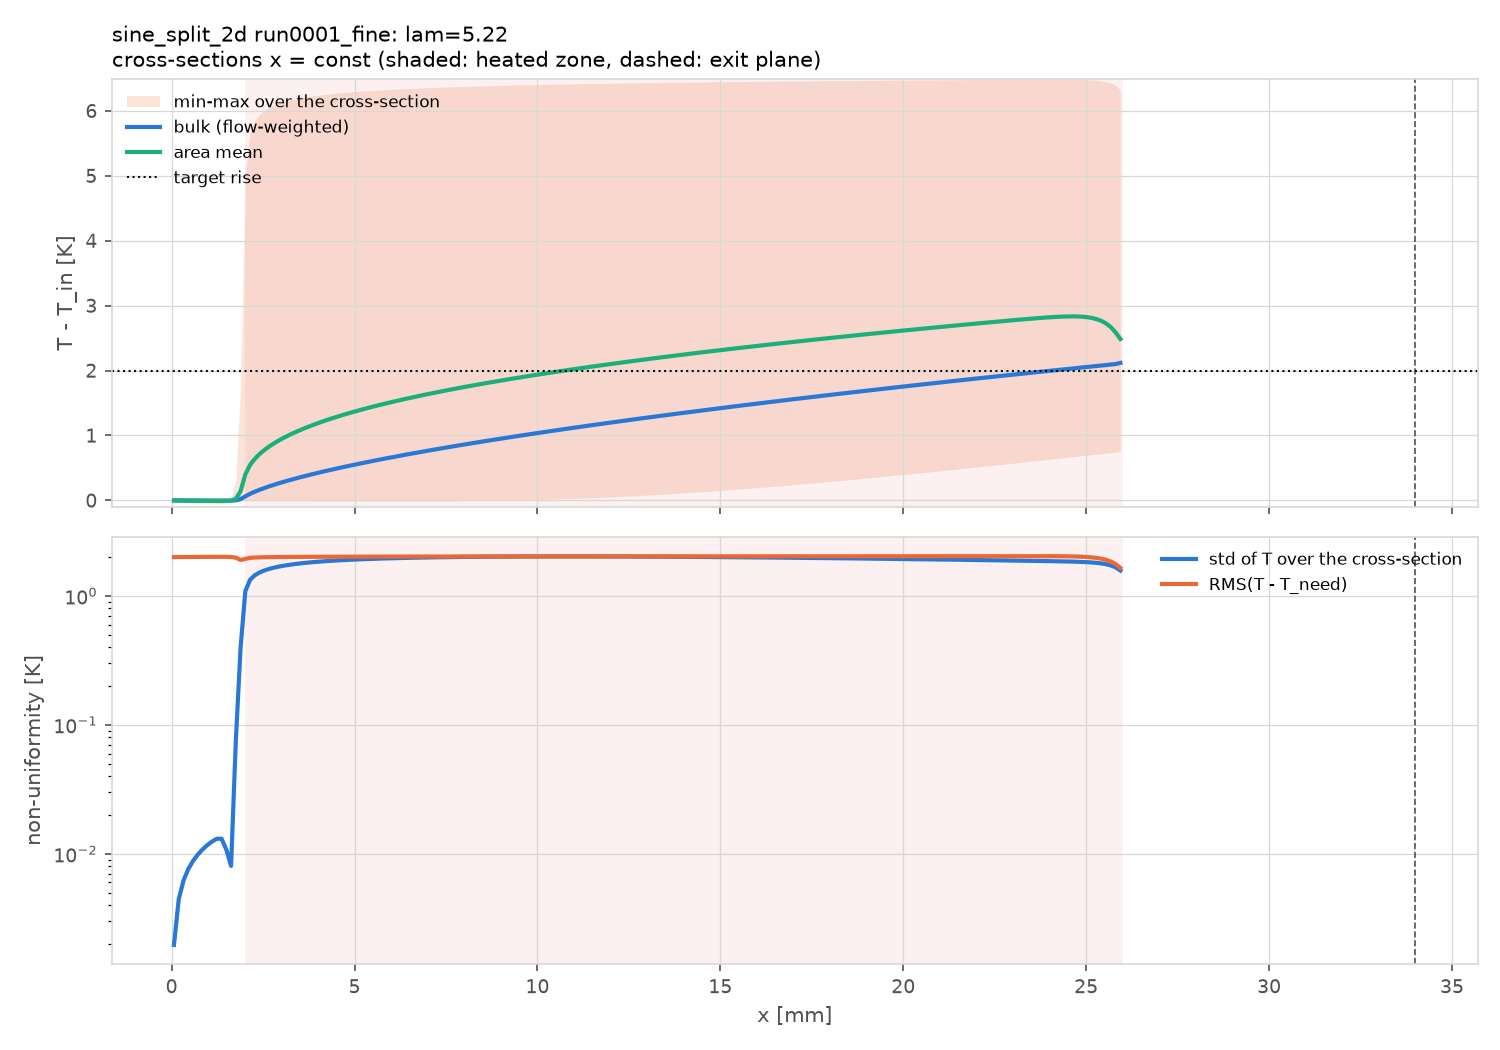
\includegraphics[width=0.8\textwidth,height=0.8\textheight,keepaspectratio]{runs/final_b2d_straight_ref_along_x.png}
\caption{Bulk, mean, min and max temperature along the channel.}
\end{figure}
\clearpage
\subsubsection*{Branched straight, BO best \#16 ($\rho$ 0.540, heater 2.4\mm, clamped at 99\,$^\circ$C): 515\mK, 0.16\,\%}
\noindent\texttt{runs/final\_b2d\_straight}\par\medskip
\begin{figure}[H]\centering
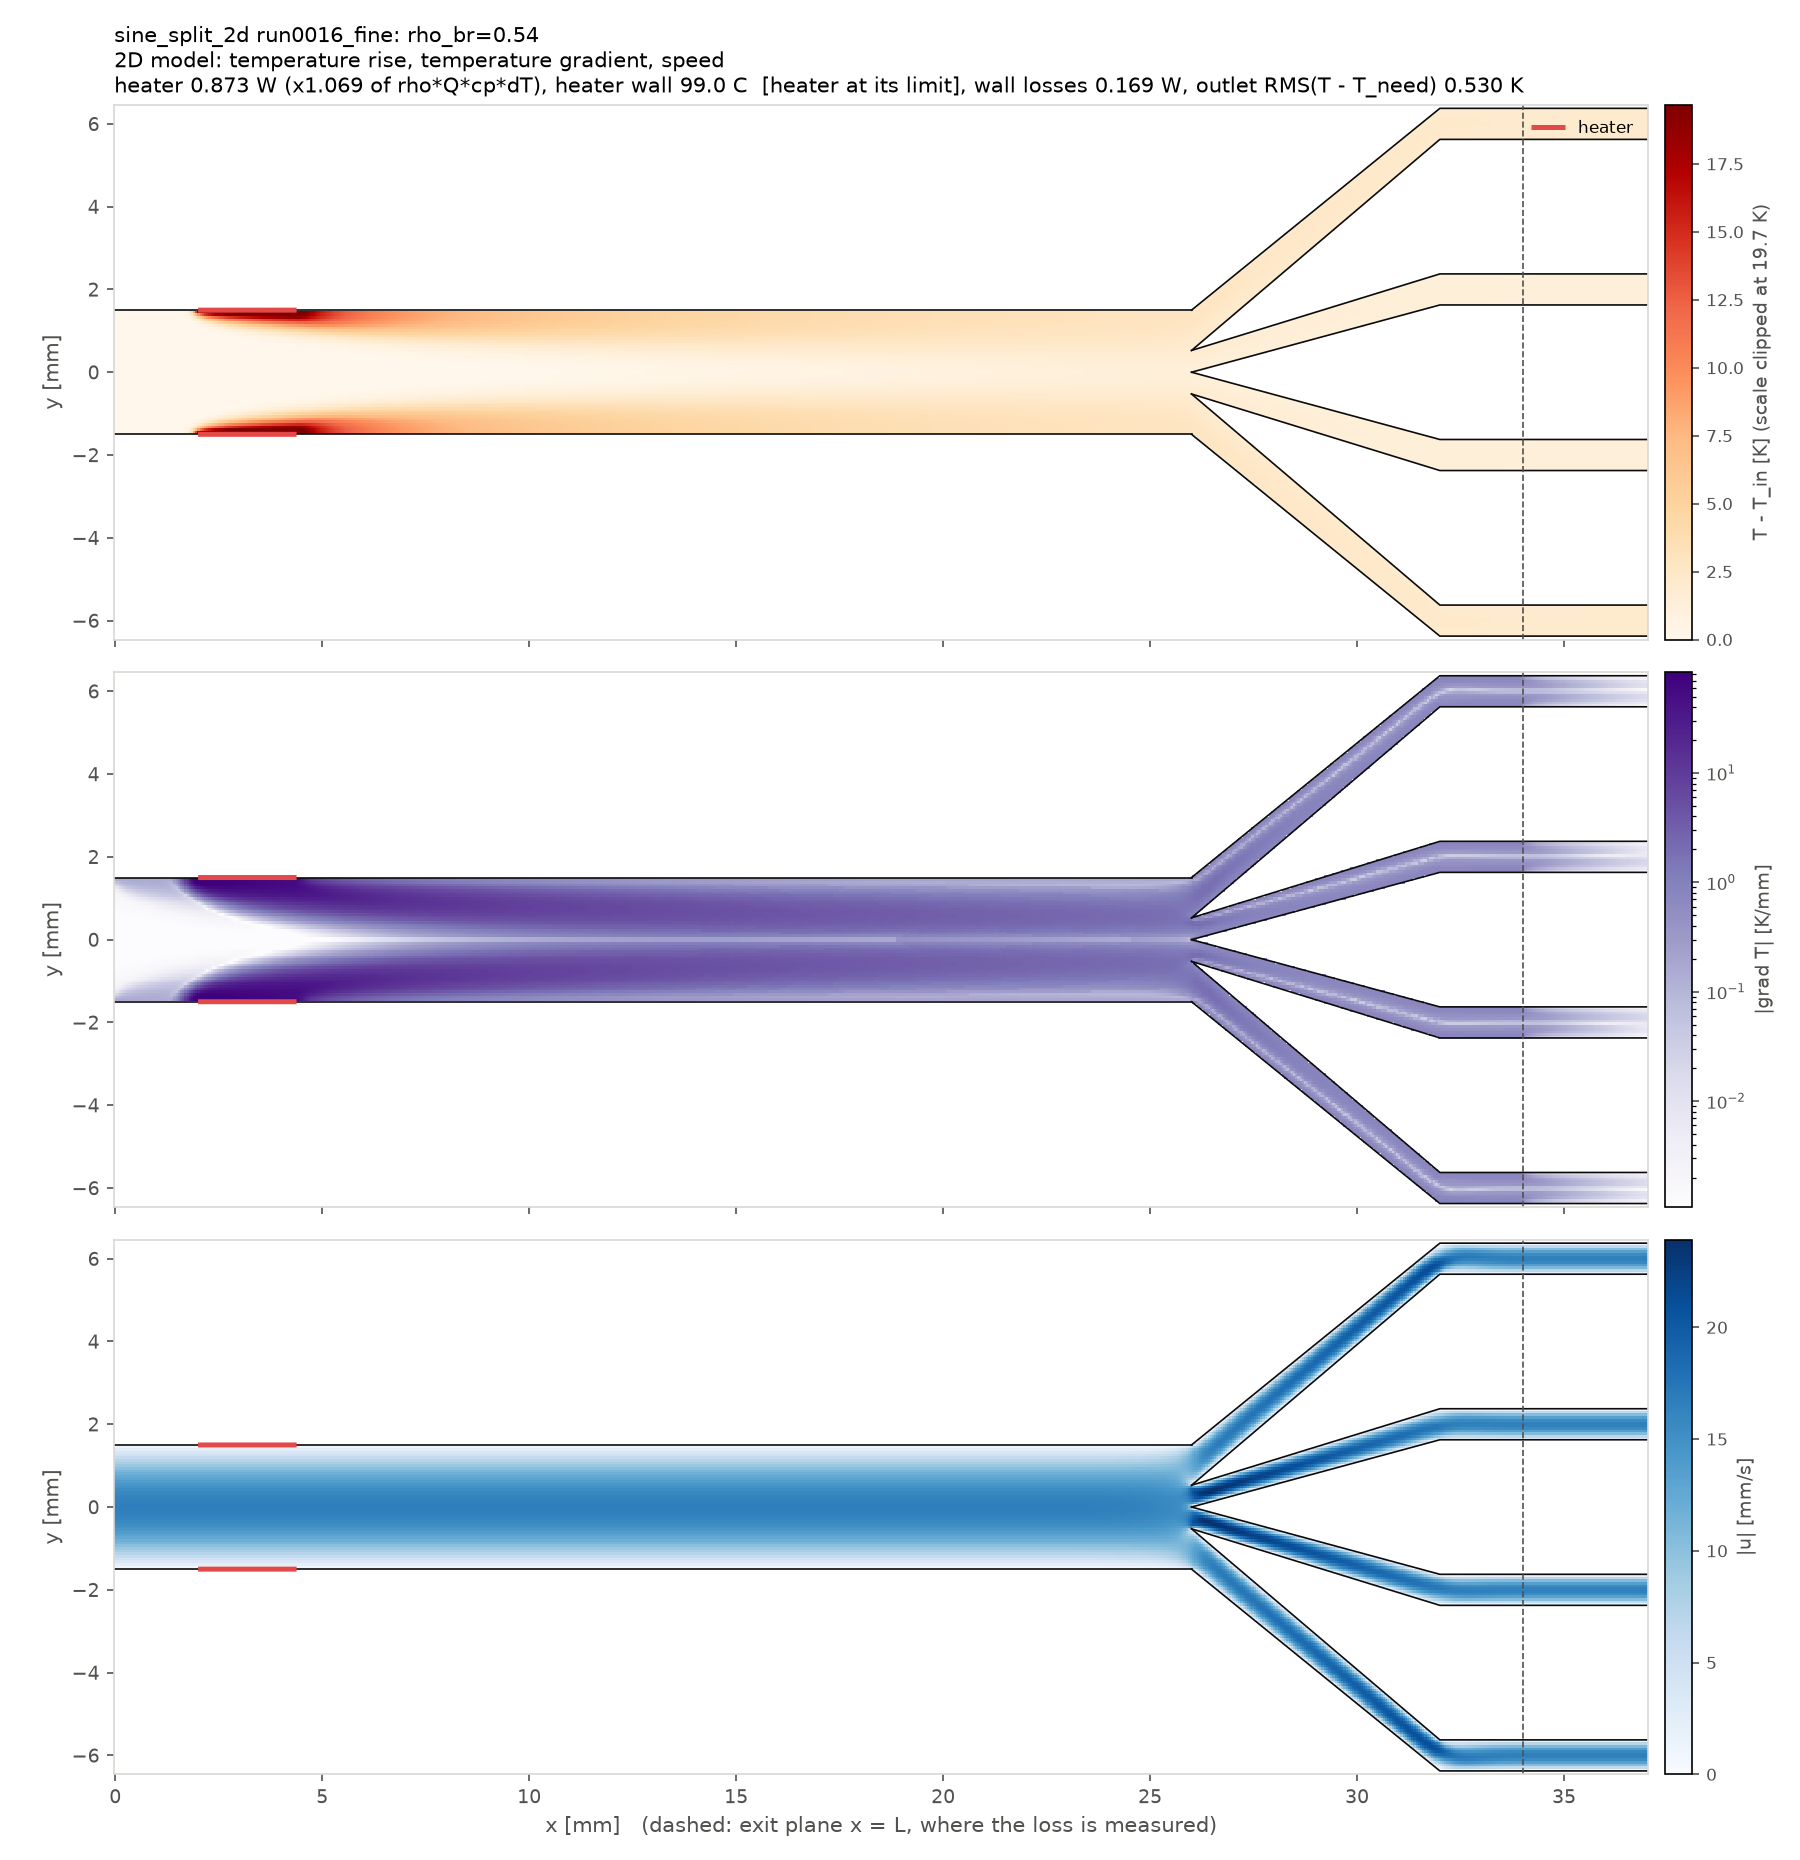
\includegraphics[width=0.95\textwidth,height=0.8\textheight,keepaspectratio]{runs/final_b2d_straight_maps.png}
\caption{Temperature rise, temperature gradient and speed (mid-depth plane in 3D). Red: heated wall. The title's ``outlet RMS'' is the area-weighted $\ell_{2,\mathrm{area}}$.}
\end{figure}
\begin{figure}[H]\centering
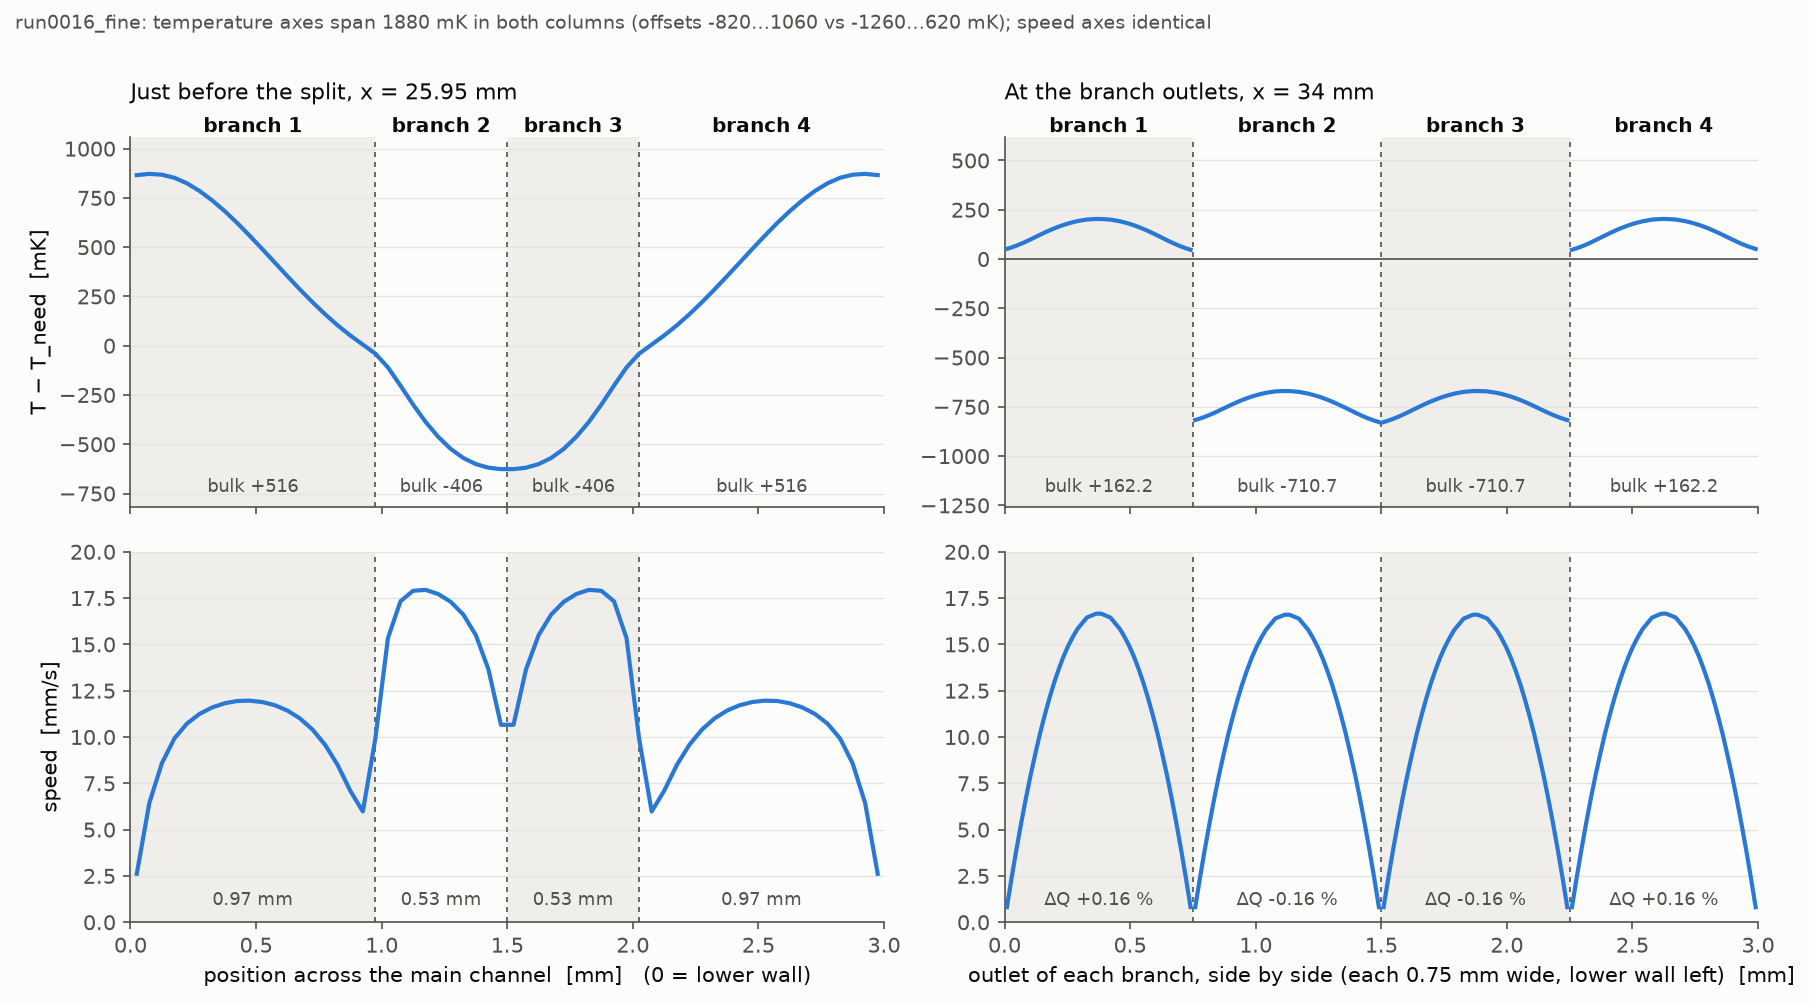
\includegraphics[width=0.95\textwidth,height=0.8\textheight,keepaspectratio]{runs/final_b2d_straight_presplit.png}
\caption{Cross-section just before the split, cut into the four branch inlets, next to each branch outlet.}
\end{figure}
\begin{figure}[H]\centering
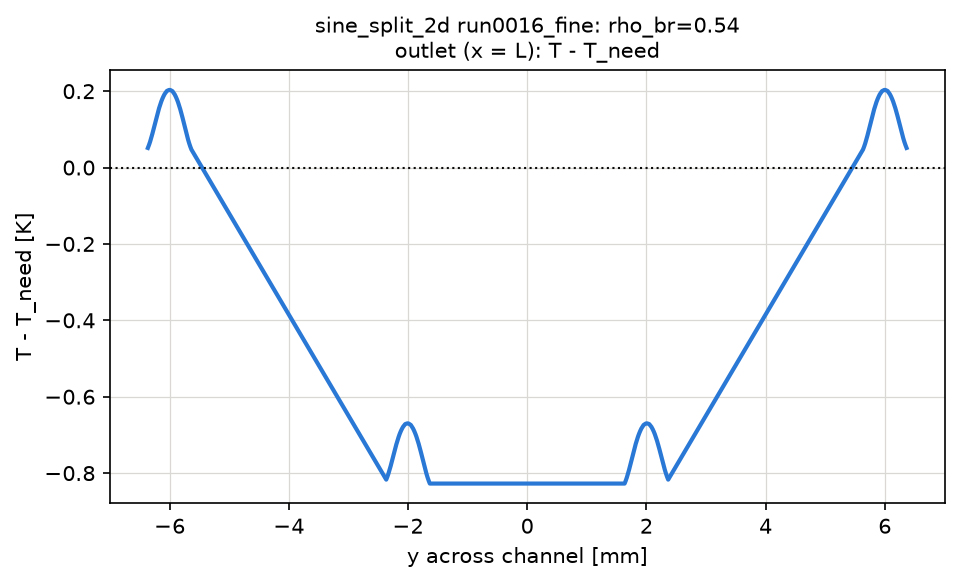
\includegraphics[width=0.75\textwidth,height=0.8\textheight,keepaspectratio]{runs/final_b2d_straight_outlet.png}
\caption{Outlet temperature (and, in 3D, the outlet plane).}
\end{figure}
\begin{figure}[H]\centering
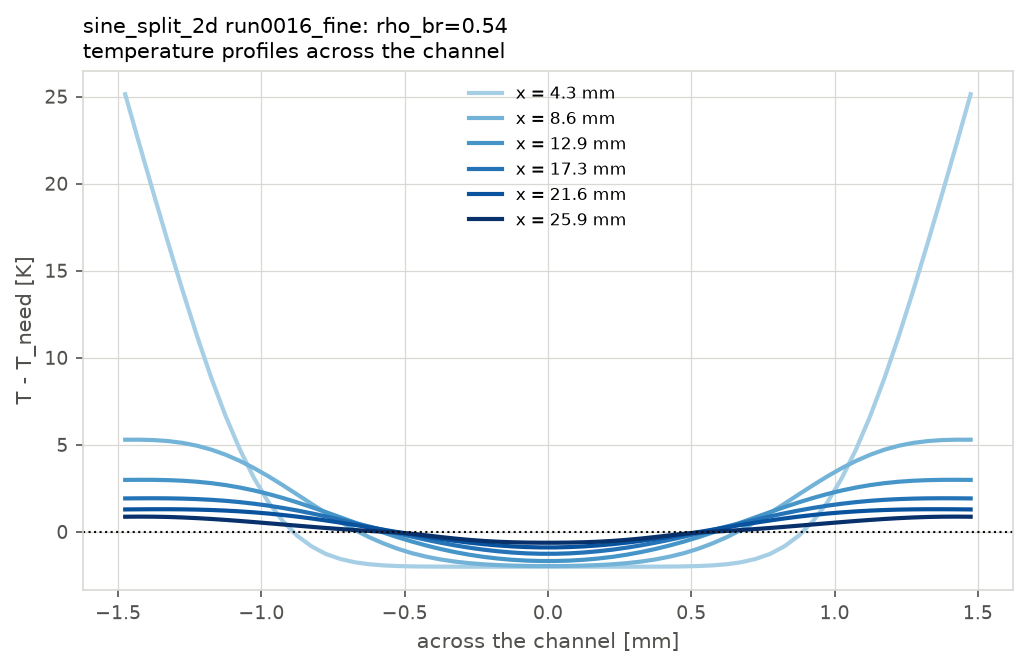
\includegraphics[width=0.62\textwidth,height=0.8\textheight,keepaspectratio]{runs/final_b2d_straight_slices.png}
\caption{Temperature profiles across the channel at several $x$ stations.}
\end{figure}
\begin{figure}[H]\centering
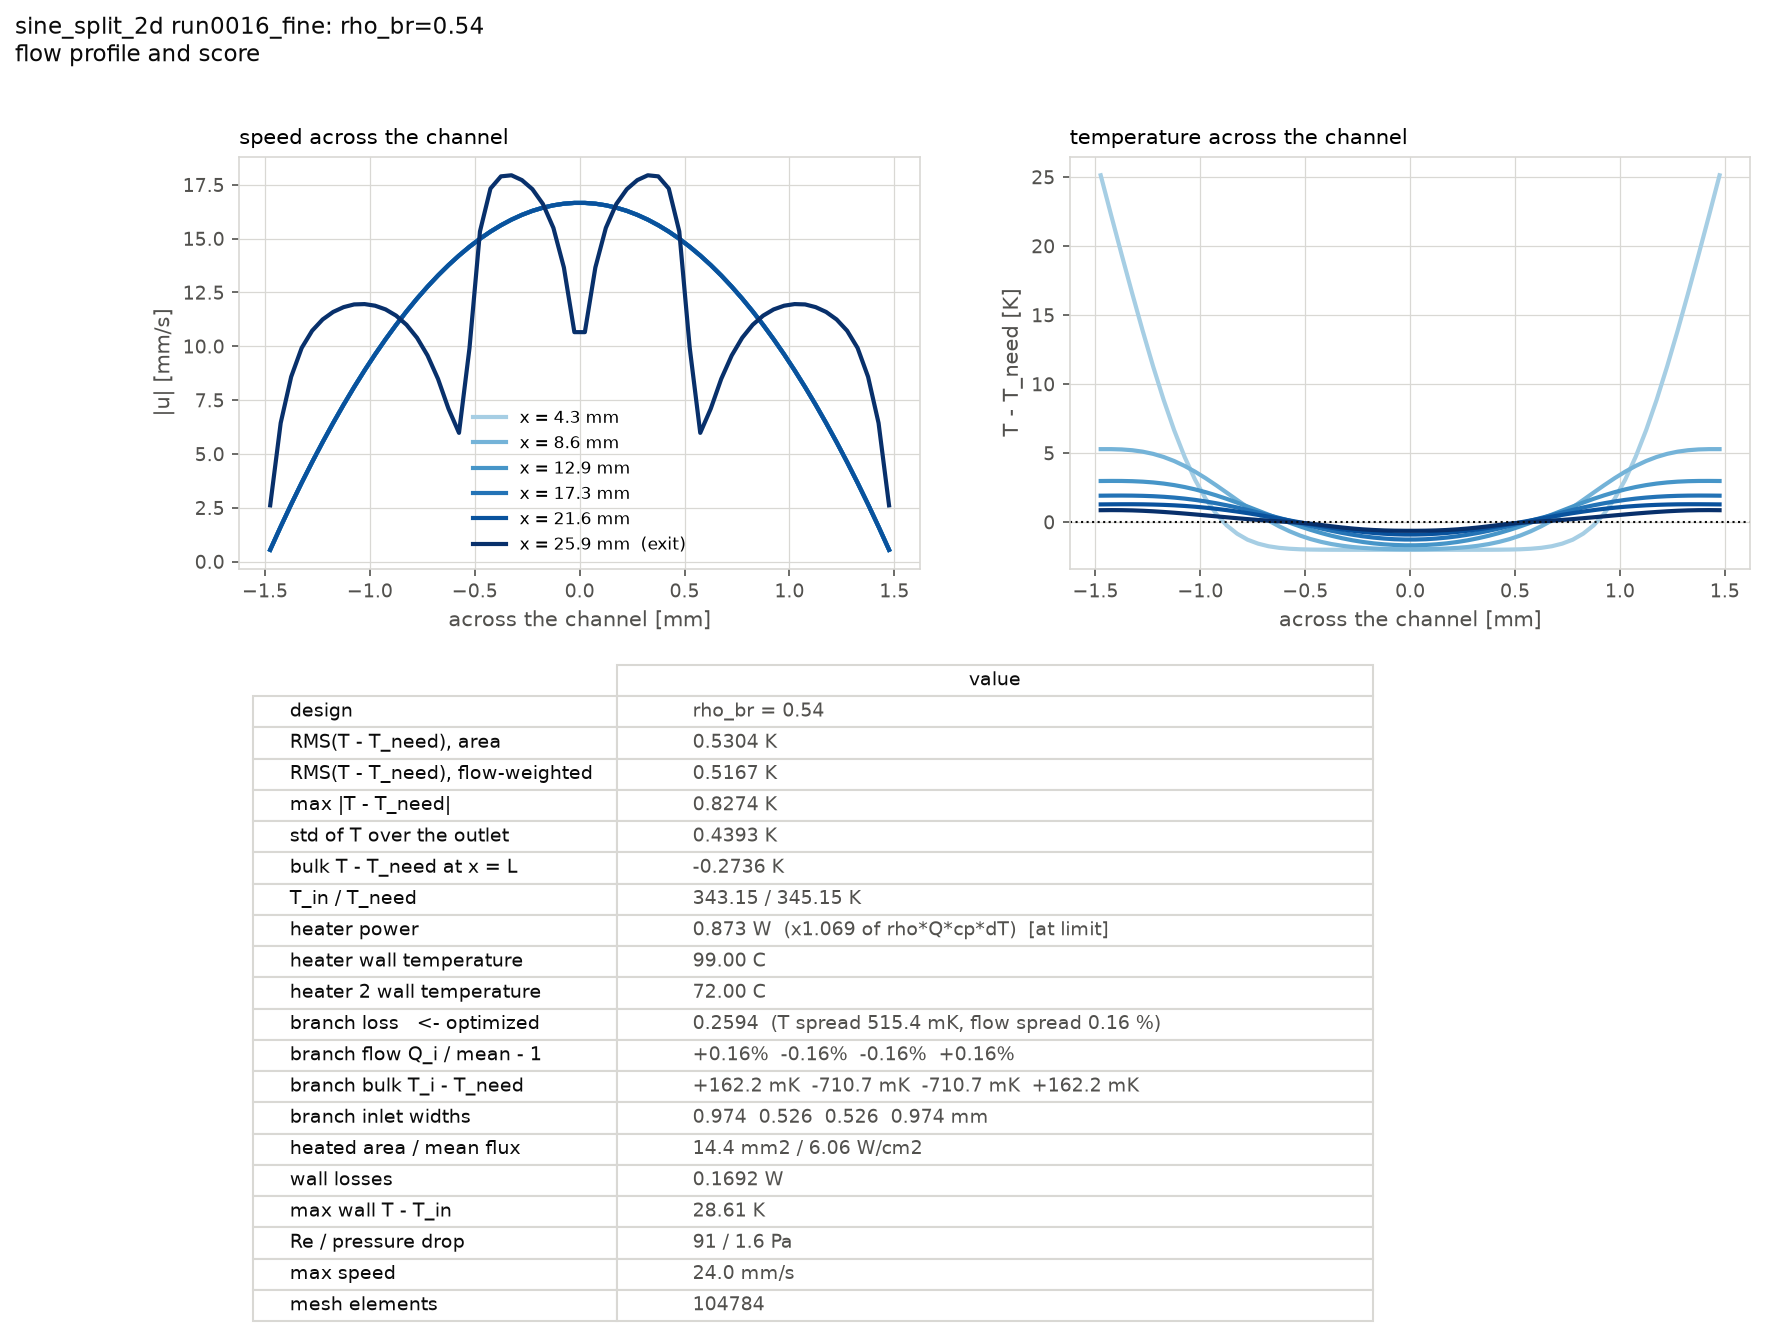
\includegraphics[width=0.8\textwidth,height=0.8\textheight,keepaspectratio]{runs/final_b2d_straight_profile.png}
\caption{Speed and temperature across the channel at several $x$ stations, and the full score table of the design.}
\end{figure}
\begin{figure}[H]\centering
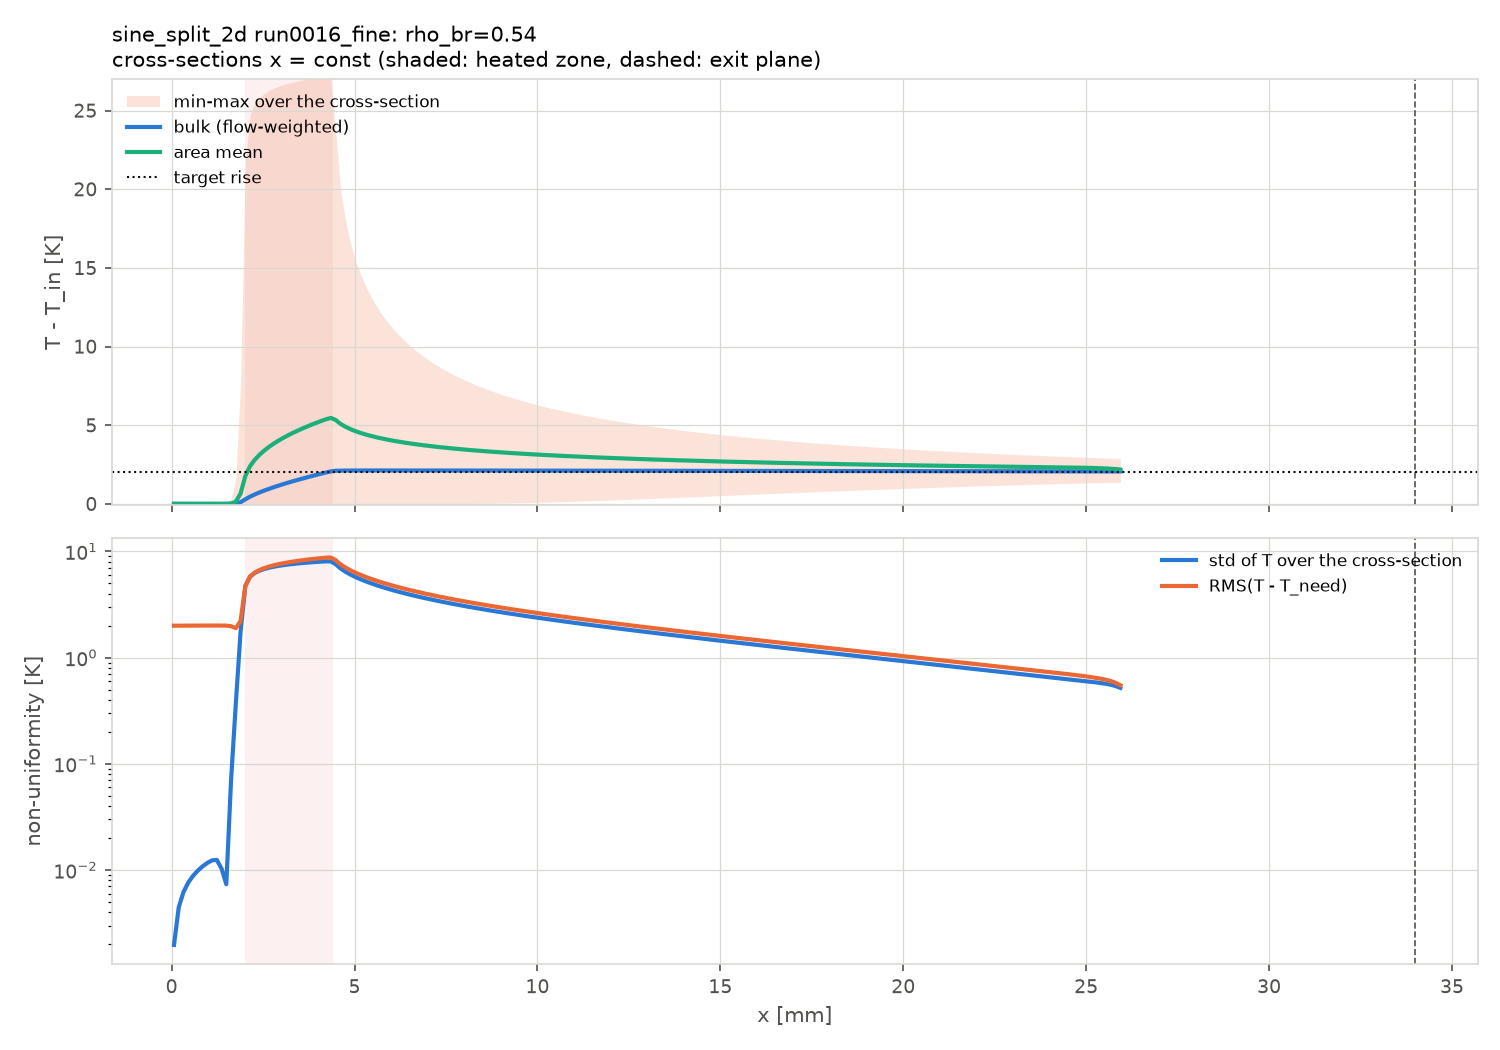
\includegraphics[width=0.8\textwidth,height=0.8\textheight,keepaspectratio]{runs/final_b2d_straight_along_x.png}
\caption{Bulk, mean, min and max temperature along the channel.}
\end{figure}
\begin{figure}[H]\centering
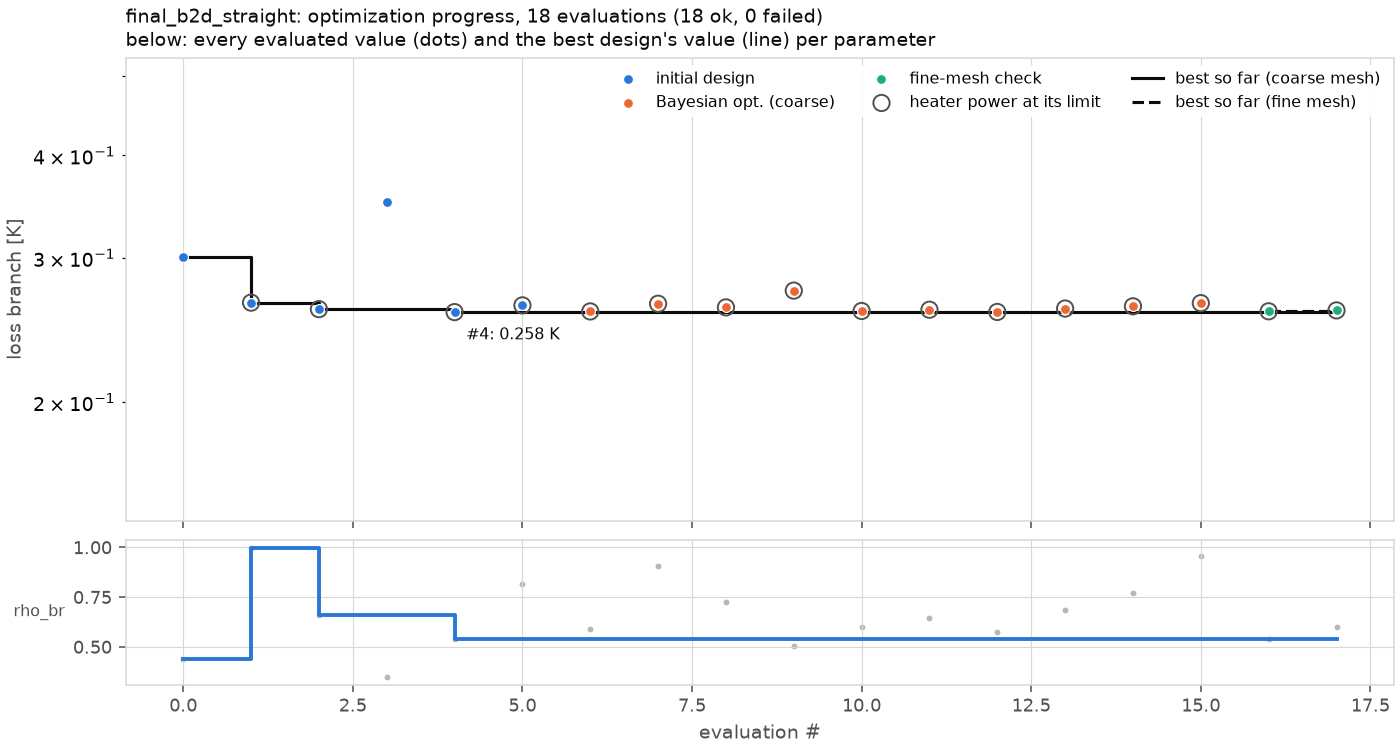
\includegraphics[width=0.85\textwidth]{runs/final_b2d_straight_progress_loss.png}
\caption{Search history: loss of every evaluation, best so far, and the parameters.}
\end{figure}
\clearpage
\subsubsection*{Branched sine + straight, BO best \#150: 116\mK, 0.82\,\%}
\noindent\texttt{runs/final\_b2d\_sine}\par\medskip
\begin{figure}[H]\centering
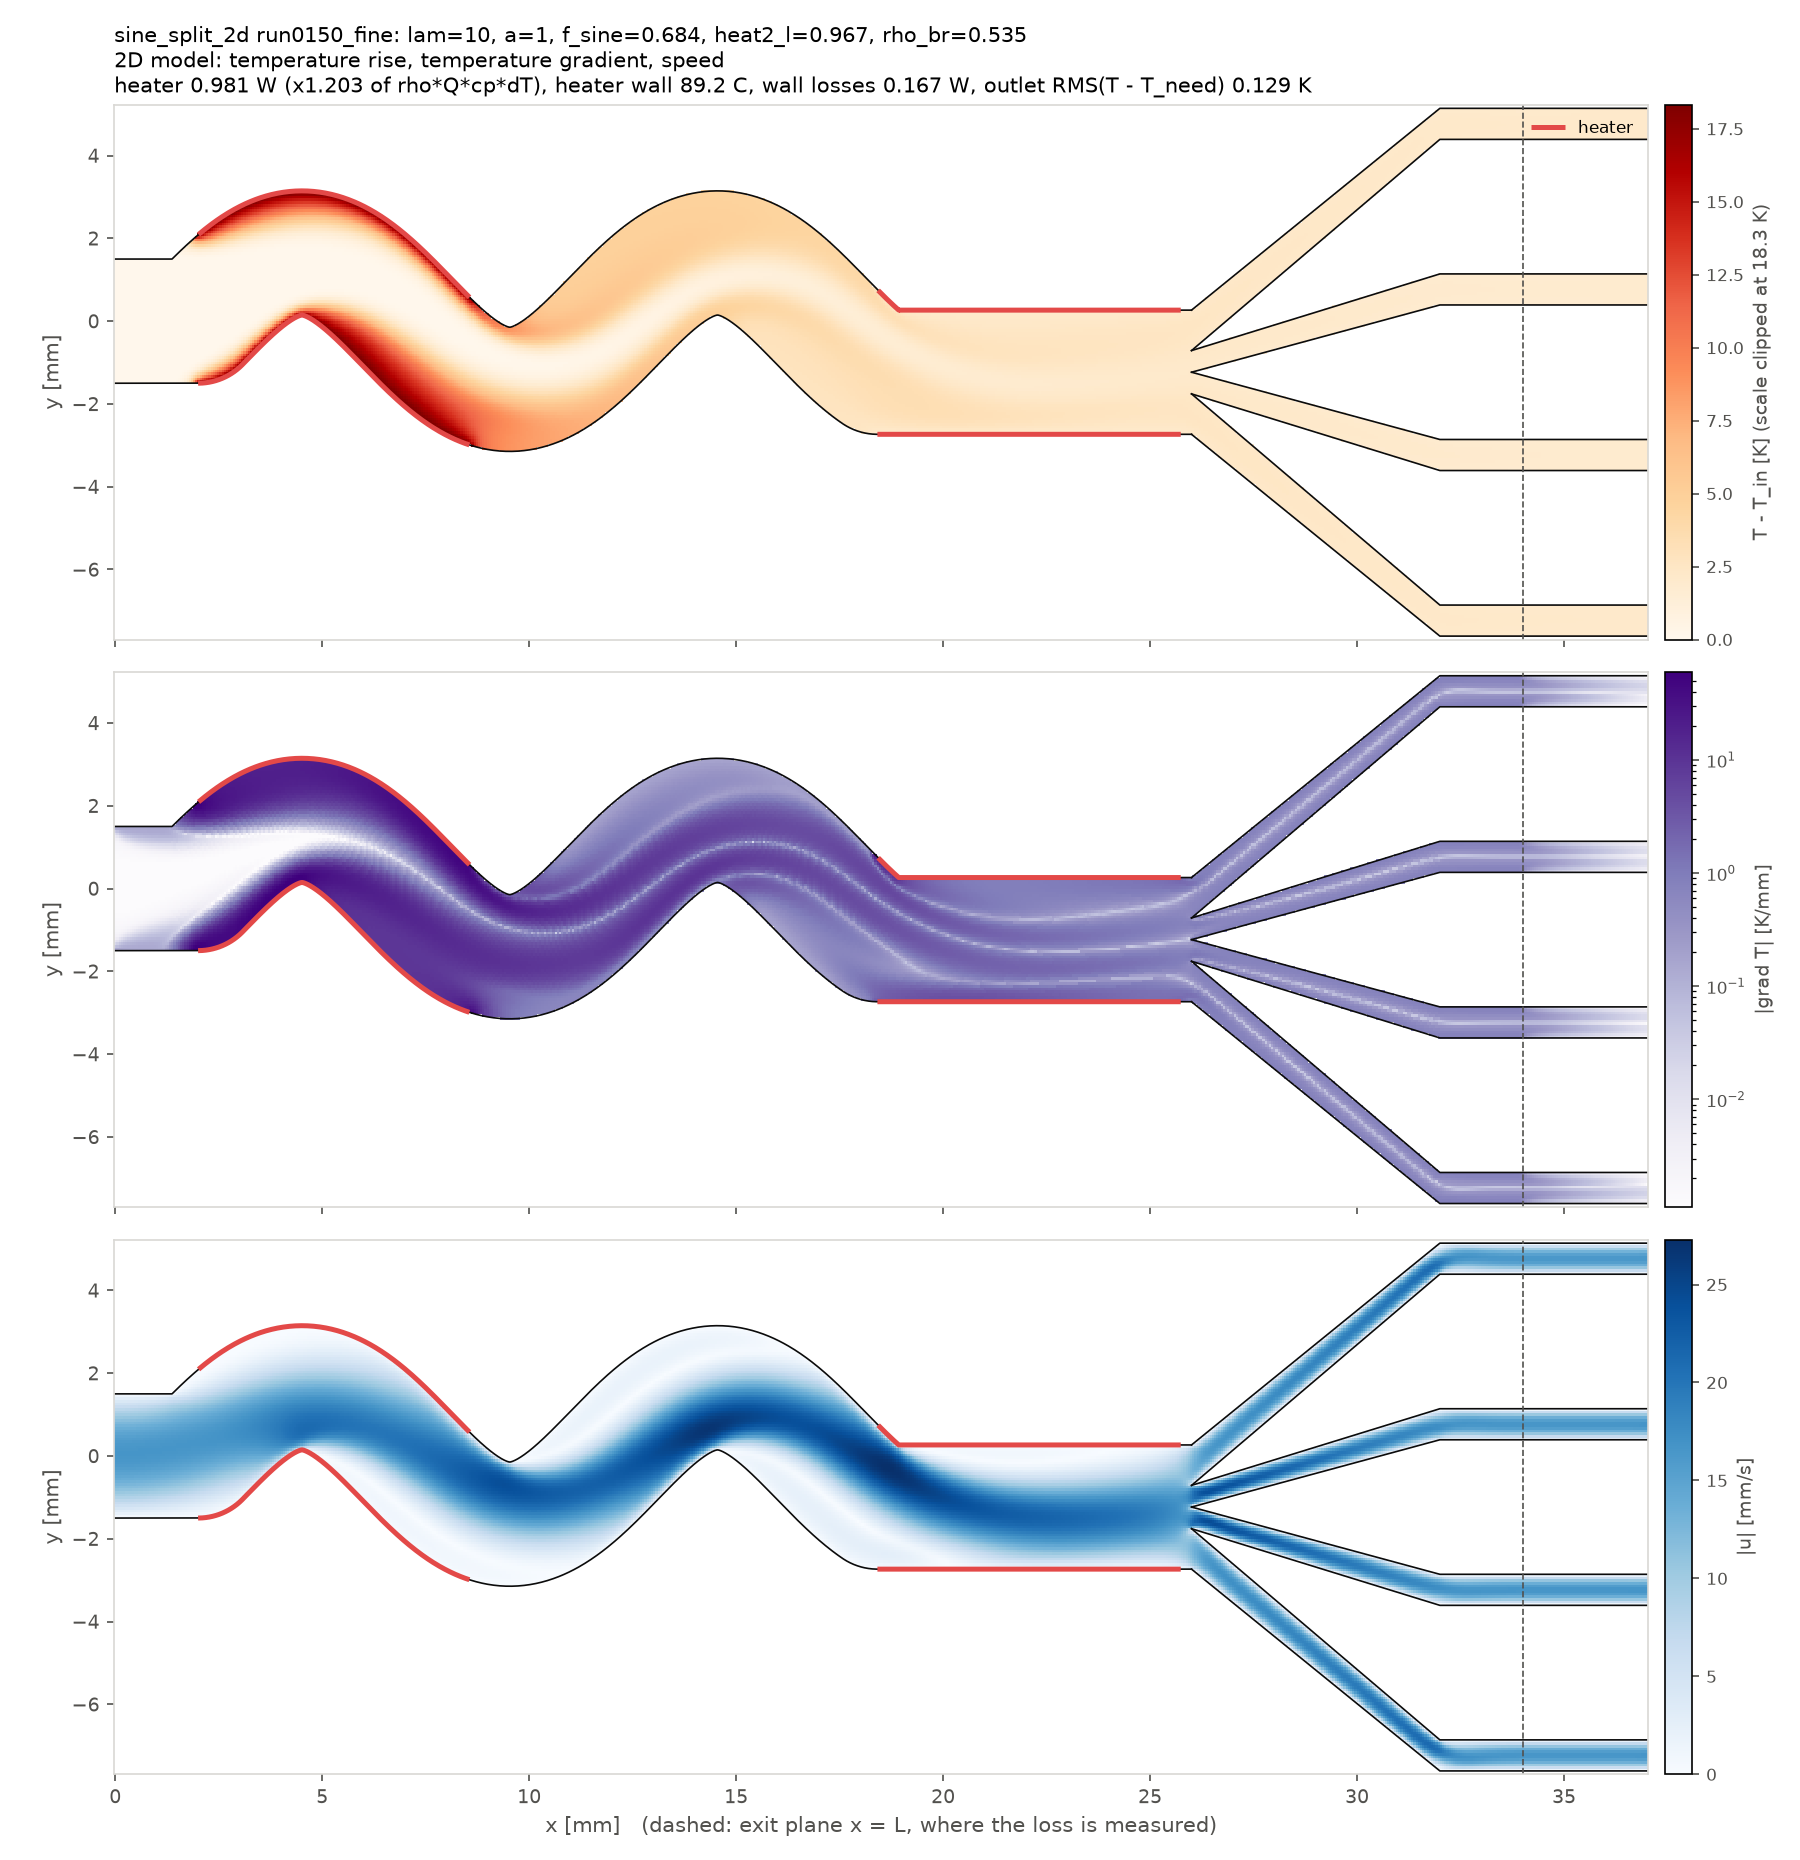
\includegraphics[width=0.95\textwidth,height=0.8\textheight,keepaspectratio]{runs/final_b2d_sine_maps.png}
\caption{Temperature rise, temperature gradient and speed (mid-depth plane in 3D). Red: heated wall. The title's ``outlet RMS'' is the area-weighted $\ell_{2,\mathrm{area}}$.}
\end{figure}
\begin{figure}[H]\centering
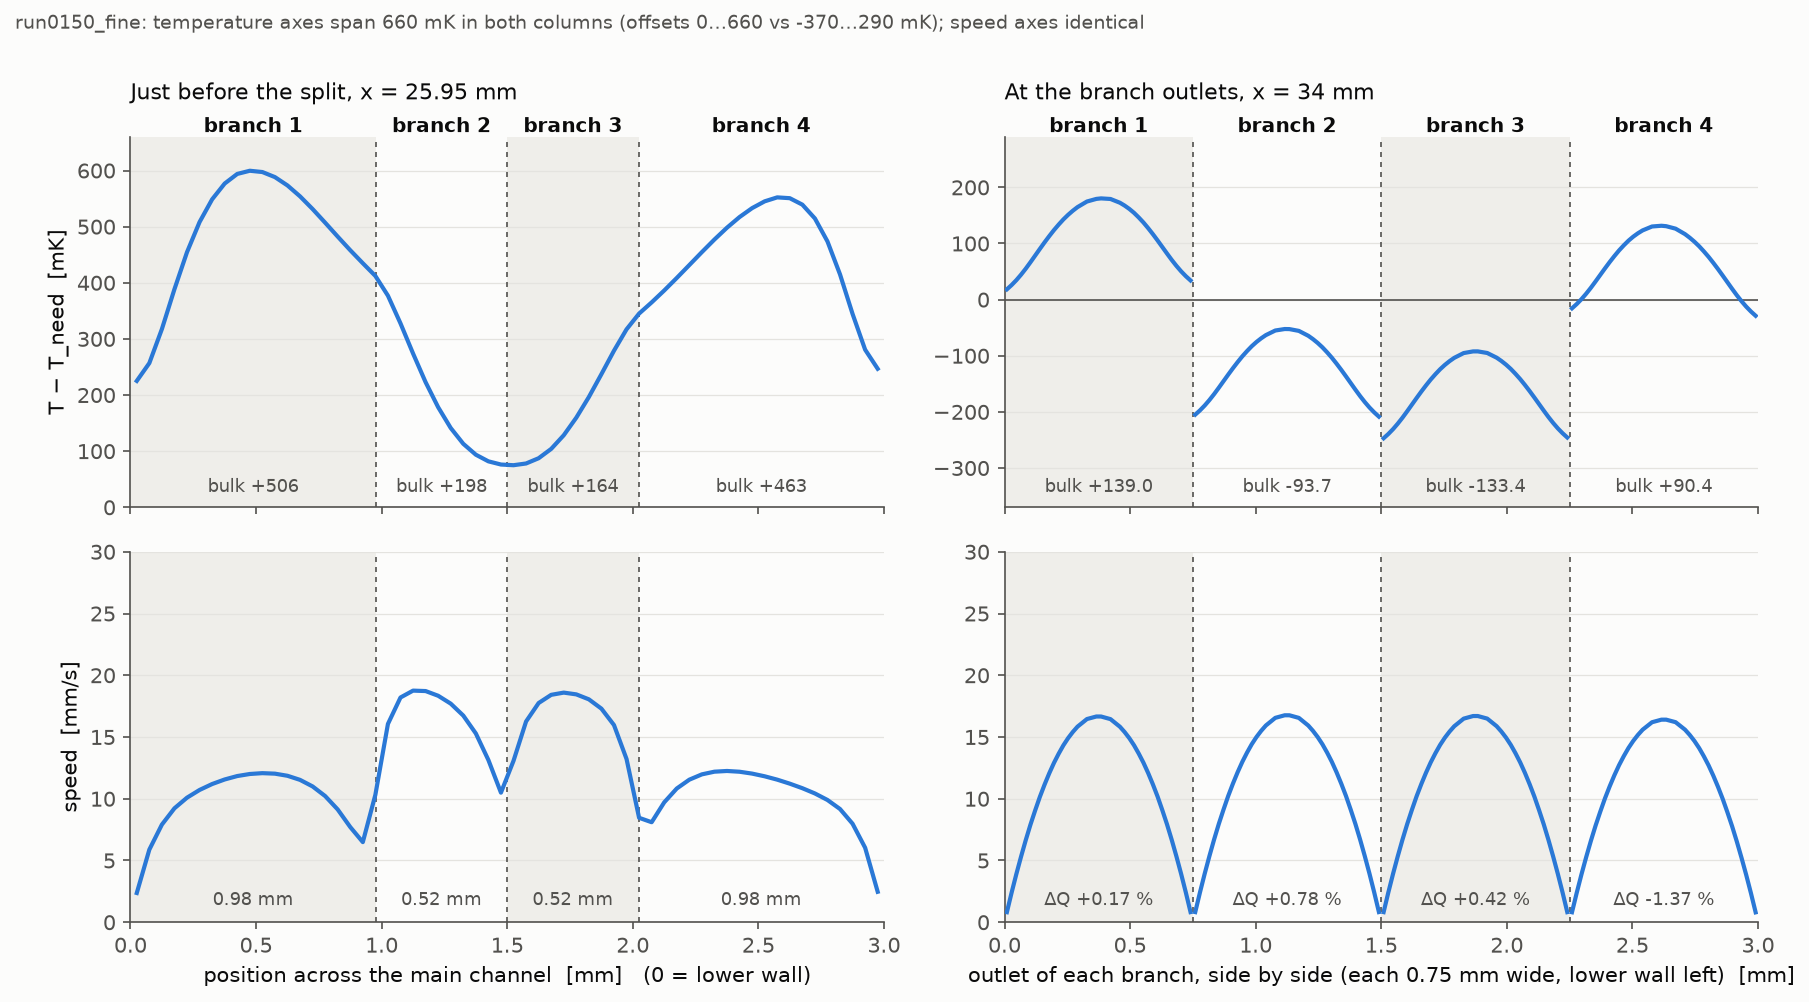
\includegraphics[width=0.95\textwidth,height=0.8\textheight,keepaspectratio]{runs/final_b2d_sine_presplit.png}
\caption{Cross-section just before the split, cut into the four branch inlets, next to each branch outlet.}
\end{figure}
\begin{figure}[H]\centering
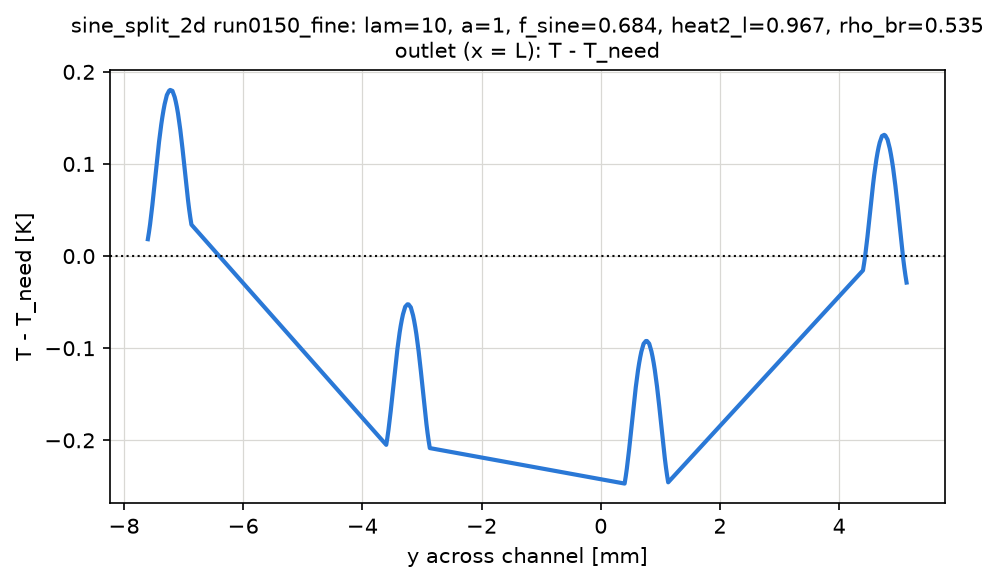
\includegraphics[width=0.75\textwidth,height=0.8\textheight,keepaspectratio]{runs/final_b2d_sine_outlet.png}
\caption{Outlet temperature (and, in 3D, the outlet plane).}
\end{figure}
\begin{figure}[H]\centering
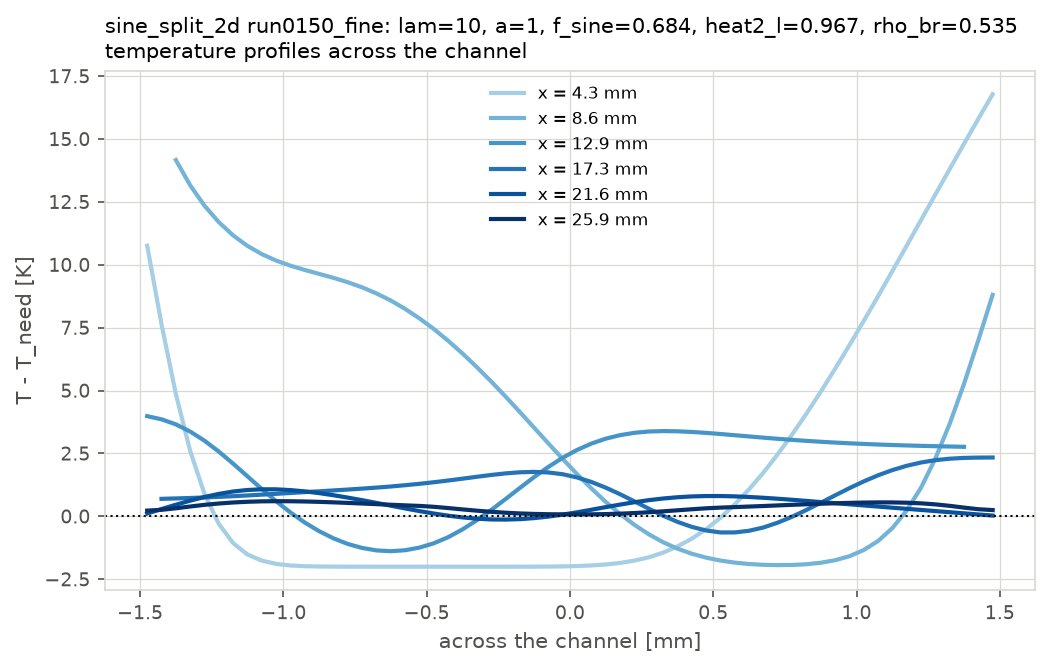
\includegraphics[width=0.62\textwidth,height=0.8\textheight,keepaspectratio]{runs/final_b2d_sine_slices.png}
\caption{Temperature profiles across the channel at several $x$ stations.}
\end{figure}
\begin{figure}[H]\centering
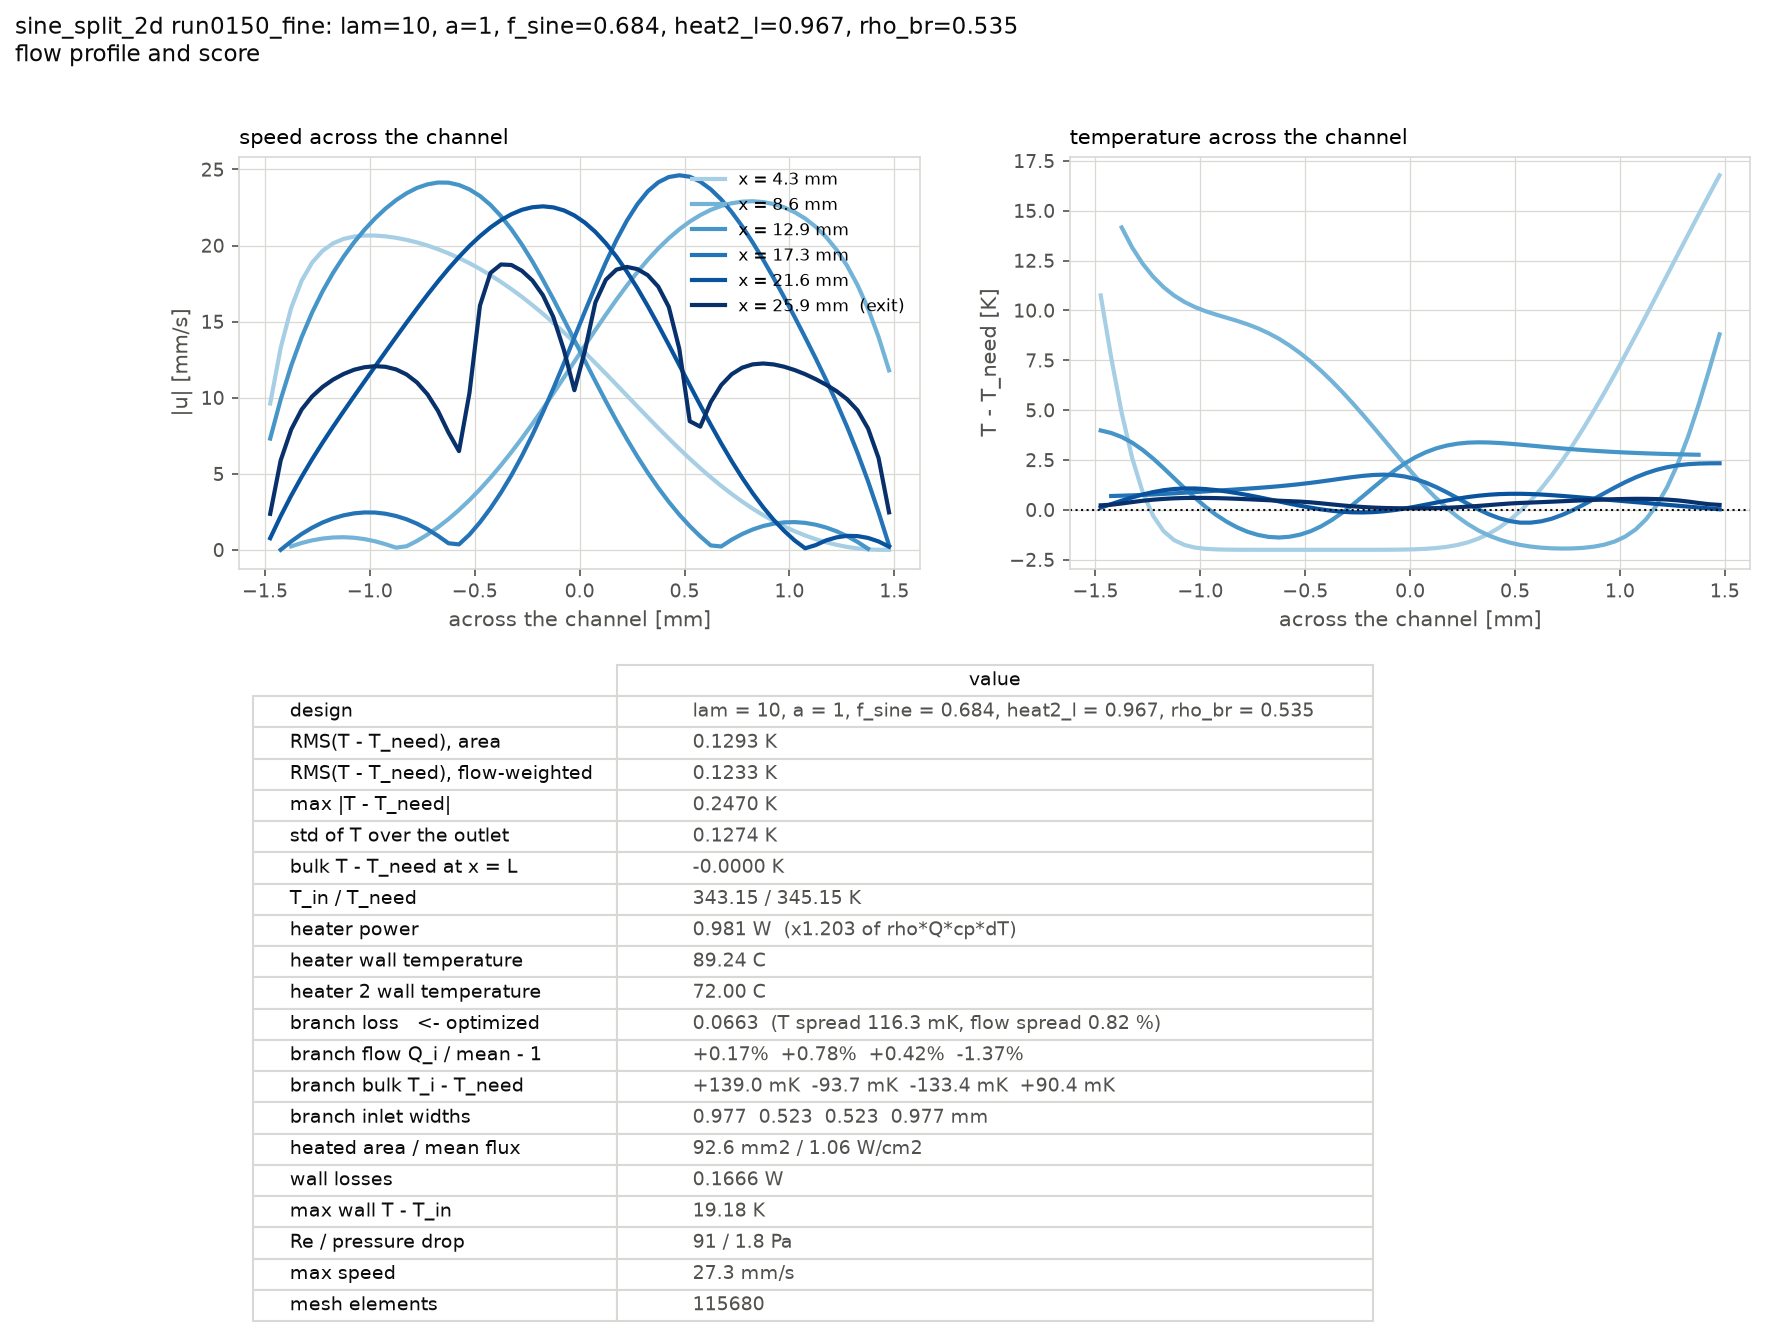
\includegraphics[width=0.8\textwidth,height=0.8\textheight,keepaspectratio]{runs/final_b2d_sine_profile.png}
\caption{Speed and temperature across the channel at several $x$ stations, and the full score table of the design.}
\end{figure}
\begin{figure}[H]\centering
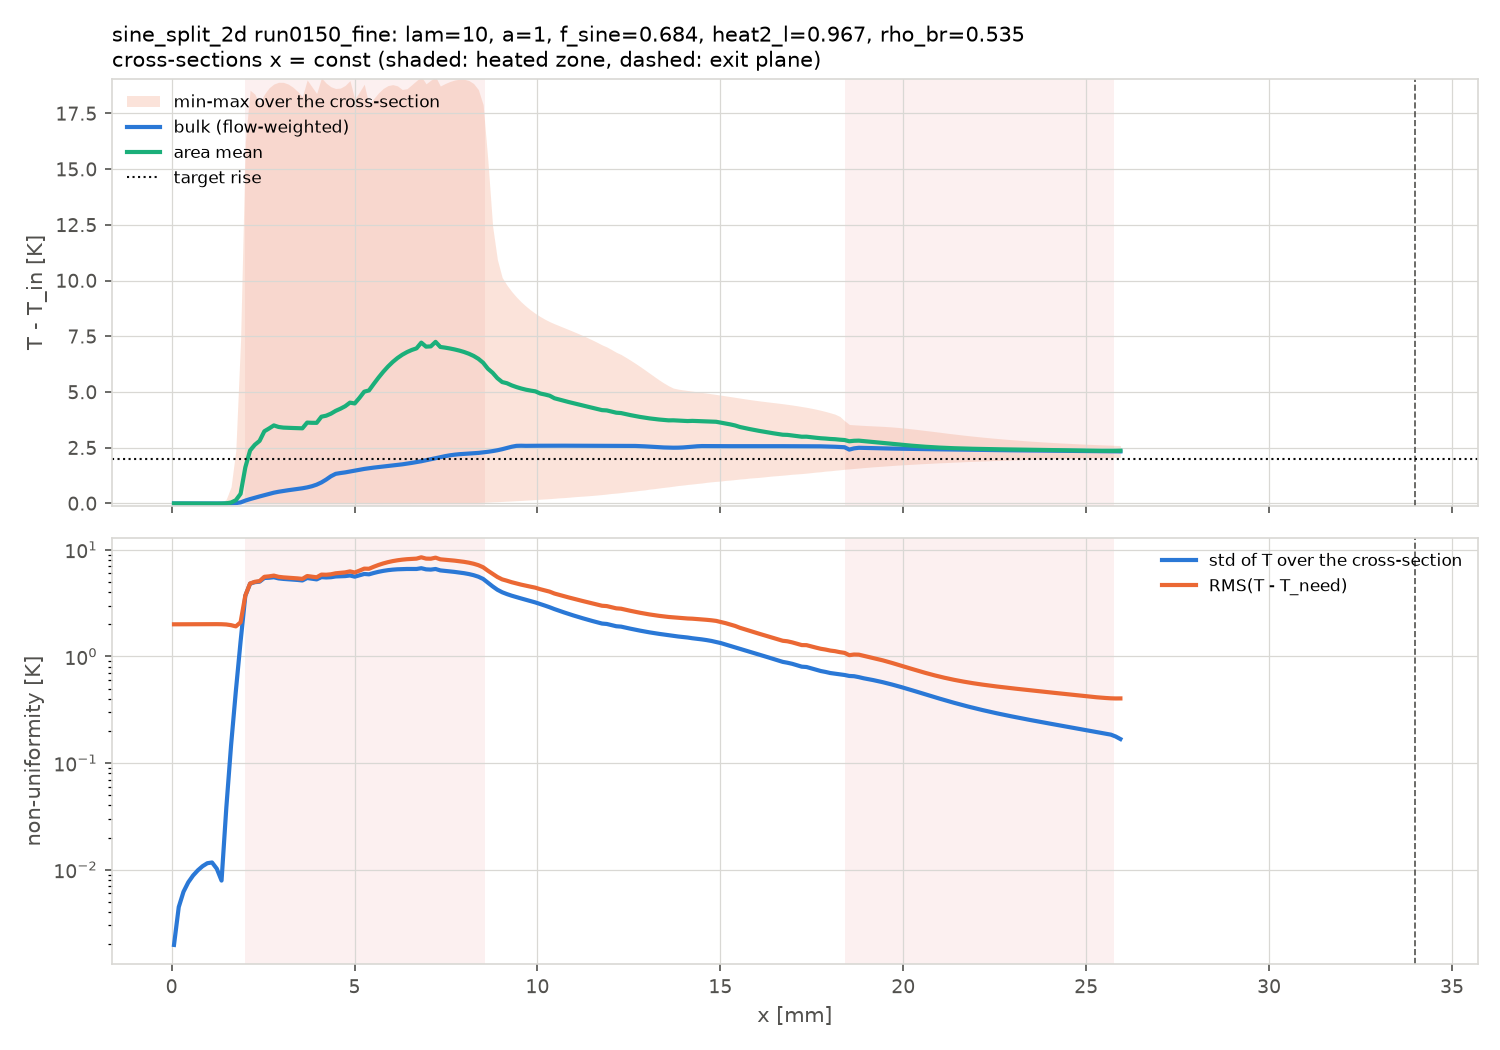
\includegraphics[width=0.8\textwidth,height=0.8\textheight,keepaspectratio]{runs/final_b2d_sine_along_x.png}
\caption{Bulk, mean, min and max temperature along the channel.}
\end{figure}
\begin{figure}[H]\centering
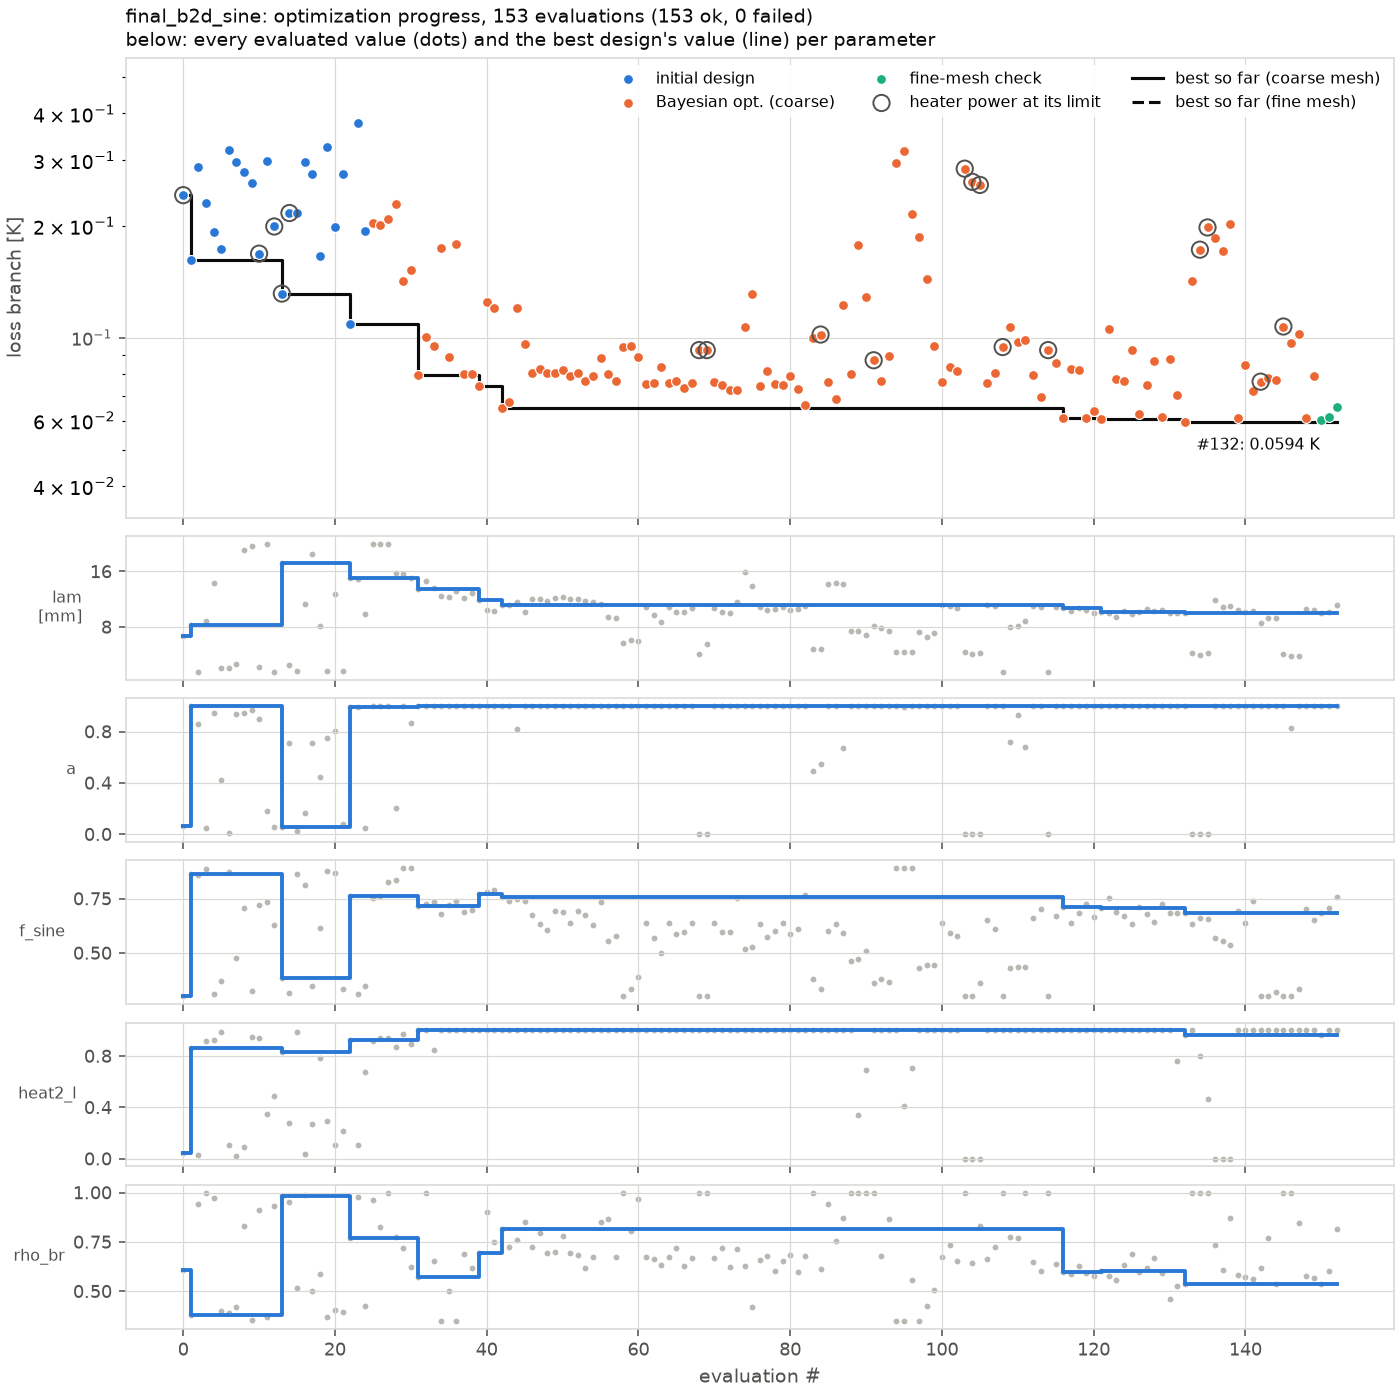
\includegraphics[width=0.85\textwidth]{runs/final_b2d_sine_progress_loss.png}
\caption{Search history: loss of every evaluation, best so far, and the parameters.}
\end{figure}
\clearpage
\subsubsection*{Branched serpentine + straight, BO best \#150: 12.3\mK, 3.9\,\%}
\noindent\texttt{runs/final\_b2d\_serp}\par\medskip
\begin{figure}[H]\centering
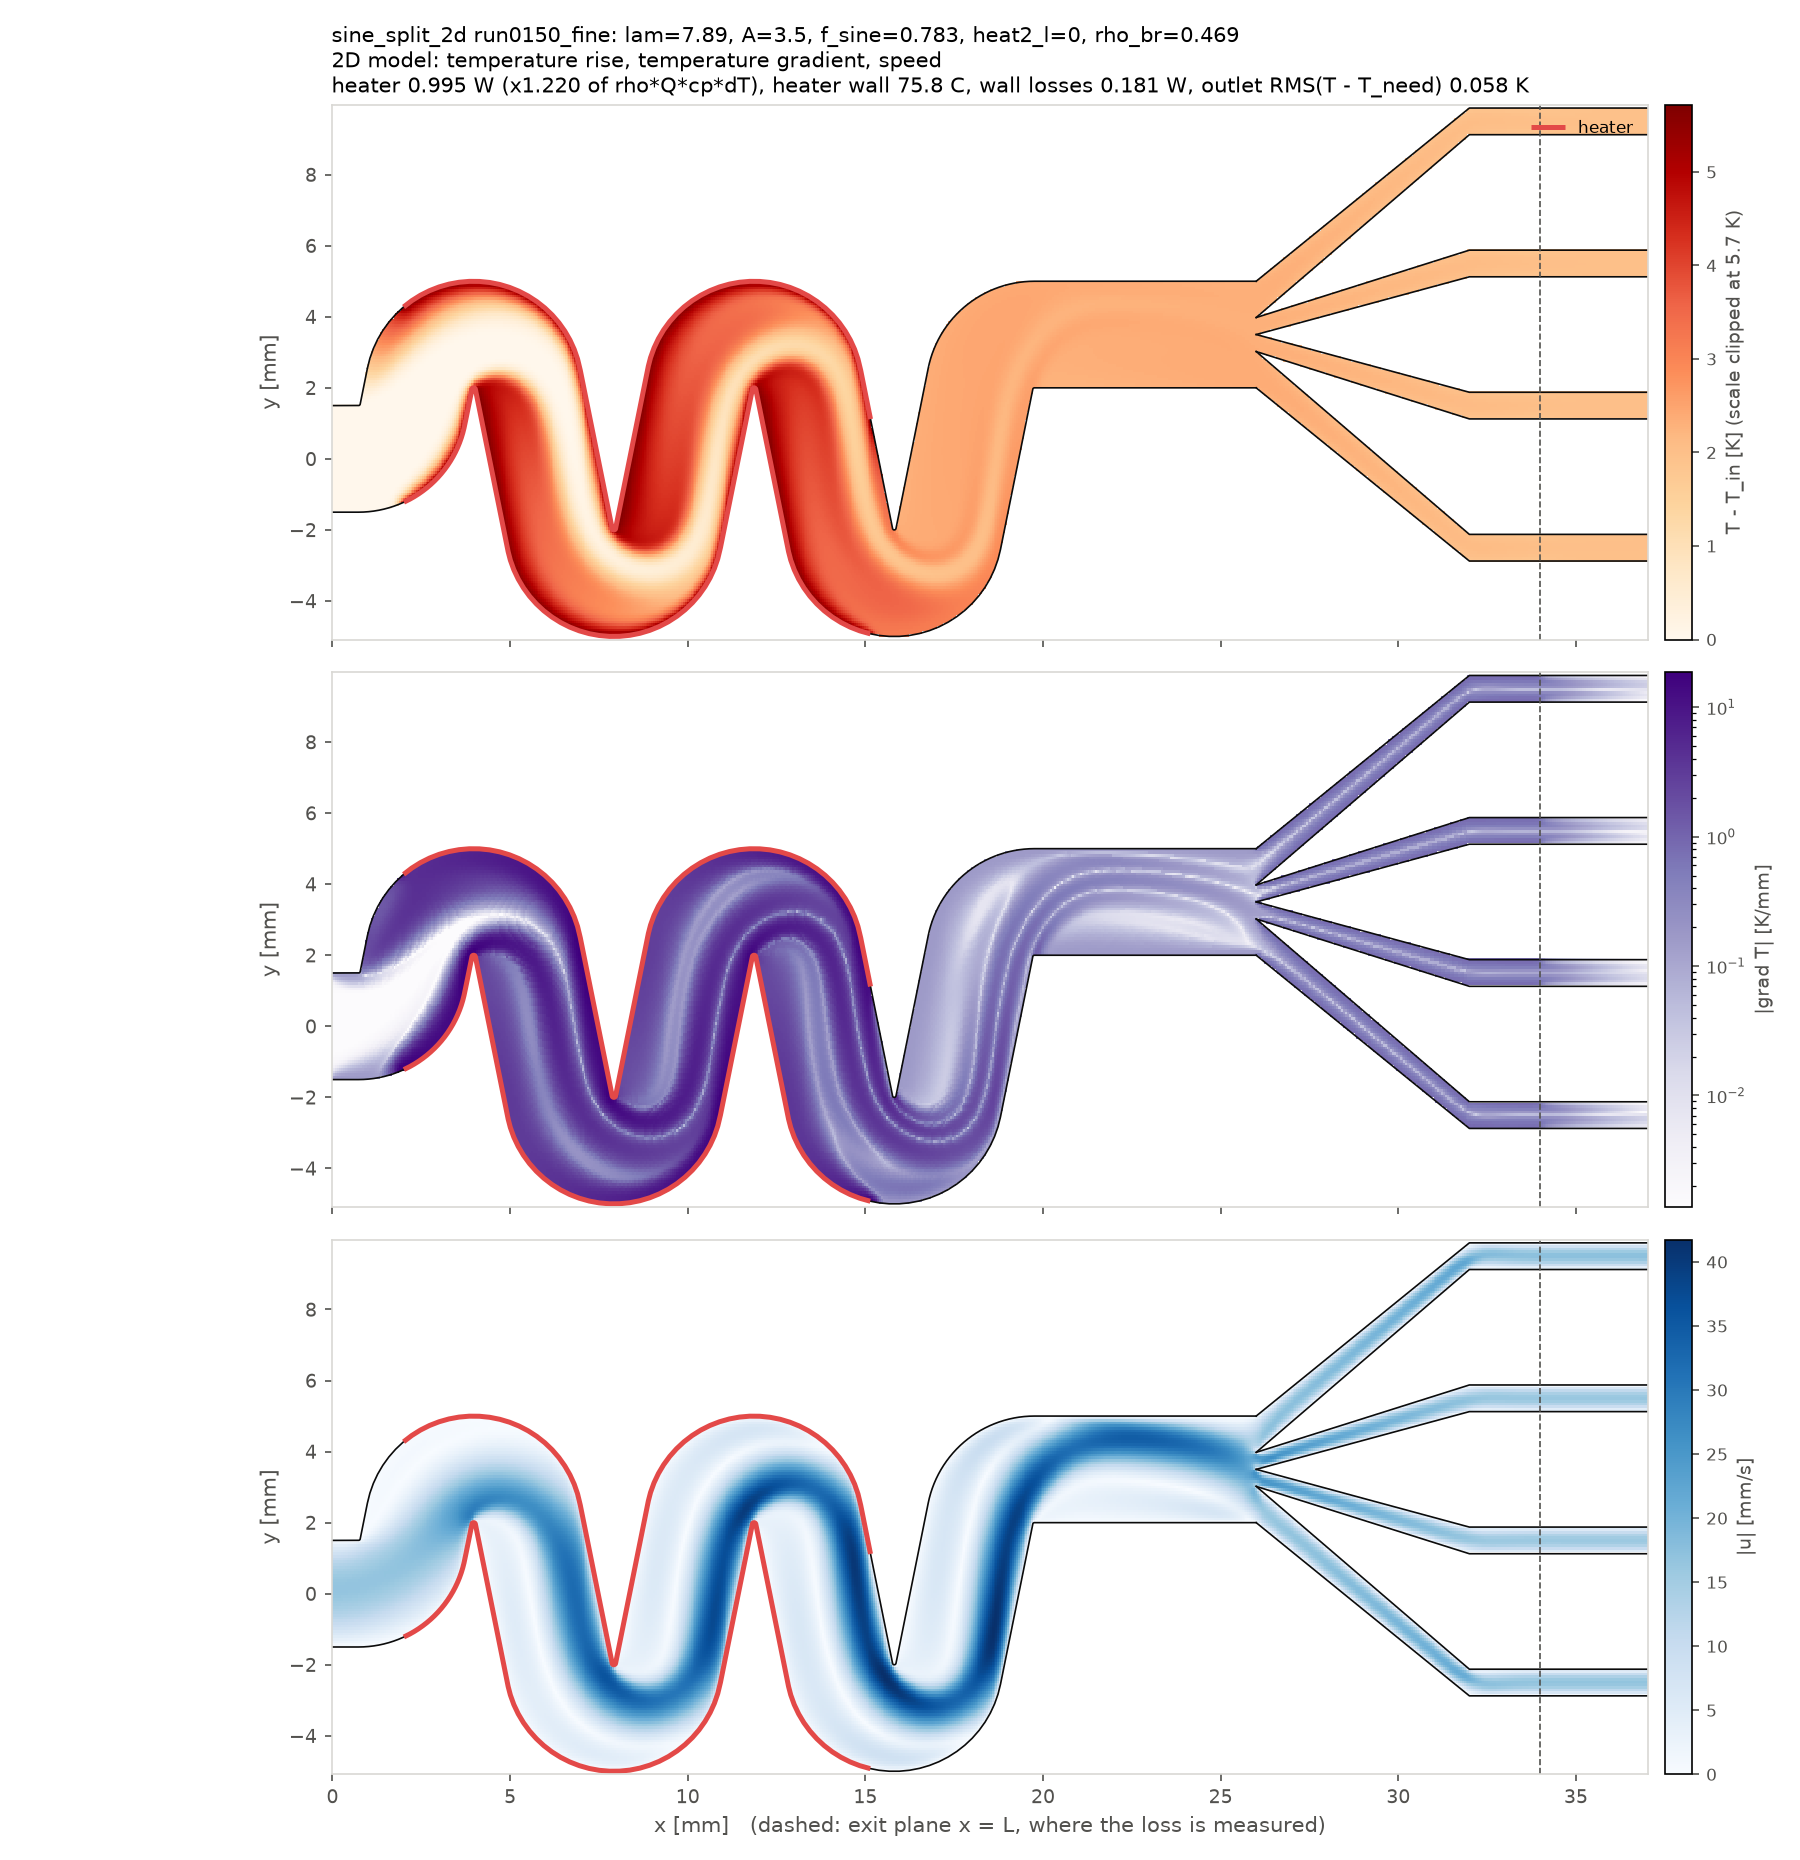
\includegraphics[width=0.95\textwidth,height=0.8\textheight,keepaspectratio]{runs/final_b2d_serp_maps.png}
\caption{Temperature rise, temperature gradient and speed (mid-depth plane in 3D). Red: heated wall. The title's ``outlet RMS'' is the area-weighted $\ell_{2,\mathrm{area}}$.}
\end{figure}
\begin{figure}[H]\centering
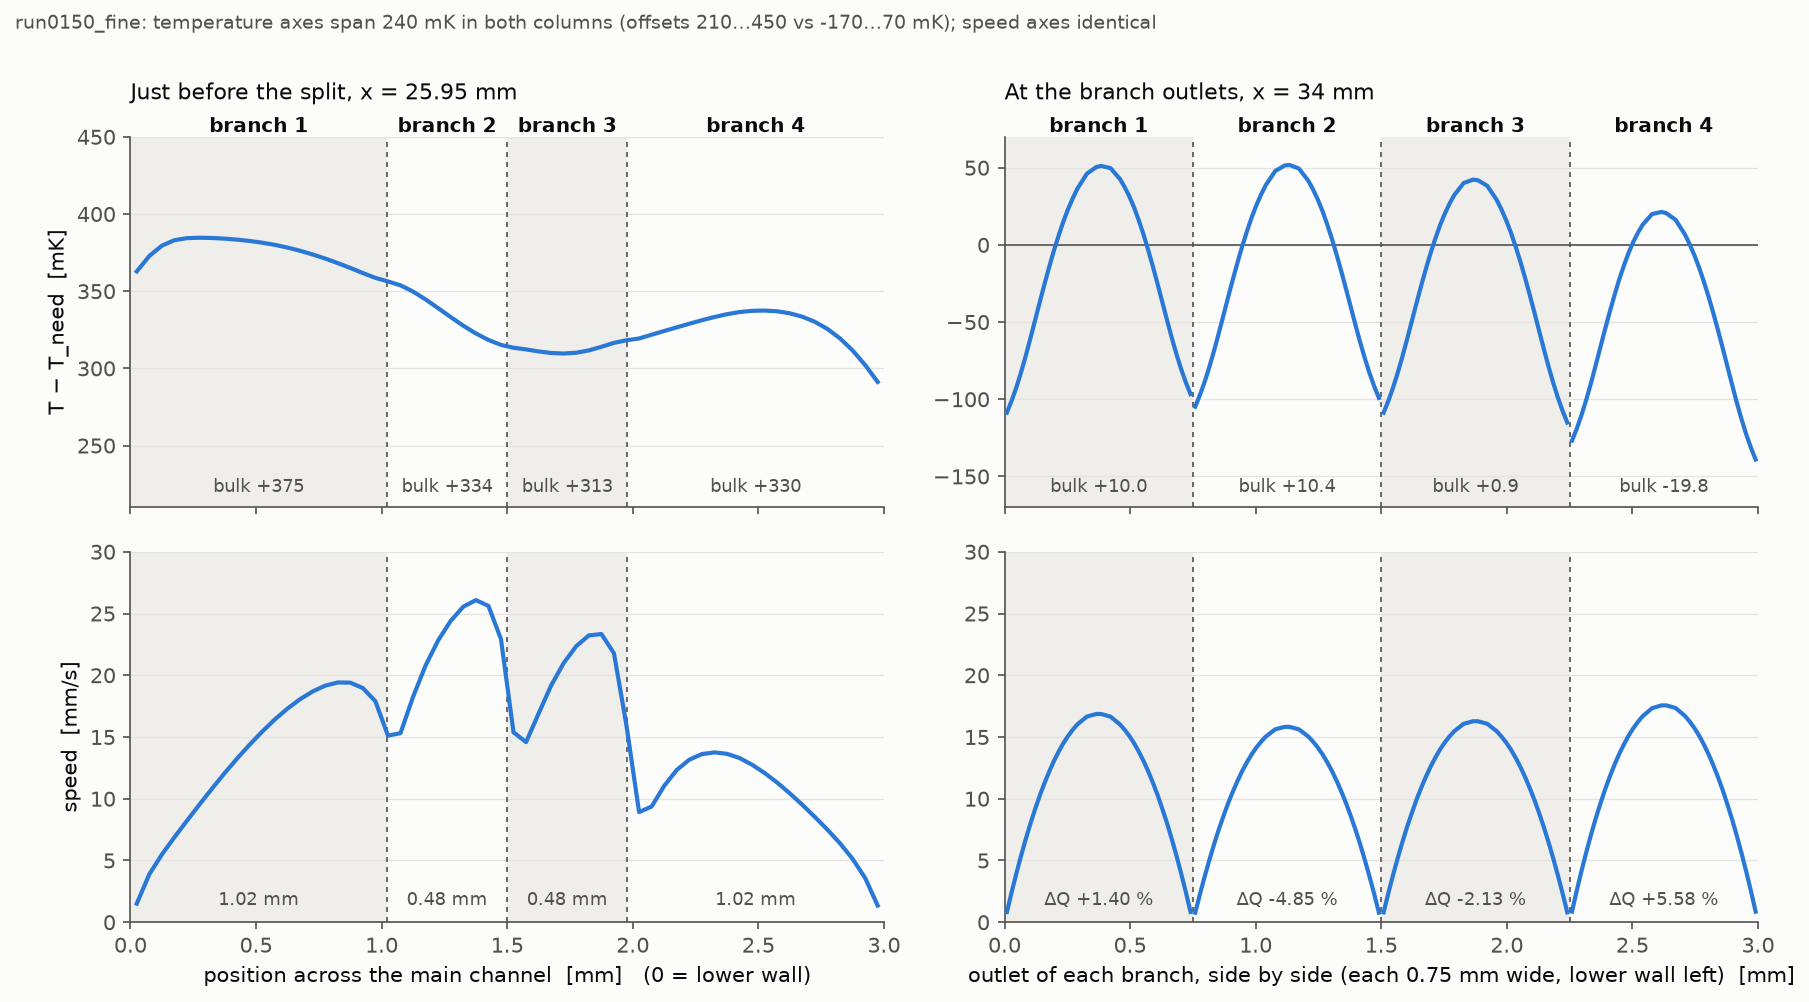
\includegraphics[width=0.95\textwidth,height=0.8\textheight,keepaspectratio]{runs/final_b2d_serp_presplit.png}
\caption{Cross-section just before the split, cut into the four branch inlets, next to each branch outlet.}
\end{figure}
\begin{figure}[H]\centering
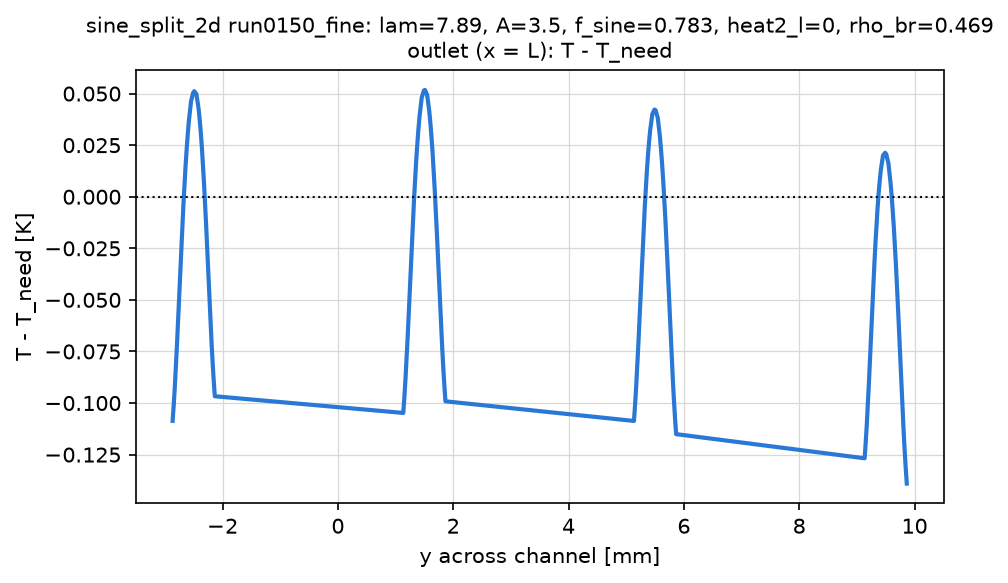
\includegraphics[width=0.75\textwidth,height=0.8\textheight,keepaspectratio]{runs/final_b2d_serp_outlet.png}
\caption{Outlet temperature (and, in 3D, the outlet plane).}
\end{figure}
\begin{figure}[H]\centering
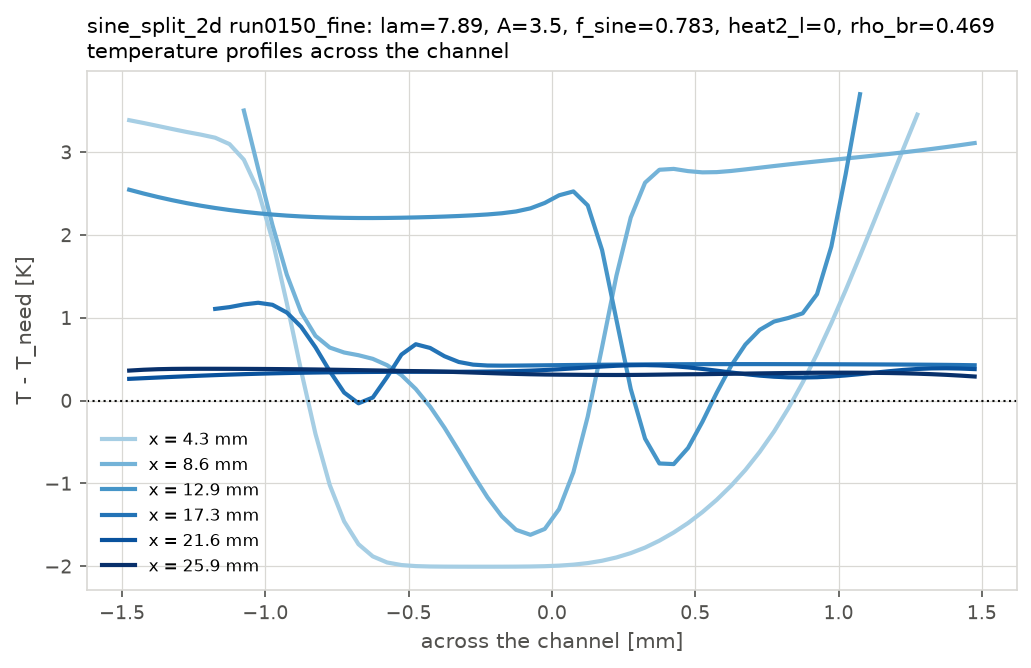
\includegraphics[width=0.62\textwidth,height=0.8\textheight,keepaspectratio]{runs/final_b2d_serp_slices.png}
\caption{Temperature profiles across the channel at several $x$ stations.}
\end{figure}
\begin{figure}[H]\centering
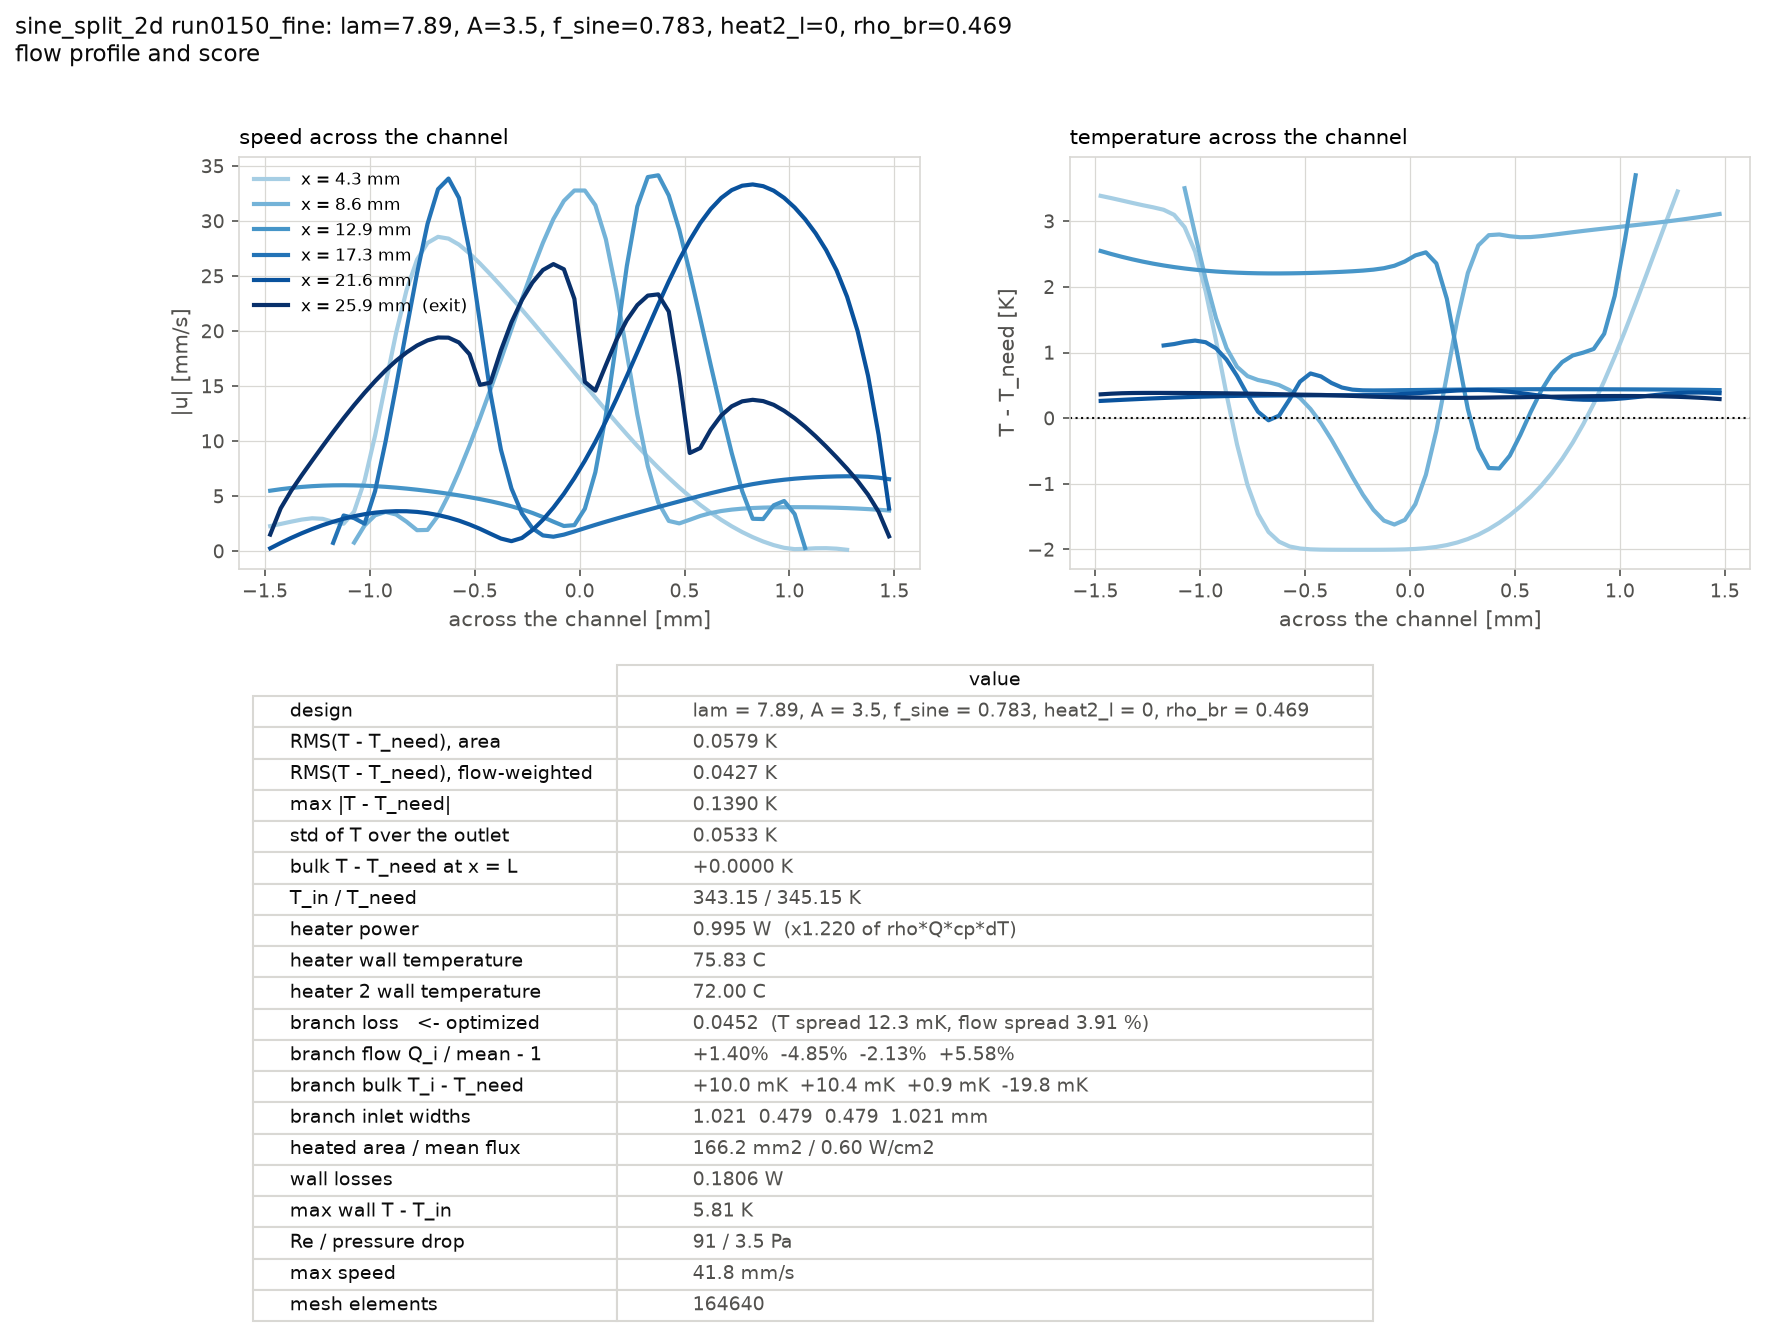
\includegraphics[width=0.8\textwidth,height=0.8\textheight,keepaspectratio]{runs/final_b2d_serp_profile.png}
\caption{Speed and temperature across the channel at several $x$ stations, and the full score table of the design.}
\end{figure}
\begin{figure}[H]\centering
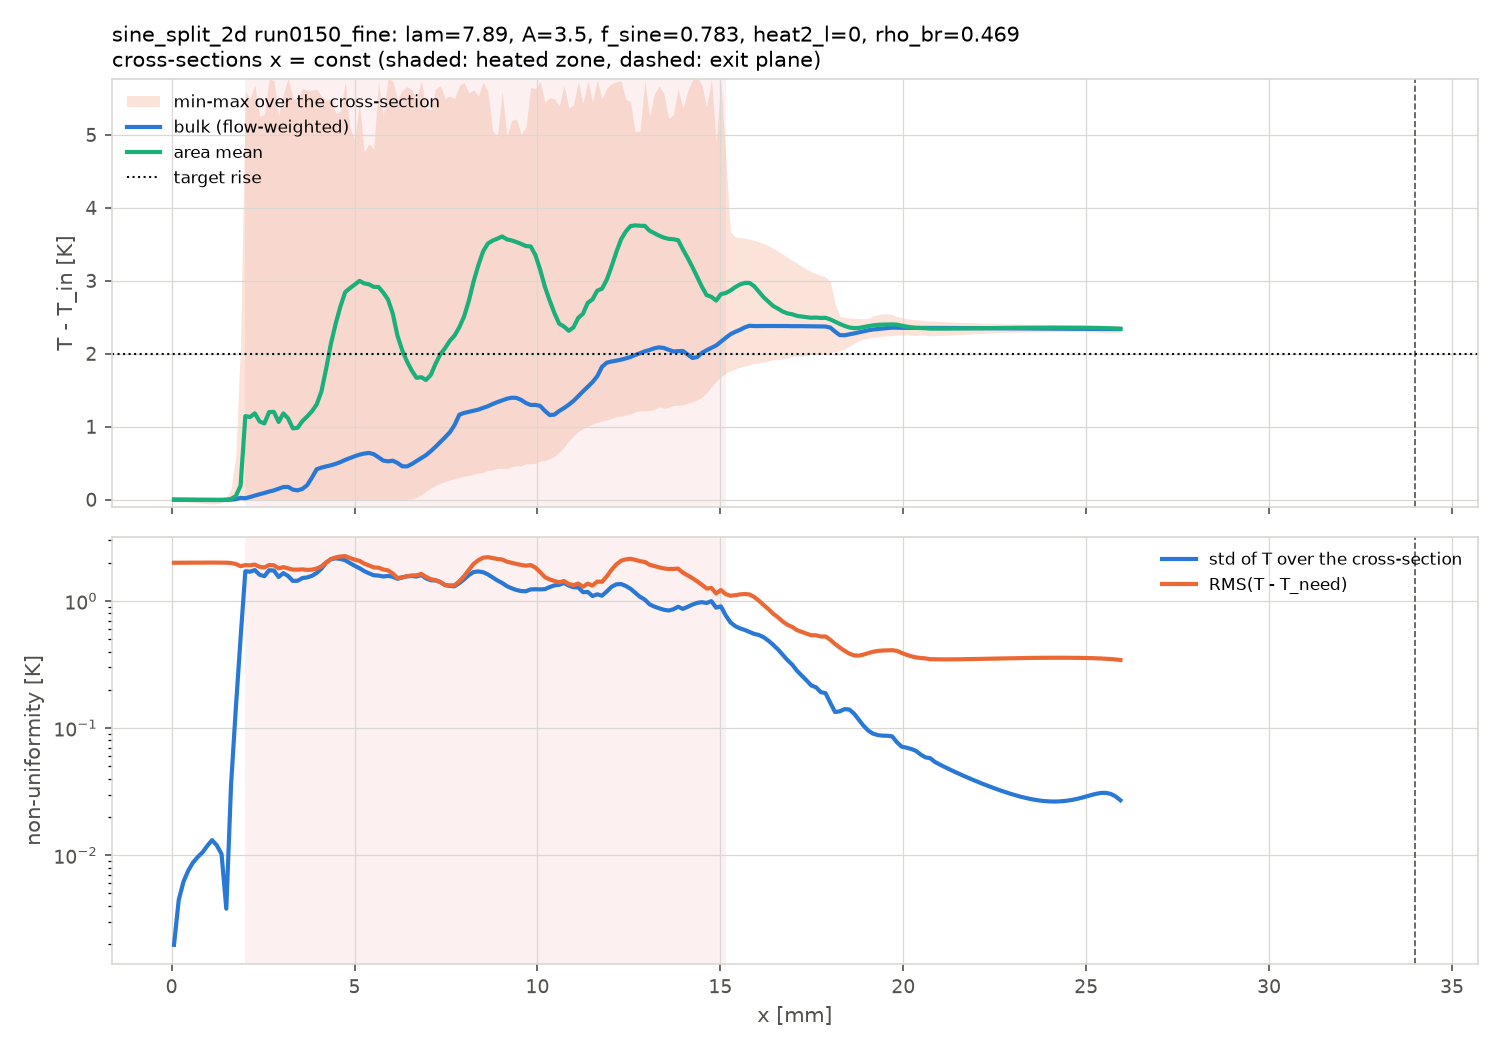
\includegraphics[width=0.8\textwidth,height=0.8\textheight,keepaspectratio]{runs/final_b2d_serp_along_x.png}
\caption{Bulk, mean, min and max temperature along the channel.}
\end{figure}
\begin{figure}[H]\centering
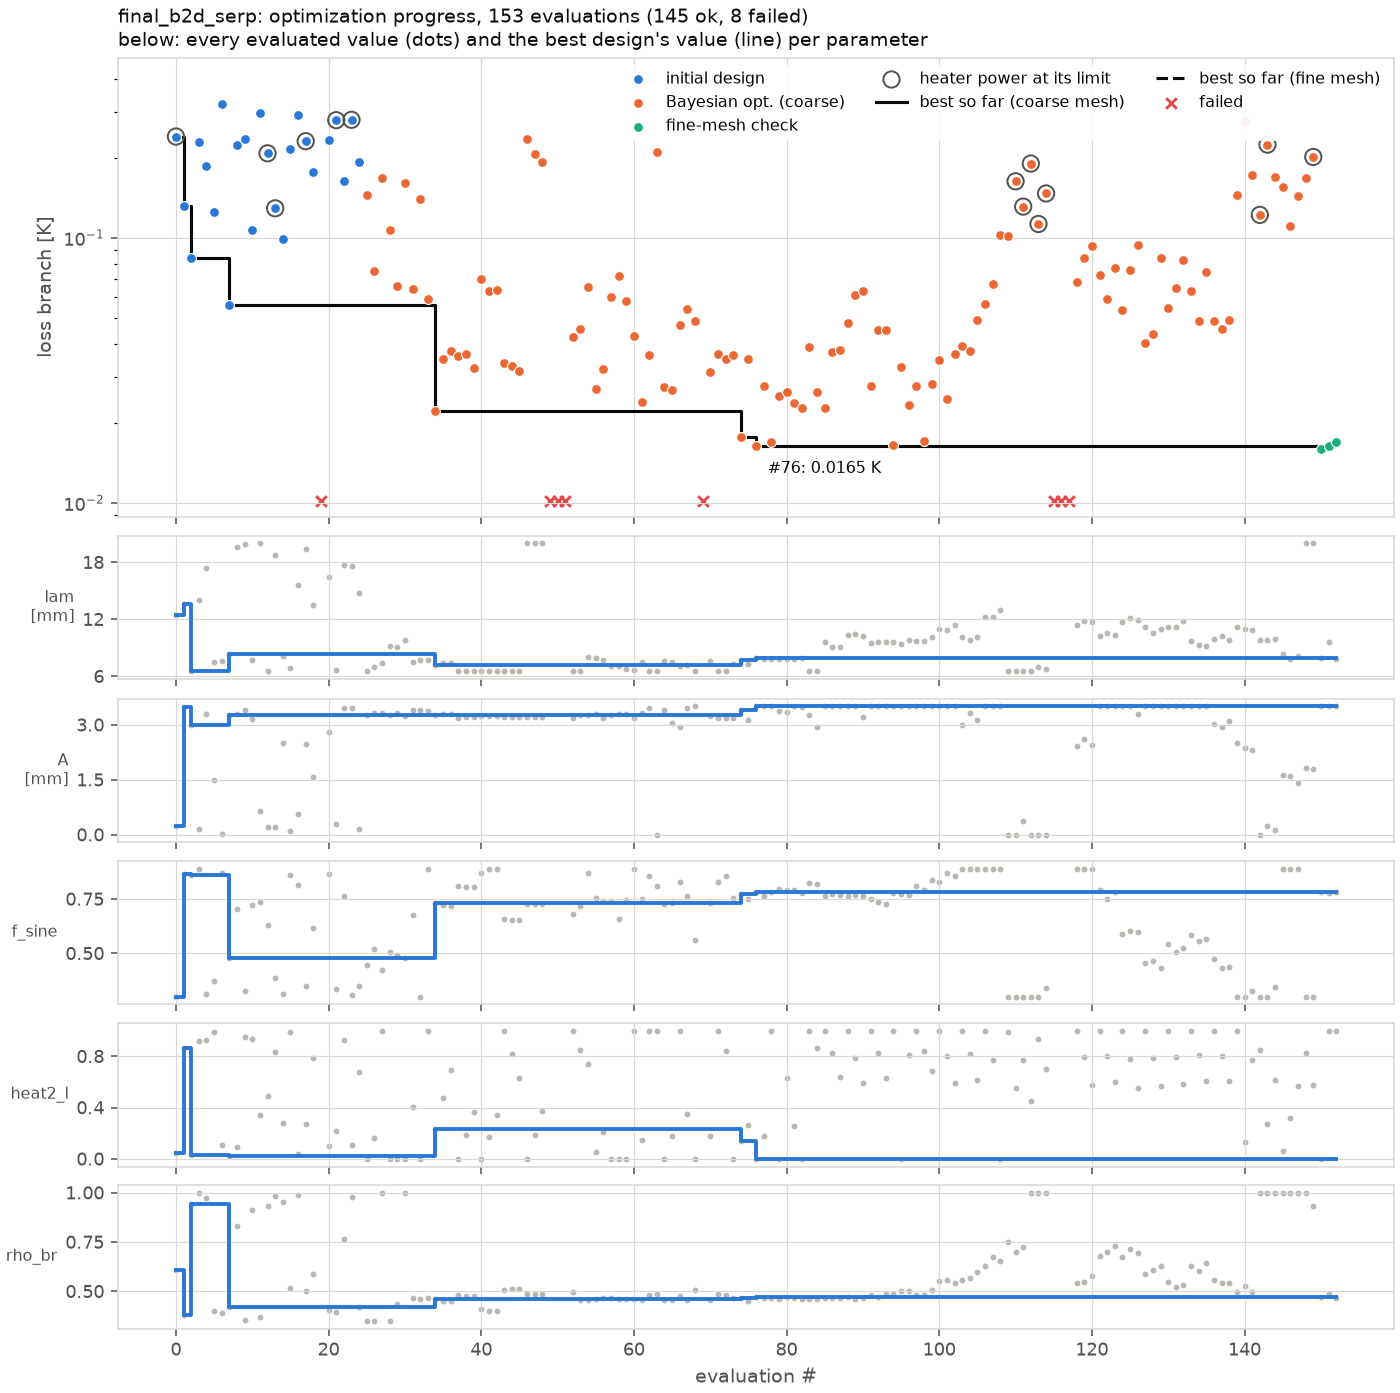
\includegraphics[width=0.85\textwidth]{runs/final_b2d_serp_progress_loss.png}
\caption{Search history: loss of every evaluation, best so far, and the parameters.}
\end{figure}
